
% Default to the notebook output style

    


% Inherit from the specified cell style.




    
\documentclass[11pt]{article}

    
    
    \usepackage[T1]{fontenc}
    % Nicer default font (+ math font) than Computer Modern for most use cases
    \usepackage{mathpazo}

    % Basic figure setup, for now with no caption control since it's done
    % automatically by Pandoc (which extracts ![](path) syntax from Markdown).
    \usepackage{graphicx}
    % We will generate all images so they have a width \maxwidth. This means
    % that they will get their normal width if they fit onto the page, but
    % are scaled down if they would overflow the margins.
    \makeatletter
    \def\maxwidth{\ifdim\Gin@nat@width>\linewidth\linewidth
    \else\Gin@nat@width\fi}
    \makeatother
    \let\Oldincludegraphics\includegraphics
    % Set max figure width to be 80% of text width, for now hardcoded.
    \renewcommand{\includegraphics}[1]{\Oldincludegraphics[width=.8\maxwidth]{#1}}
    % Ensure that by default, figures have no caption (until we provide a
    % proper Figure object with a Caption API and a way to capture that
    % in the conversion process - todo).
    \usepackage{caption}
    \DeclareCaptionLabelFormat{nolabel}{}
    \captionsetup{labelformat=nolabel}

    \usepackage{adjustbox} % Used to constrain images to a maximum size 
    \usepackage{xcolor} % Allow colors to be defined
    \usepackage{enumerate} % Needed for markdown enumerations to work
    \usepackage{geometry} % Used to adjust the document margins
    \usepackage{amsmath} % Equations
    \usepackage{amssymb} % Equations
    \usepackage{textcomp} % defines textquotesingle
    % Hack from http://tex.stackexchange.com/a/47451/13684:
    \AtBeginDocument{%
        \def\PYZsq{\textquotesingle}% Upright quotes in Pygmentized code
    }
    \usepackage{upquote} % Upright quotes for verbatim code
    \usepackage{eurosym} % defines \euro
    \usepackage[mathletters]{ucs} % Extended unicode (utf-8) support
    \usepackage[utf8x]{inputenc} % Allow utf-8 characters in the tex document
    \usepackage{fancyvrb} % verbatim replacement that allows latex
    \usepackage{grffile} % extends the file name processing of package graphics 
                         % to support a larger range 
    % The hyperref package gives us a pdf with properly built
    % internal navigation ('pdf bookmarks' for the table of contents,
    % internal cross-reference links, web links for URLs, etc.)
    \usepackage{hyperref}
    \usepackage{longtable} % longtable support required by pandoc >1.10
    \usepackage{booktabs}  % table support for pandoc > 1.12.2
    \usepackage[inline]{enumitem} % IRkernel/repr support (it uses the enumerate* environment)
    \usepackage[normalem]{ulem} % ulem is needed to support strikethroughs (\sout)
                                % normalem makes italics be italics, not underlines
    

    
    
    % Colors for the hyperref package
    \definecolor{urlcolor}{rgb}{0,.145,.698}
    \definecolor{linkcolor}{rgb}{.71,0.21,0.01}
    \definecolor{citecolor}{rgb}{.12,.54,.11}

    % ANSI colors
    \definecolor{ansi-black}{HTML}{3E424D}
    \definecolor{ansi-black-intense}{HTML}{282C36}
    \definecolor{ansi-red}{HTML}{E75C58}
    \definecolor{ansi-red-intense}{HTML}{B22B31}
    \definecolor{ansi-green}{HTML}{00A250}
    \definecolor{ansi-green-intense}{HTML}{007427}
    \definecolor{ansi-yellow}{HTML}{DDB62B}
    \definecolor{ansi-yellow-intense}{HTML}{B27D12}
    \definecolor{ansi-blue}{HTML}{208FFB}
    \definecolor{ansi-blue-intense}{HTML}{0065CA}
    \definecolor{ansi-magenta}{HTML}{D160C4}
    \definecolor{ansi-magenta-intense}{HTML}{A03196}
    \definecolor{ansi-cyan}{HTML}{60C6C8}
    \definecolor{ansi-cyan-intense}{HTML}{258F8F}
    \definecolor{ansi-white}{HTML}{C5C1B4}
    \definecolor{ansi-white-intense}{HTML}{A1A6B2}

    % commands and environments needed by pandoc snippets
    % extracted from the output of `pandoc -s`
    \providecommand{\tightlist}{%
      \setlength{\itemsep}{0pt}\setlength{\parskip}{0pt}}
    \DefineVerbatimEnvironment{Highlighting}{Verbatim}{commandchars=\\\{\}}
    % Add ',fontsize=\small' for more characters per line
    \newenvironment{Shaded}{}{}
    \newcommand{\KeywordTok}[1]{\textcolor[rgb]{0.00,0.44,0.13}{\textbf{{#1}}}}
    \newcommand{\DataTypeTok}[1]{\textcolor[rgb]{0.56,0.13,0.00}{{#1}}}
    \newcommand{\DecValTok}[1]{\textcolor[rgb]{0.25,0.63,0.44}{{#1}}}
    \newcommand{\BaseNTok}[1]{\textcolor[rgb]{0.25,0.63,0.44}{{#1}}}
    \newcommand{\FloatTok}[1]{\textcolor[rgb]{0.25,0.63,0.44}{{#1}}}
    \newcommand{\CharTok}[1]{\textcolor[rgb]{0.25,0.44,0.63}{{#1}}}
    \newcommand{\StringTok}[1]{\textcolor[rgb]{0.25,0.44,0.63}{{#1}}}
    \newcommand{\CommentTok}[1]{\textcolor[rgb]{0.38,0.63,0.69}{\textit{{#1}}}}
    \newcommand{\OtherTok}[1]{\textcolor[rgb]{0.00,0.44,0.13}{{#1}}}
    \newcommand{\AlertTok}[1]{\textcolor[rgb]{1.00,0.00,0.00}{\textbf{{#1}}}}
    \newcommand{\FunctionTok}[1]{\textcolor[rgb]{0.02,0.16,0.49}{{#1}}}
    \newcommand{\RegionMarkerTok}[1]{{#1}}
    \newcommand{\ErrorTok}[1]{\textcolor[rgb]{1.00,0.00,0.00}{\textbf{{#1}}}}
    \newcommand{\NormalTok}[1]{{#1}}
    
    % Additional commands for more recent versions of Pandoc
    \newcommand{\ConstantTok}[1]{\textcolor[rgb]{0.53,0.00,0.00}{{#1}}}
    \newcommand{\SpecialCharTok}[1]{\textcolor[rgb]{0.25,0.44,0.63}{{#1}}}
    \newcommand{\VerbatimStringTok}[1]{\textcolor[rgb]{0.25,0.44,0.63}{{#1}}}
    \newcommand{\SpecialStringTok}[1]{\textcolor[rgb]{0.73,0.40,0.53}{{#1}}}
    \newcommand{\ImportTok}[1]{{#1}}
    \newcommand{\DocumentationTok}[1]{\textcolor[rgb]{0.73,0.13,0.13}{\textit{{#1}}}}
    \newcommand{\AnnotationTok}[1]{\textcolor[rgb]{0.38,0.63,0.69}{\textbf{\textit{{#1}}}}}
    \newcommand{\CommentVarTok}[1]{\textcolor[rgb]{0.38,0.63,0.69}{\textbf{\textit{{#1}}}}}
    \newcommand{\VariableTok}[1]{\textcolor[rgb]{0.10,0.09,0.49}{{#1}}}
    \newcommand{\ControlFlowTok}[1]{\textcolor[rgb]{0.00,0.44,0.13}{\textbf{{#1}}}}
    \newcommand{\OperatorTok}[1]{\textcolor[rgb]{0.40,0.40,0.40}{{#1}}}
    \newcommand{\BuiltInTok}[1]{{#1}}
    \newcommand{\ExtensionTok}[1]{{#1}}
    \newcommand{\PreprocessorTok}[1]{\textcolor[rgb]{0.74,0.48,0.00}{{#1}}}
    \newcommand{\AttributeTok}[1]{\textcolor[rgb]{0.49,0.56,0.16}{{#1}}}
    \newcommand{\InformationTok}[1]{\textcolor[rgb]{0.38,0.63,0.69}{\textbf{\textit{{#1}}}}}
    \newcommand{\WarningTok}[1]{\textcolor[rgb]{0.38,0.63,0.69}{\textbf{\textit{{#1}}}}}
    
    
    % Define a nice break command that doesn't care if a line doesn't already
    % exist.
    \def\br{\hspace*{\fill} \\* }
    % Math Jax compatability definitions
    \def\gt{>}
    \def\lt{<}
    % Document parameters
    \title{DIP\_HW10}
    
    
    

    % Pygments definitions
    
\makeatletter
\def\PY@reset{\let\PY@it=\relax \let\PY@bf=\relax%
    \let\PY@ul=\relax \let\PY@tc=\relax%
    \let\PY@bc=\relax \let\PY@ff=\relax}
\def\PY@tok#1{\csname PY@tok@#1\endcsname}
\def\PY@toks#1+{\ifx\relax#1\empty\else%
    \PY@tok{#1}\expandafter\PY@toks\fi}
\def\PY@do#1{\PY@bc{\PY@tc{\PY@ul{%
    \PY@it{\PY@bf{\PY@ff{#1}}}}}}}
\def\PY#1#2{\PY@reset\PY@toks#1+\relax+\PY@do{#2}}

\expandafter\def\csname PY@tok@w\endcsname{\def\PY@tc##1{\textcolor[rgb]{0.73,0.73,0.73}{##1}}}
\expandafter\def\csname PY@tok@c\endcsname{\let\PY@it=\textit\def\PY@tc##1{\textcolor[rgb]{0.25,0.50,0.50}{##1}}}
\expandafter\def\csname PY@tok@cp\endcsname{\def\PY@tc##1{\textcolor[rgb]{0.74,0.48,0.00}{##1}}}
\expandafter\def\csname PY@tok@k\endcsname{\let\PY@bf=\textbf\def\PY@tc##1{\textcolor[rgb]{0.00,0.50,0.00}{##1}}}
\expandafter\def\csname PY@tok@kp\endcsname{\def\PY@tc##1{\textcolor[rgb]{0.00,0.50,0.00}{##1}}}
\expandafter\def\csname PY@tok@kt\endcsname{\def\PY@tc##1{\textcolor[rgb]{0.69,0.00,0.25}{##1}}}
\expandafter\def\csname PY@tok@o\endcsname{\def\PY@tc##1{\textcolor[rgb]{0.40,0.40,0.40}{##1}}}
\expandafter\def\csname PY@tok@ow\endcsname{\let\PY@bf=\textbf\def\PY@tc##1{\textcolor[rgb]{0.67,0.13,1.00}{##1}}}
\expandafter\def\csname PY@tok@nb\endcsname{\def\PY@tc##1{\textcolor[rgb]{0.00,0.50,0.00}{##1}}}
\expandafter\def\csname PY@tok@nf\endcsname{\def\PY@tc##1{\textcolor[rgb]{0.00,0.00,1.00}{##1}}}
\expandafter\def\csname PY@tok@nc\endcsname{\let\PY@bf=\textbf\def\PY@tc##1{\textcolor[rgb]{0.00,0.00,1.00}{##1}}}
\expandafter\def\csname PY@tok@nn\endcsname{\let\PY@bf=\textbf\def\PY@tc##1{\textcolor[rgb]{0.00,0.00,1.00}{##1}}}
\expandafter\def\csname PY@tok@ne\endcsname{\let\PY@bf=\textbf\def\PY@tc##1{\textcolor[rgb]{0.82,0.25,0.23}{##1}}}
\expandafter\def\csname PY@tok@nv\endcsname{\def\PY@tc##1{\textcolor[rgb]{0.10,0.09,0.49}{##1}}}
\expandafter\def\csname PY@tok@no\endcsname{\def\PY@tc##1{\textcolor[rgb]{0.53,0.00,0.00}{##1}}}
\expandafter\def\csname PY@tok@nl\endcsname{\def\PY@tc##1{\textcolor[rgb]{0.63,0.63,0.00}{##1}}}
\expandafter\def\csname PY@tok@ni\endcsname{\let\PY@bf=\textbf\def\PY@tc##1{\textcolor[rgb]{0.60,0.60,0.60}{##1}}}
\expandafter\def\csname PY@tok@na\endcsname{\def\PY@tc##1{\textcolor[rgb]{0.49,0.56,0.16}{##1}}}
\expandafter\def\csname PY@tok@nt\endcsname{\let\PY@bf=\textbf\def\PY@tc##1{\textcolor[rgb]{0.00,0.50,0.00}{##1}}}
\expandafter\def\csname PY@tok@nd\endcsname{\def\PY@tc##1{\textcolor[rgb]{0.67,0.13,1.00}{##1}}}
\expandafter\def\csname PY@tok@s\endcsname{\def\PY@tc##1{\textcolor[rgb]{0.73,0.13,0.13}{##1}}}
\expandafter\def\csname PY@tok@sd\endcsname{\let\PY@it=\textit\def\PY@tc##1{\textcolor[rgb]{0.73,0.13,0.13}{##1}}}
\expandafter\def\csname PY@tok@si\endcsname{\let\PY@bf=\textbf\def\PY@tc##1{\textcolor[rgb]{0.73,0.40,0.53}{##1}}}
\expandafter\def\csname PY@tok@se\endcsname{\let\PY@bf=\textbf\def\PY@tc##1{\textcolor[rgb]{0.73,0.40,0.13}{##1}}}
\expandafter\def\csname PY@tok@sr\endcsname{\def\PY@tc##1{\textcolor[rgb]{0.73,0.40,0.53}{##1}}}
\expandafter\def\csname PY@tok@ss\endcsname{\def\PY@tc##1{\textcolor[rgb]{0.10,0.09,0.49}{##1}}}
\expandafter\def\csname PY@tok@sx\endcsname{\def\PY@tc##1{\textcolor[rgb]{0.00,0.50,0.00}{##1}}}
\expandafter\def\csname PY@tok@m\endcsname{\def\PY@tc##1{\textcolor[rgb]{0.40,0.40,0.40}{##1}}}
\expandafter\def\csname PY@tok@gh\endcsname{\let\PY@bf=\textbf\def\PY@tc##1{\textcolor[rgb]{0.00,0.00,0.50}{##1}}}
\expandafter\def\csname PY@tok@gu\endcsname{\let\PY@bf=\textbf\def\PY@tc##1{\textcolor[rgb]{0.50,0.00,0.50}{##1}}}
\expandafter\def\csname PY@tok@gd\endcsname{\def\PY@tc##1{\textcolor[rgb]{0.63,0.00,0.00}{##1}}}
\expandafter\def\csname PY@tok@gi\endcsname{\def\PY@tc##1{\textcolor[rgb]{0.00,0.63,0.00}{##1}}}
\expandafter\def\csname PY@tok@gr\endcsname{\def\PY@tc##1{\textcolor[rgb]{1.00,0.00,0.00}{##1}}}
\expandafter\def\csname PY@tok@ge\endcsname{\let\PY@it=\textit}
\expandafter\def\csname PY@tok@gs\endcsname{\let\PY@bf=\textbf}
\expandafter\def\csname PY@tok@gp\endcsname{\let\PY@bf=\textbf\def\PY@tc##1{\textcolor[rgb]{0.00,0.00,0.50}{##1}}}
\expandafter\def\csname PY@tok@go\endcsname{\def\PY@tc##1{\textcolor[rgb]{0.53,0.53,0.53}{##1}}}
\expandafter\def\csname PY@tok@gt\endcsname{\def\PY@tc##1{\textcolor[rgb]{0.00,0.27,0.87}{##1}}}
\expandafter\def\csname PY@tok@err\endcsname{\def\PY@bc##1{\setlength{\fboxsep}{0pt}\fcolorbox[rgb]{1.00,0.00,0.00}{1,1,1}{\strut ##1}}}
\expandafter\def\csname PY@tok@kc\endcsname{\let\PY@bf=\textbf\def\PY@tc##1{\textcolor[rgb]{0.00,0.50,0.00}{##1}}}
\expandafter\def\csname PY@tok@kd\endcsname{\let\PY@bf=\textbf\def\PY@tc##1{\textcolor[rgb]{0.00,0.50,0.00}{##1}}}
\expandafter\def\csname PY@tok@kn\endcsname{\let\PY@bf=\textbf\def\PY@tc##1{\textcolor[rgb]{0.00,0.50,0.00}{##1}}}
\expandafter\def\csname PY@tok@kr\endcsname{\let\PY@bf=\textbf\def\PY@tc##1{\textcolor[rgb]{0.00,0.50,0.00}{##1}}}
\expandafter\def\csname PY@tok@bp\endcsname{\def\PY@tc##1{\textcolor[rgb]{0.00,0.50,0.00}{##1}}}
\expandafter\def\csname PY@tok@fm\endcsname{\def\PY@tc##1{\textcolor[rgb]{0.00,0.00,1.00}{##1}}}
\expandafter\def\csname PY@tok@vc\endcsname{\def\PY@tc##1{\textcolor[rgb]{0.10,0.09,0.49}{##1}}}
\expandafter\def\csname PY@tok@vg\endcsname{\def\PY@tc##1{\textcolor[rgb]{0.10,0.09,0.49}{##1}}}
\expandafter\def\csname PY@tok@vi\endcsname{\def\PY@tc##1{\textcolor[rgb]{0.10,0.09,0.49}{##1}}}
\expandafter\def\csname PY@tok@vm\endcsname{\def\PY@tc##1{\textcolor[rgb]{0.10,0.09,0.49}{##1}}}
\expandafter\def\csname PY@tok@sa\endcsname{\def\PY@tc##1{\textcolor[rgb]{0.73,0.13,0.13}{##1}}}
\expandafter\def\csname PY@tok@sb\endcsname{\def\PY@tc##1{\textcolor[rgb]{0.73,0.13,0.13}{##1}}}
\expandafter\def\csname PY@tok@sc\endcsname{\def\PY@tc##1{\textcolor[rgb]{0.73,0.13,0.13}{##1}}}
\expandafter\def\csname PY@tok@dl\endcsname{\def\PY@tc##1{\textcolor[rgb]{0.73,0.13,0.13}{##1}}}
\expandafter\def\csname PY@tok@s2\endcsname{\def\PY@tc##1{\textcolor[rgb]{0.73,0.13,0.13}{##1}}}
\expandafter\def\csname PY@tok@sh\endcsname{\def\PY@tc##1{\textcolor[rgb]{0.73,0.13,0.13}{##1}}}
\expandafter\def\csname PY@tok@s1\endcsname{\def\PY@tc##1{\textcolor[rgb]{0.73,0.13,0.13}{##1}}}
\expandafter\def\csname PY@tok@mb\endcsname{\def\PY@tc##1{\textcolor[rgb]{0.40,0.40,0.40}{##1}}}
\expandafter\def\csname PY@tok@mf\endcsname{\def\PY@tc##1{\textcolor[rgb]{0.40,0.40,0.40}{##1}}}
\expandafter\def\csname PY@tok@mh\endcsname{\def\PY@tc##1{\textcolor[rgb]{0.40,0.40,0.40}{##1}}}
\expandafter\def\csname PY@tok@mi\endcsname{\def\PY@tc##1{\textcolor[rgb]{0.40,0.40,0.40}{##1}}}
\expandafter\def\csname PY@tok@il\endcsname{\def\PY@tc##1{\textcolor[rgb]{0.40,0.40,0.40}{##1}}}
\expandafter\def\csname PY@tok@mo\endcsname{\def\PY@tc##1{\textcolor[rgb]{0.40,0.40,0.40}{##1}}}
\expandafter\def\csname PY@tok@ch\endcsname{\let\PY@it=\textit\def\PY@tc##1{\textcolor[rgb]{0.25,0.50,0.50}{##1}}}
\expandafter\def\csname PY@tok@cm\endcsname{\let\PY@it=\textit\def\PY@tc##1{\textcolor[rgb]{0.25,0.50,0.50}{##1}}}
\expandafter\def\csname PY@tok@cpf\endcsname{\let\PY@it=\textit\def\PY@tc##1{\textcolor[rgb]{0.25,0.50,0.50}{##1}}}
\expandafter\def\csname PY@tok@c1\endcsname{\let\PY@it=\textit\def\PY@tc##1{\textcolor[rgb]{0.25,0.50,0.50}{##1}}}
\expandafter\def\csname PY@tok@cs\endcsname{\let\PY@it=\textit\def\PY@tc##1{\textcolor[rgb]{0.25,0.50,0.50}{##1}}}

\def\PYZbs{\char`\\}
\def\PYZus{\char`\_}
\def\PYZob{\char`\{}
\def\PYZcb{\char`\}}
\def\PYZca{\char`\^}
\def\PYZam{\char`\&}
\def\PYZlt{\char`\<}
\def\PYZgt{\char`\>}
\def\PYZsh{\char`\#}
\def\PYZpc{\char`\%}
\def\PYZdl{\char`\$}
\def\PYZhy{\char`\-}
\def\PYZsq{\char`\'}
\def\PYZdq{\char`\"}
\def\PYZti{\char`\~}
% for compatibility with earlier versions
\def\PYZat{@}
\def\PYZlb{[}
\def\PYZrb{]}
\makeatother


    % Exact colors from NB
    \definecolor{incolor}{rgb}{0.0, 0.0, 0.5}
    \definecolor{outcolor}{rgb}{0.545, 0.0, 0.0}



    
    % Prevent overflowing lines due to hard-to-break entities
    \sloppy 
    % Setup hyperref package
    \hypersetup{
      breaklinks=true,  % so long urls are correctly broken across lines
      colorlinks=true,
      urlcolor=urlcolor,
      linkcolor=linkcolor,
      citecolor=citecolor,
      }
    % Slightly bigger margins than the latex defaults
    
    \geometry{verbose,tmargin=1in,bmargin=1in,lmargin=1in,rmargin=1in}
    
    

    \begin{document}
    
    
    \maketitle
    
    

    
    \hypertarget{digital-image-processing---hw10---98722278---mohammad-doosti-lakhani}{%
\section{Digital Image Processing - HW10 - 98722278 - Mohammad Doosti
Lakhani}\label{digital-image-processing---hw10---98722278---mohammad-doosti-lakhani}}

In this notebook, I have solved the assignment's problems which are as
follows: 1. Answer following questions: 1. Why Convolutional Neural
Networks have been used for image processing instead of fully connected
neural networks? 2. What are the benefits of using Pooling layer? 3.
What is the role of non-linear activation functions such as sigmoid and
tanh? Is it possible to use linear activation functions? 4. What is the
main reason that number of parameters in \emph{GoogleNet} with 22 layers
are much less than \emph{AlexNet} with 8 layers?

\begin{enumerate}
\def\labelenumi{\arabic{enumi}.}
\setcounter{enumi}{1}
\tightlist
\item
  Summarize
  \href{http://openaccess.thecvf.com/content_cvpr_2017/papers/Chollet_Xception_Deep_Learning_CVPR_2017_paper.pdf}{Xception}
  model

  \begin{enumerate}
  \def\labelenumii{\arabic{enumii}.}
  \tightlist
  \item
    LeNet
  \item
    AlexNet
  \item
    VGG
  \item
    ResNet
  \item
    Inception (GoogleNet)
  \item
    Xception
  \end{enumerate}
\item
  Train a \href{https://keras.io/}{Keras} model on CIFAR10 dataset and
  report accuracy and Confusion Matrix

  \begin{enumerate}
  \def\labelenumii{\arabic{enumii}.}
  \tightlist
  \item
    Libraries
  \item
    Preparing Data

    \begin{enumerate}
    \def\labelenumiii{\arabic{enumiii}.}
    \tightlist
    \item
      Loading
    \item
      Normalizing
    \item
      Onehot Vector For Labels
    \end{enumerate}
  \item
    Setting Hyperparameters
  \item
    Learning Rate Decay Callbacks
  \item
    Defining ResNet110V2
  \item
    Compile Model
  \item
    Save Model Callbacks
  \item
    Cutout Regularization
  \item
    ImageDataGenerator
  \item
    Train Model
  \item
    Evaluate Model

    \begin{enumerate}
    \def\labelenumiii{\arabic{enumiii}.}
    \tightlist
    \item
      Last Model
    \item
      Best Model
    \item
      Confusion Matrix of Best Model
    \end{enumerate}
  \item
    10 Worst Predictions
  \end{enumerate}
\end{enumerate}

    \hypertarget{answer-following-questions}{%
\subsection{1 Answer following
questions:}\label{answer-following-questions}}

\begin{enumerate}
\def\labelenumi{\arabic{enumi}.}
\tightlist
\item
  Why Convolutional Neural Networks have been used for image processing
  instead of fully connected neural networks?
\item
  What are the benefits of using Pooling layer?
\item
  What is the role of non-linear activation functions such as sigmoid
  and tanh? Is it possible to use linear activation functions?
\item
  What is the main reason that number of parameters in \emph{GoogleNet}
  with 22 layers are much less than \emph{AlexNet} with 8 layers?
\end{enumerate}

Image credits mainly from the coresponding papers and
\href{https://towardsdatascience.com/illustrated-10-cnn-architectures-95d78ace614d}{this}

    \hypertarget{a-cnn-vs-fcn}{%
\subsubsection{1.A CNN vs FCN}\label{a-cnn-vs-fcn}}

The major reason of introducing CNNs is that FCNs combine all features
by connecting all neurons in each layer to the all neurons of next layer
while CNNs incorporate spatial features regarding of position of filters
w.r.t. to input layers. Also CNNs preserve receptive fields regarding
different sizes of filters which cannot be obtained in any form of fully
connected neural networks. In other words, each neuron in CNN only is
connected to a small chunk of input image.

Other major reason is the processing manners. CNNs can learn much more
features with less number of parameters as FCNs cannot properly learn
spatial features. Also because CNNs are smaller in term of features,
they are fast too.

    \hypertarget{b-why-pooling-layer}{%
\subsubsection{1.B Why Pooling layer}\label{b-why-pooling-layer}}

In summary, images are huge in size and number of features before
passing them to any network. So when we start to train a network, after
learning some feautures using convolutional layers, still we have huge
matrix in term of spatial size so the best way to reduce considering
local connectivity (each neuron only is connceted to small chunk of
input image) is to taking pooling such as max or average.

The reason that this approach works is that in high spatial size
matrices, a neuron can represent its locality as it is the feature of
images where pixels are patially relative, so pooling just retain the
most dominant information and exlcude all duplicate info which can be
ignored.

    \hypertarget{c-why-non-linear-activation-functions}{%
\subsubsection{1.C Why non-linear Activation
Functions?}\label{c-why-non-linear-activation-functions}}

In term of computing convolution of FCN, logic is same, we have
\texttt{w*x} for a single layer. Now let's have 3 layers. Here is the
forward operation considering weights are optimal: \texttt{w3*w2*w1*x}.

As we can see all the operations are linear between layers so we can
reduce \texttt{w3*w2*w1} to \texttt{w} as convolution of multiple
matrices are still linear. So the main idea of neural networks that can
learn non-linearity of data has been gone!

To prevent this problem from happening, we had a non-linear function
such as sigmoid or tanh to help eliminating linearity between each
layer. Note that if we use linear functions, still convolving different
matrices will be linear.

    \hypertarget{d-7m-paremeters-inceptionv1-model-vs.56m-parameters-alexnet}{%
\subsubsection{1.D 7M Paremeters InceptionV1 model vs.~56M parameters
AlexNet}\label{d-7m-paremeters-inceptionv1-model-vs.56m-parameters-alexnet}}

It is better to have an intuition of network before explaining the
difference.

AlexNet:

\begin{figure}
\centering
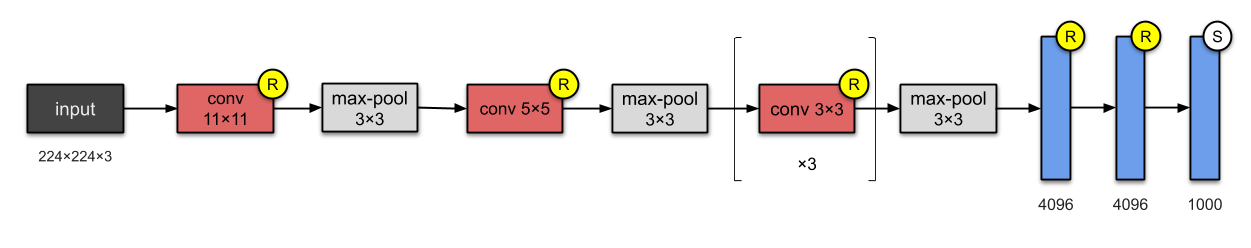
\includegraphics{wiki/1_d_1.png}
\caption{alex net arch}
\end{figure}

Convolution layers in both networks almost have same amount of
parameters and because \emph{Inception V1} a.k.a. \emph{GoogLeNet} has
more conv layers, it has more parameters excluding fully connected
parts.

In term of convolution parameters: 1. Inception: 3.2M 2. AlexNet: 2.5M

But what makes this huge difference is the connection between conv
layers and fully connected layers and also the connection between fully
connected layers itself.

In \emph{AlexNet}, the connection between last pooling layer and first
fully connected layer has about 37M parameters and on top of it, the
connection between this layer and next fully connected layer has 16M
parameters too so only these 2 layers of 8-layer AlexNet have more than
54M parameteres while the entire \emph{Inception} model has 7M
parameters which has been explained later. Here is an image of last
pooling layer and 2 fully connected layers of \emph{AlexNet}:

\begin{figure}
\centering
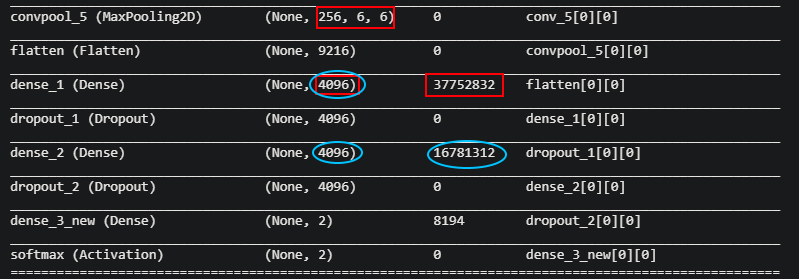
\includegraphics{wiki/1_d_3.png}
\caption{alex net last fcn}
\end{figure}

What about \emph{Inception}? Inception V1:

\begin{figure}
\centering
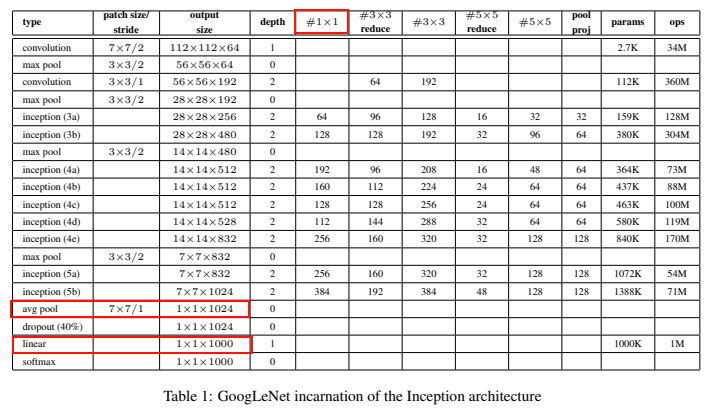
\includegraphics{wiki/1_d_2.png}
\caption{inception v1}
\end{figure}

About \emph{Inception} we need to focus on two procedure: 1.
\texttt{1x1} Convs: As we know in Inception module, different convs have
been taken and then concatnated but before doing this, they first take
\texttt{1v1} conv for sake of dimensionality reduction.

\begin{enumerate}
\def\labelenumi{\arabic{enumi}.}
\setcounter{enumi}{1}
\tightlist
\item
  Using \texttt{GlobalAveragePooling} in the last layer after Inception
  layers helped to reduce the last convotional layer to only 1024, then
  a fully connected with 1000 neurons are connected at the last layer.
\end{enumerate}

Note that there are 2 other auxiliry losses with same logic (after
Inception4a and Inception 4d) so approximately all three pathes have
about 3M parameters + 3.2M parameters of inception modules and other
conv layers, we reach 7M parameters.

\begin{figure}
\centering
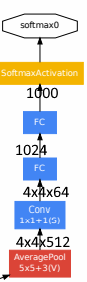
\includegraphics{wiki/1_d_4.png}
\caption{aux loss}
\end{figure}

Image above shows the dimensionality of different layers at the
connection of conv layers to fully connected for auxility loss 1. This
is same for aux loss 2 except tensor after avg pooling is
\texttt{4x4x528} instead of \texttt{4x4x512x}.

Below image also show the main path (main loss) of GoogleNet:

\begin{figure}
\centering
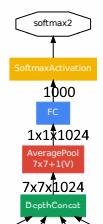
\includegraphics{wiki/1_d_5.png}
\caption{main path}
\end{figure}

    \hypertarget{summarize-xception-model}{%
\subsection{\texorpdfstring{2 Summarize
\href{http://openaccess.thecvf.com/content_cvpr_2017/papers/Chollet_Xception_Deep_Learning_CVPR_2017_paper.pdf}{Xception}
model}{2 Summarize Xception model}}\label{summarize-xception-model}}

\begin{enumerate}
\def\labelenumi{\arabic{enumi}.}
\tightlist
\item
  LeNet
\item
  AlexNet
\item
  VGG
\item
  ResNet
\item
  Inception (GoogleNet)
\item
  Xception
\end{enumerate}

Note: In all modules, circles with \emph{T=Tanh}, \emph{S=Sigmoid} and
\emph{R=ReLU}

    \hypertarget{a-lenet}{%
\subsubsection{2.A LeNet}\label{a-lenet}}

LeNet is simplest neural network here, just 2 conv layer and 3 FCs. This
model has only 0.6M parameters.

\begin{figure}
\centering
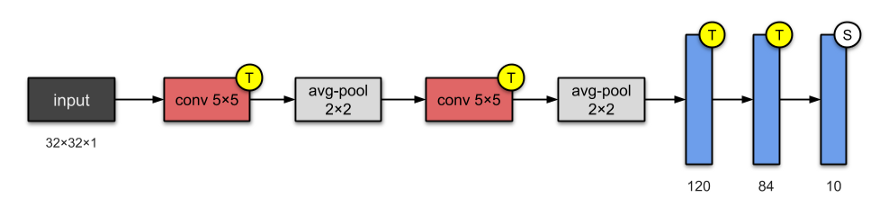
\includegraphics{wiki/2_1.png}
\caption{lenet}
\end{figure}

    \hypertarget{b-alexnet}{%
\subsubsection{2.B AlexNet}\label{b-alexnet}}

AlexNet has 8 layers. What is interesting about this network is that the
idea of stacking multiple convolutions then reducing the spatial size of
filters has been introduced which is commonly used in almost all
networks. The other important note is that they introduced ReLU
activation in this paper.

This model has huge capacity with 60M parameters and at the time of
publishing, implementing this using available GPUs was challenge so they
used parallel implementation of different operation that led them win
challenges.

\begin{figure}
\centering
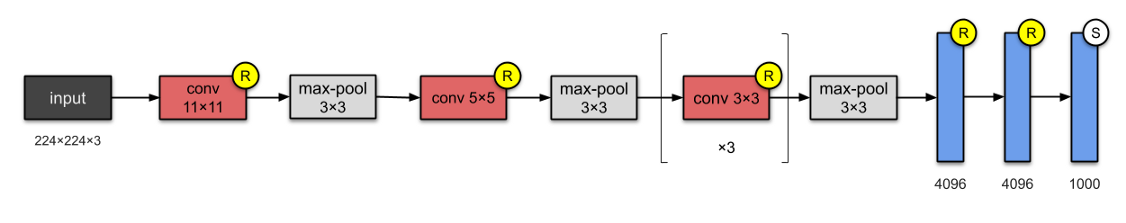
\includegraphics{wiki/2_2.png}
\caption{alex net}
\end{figure}

    \hypertarget{c-vgg}{%
\subsubsection{2.C VGG}\label{c-vgg}}

VGG has two main difference from AlexNet 1. VGG uses smaller filter
sizes like 2x2 or 3x3 instead of using big ones like 11x11 at first then
reduing the filter sizes and reducing volume sizes has been taken care
of by maxpooling layers. 2. VGG is much deeper and the reason is that in
the corresponding paper (or many books) it has been shown that deeper
and bigger neural networks has more capacity to learn, so why not
deeper?!

They stacked much more layers of smaller filter sizes so as we can guess
number of parameters increased to 138M. VGG has different models that a
number follows the name VGG which demonstrates number of layers of
model. Most reknown ones are VGG-16 and VGG-19.

Something is good to know is that in many different tasks, people use
intermediate layers of VGG trained on ImageNet as latent vector of
feature extractor or directly transfering knowledge from VGG model for
their particular tasks.

\begin{figure}
\centering
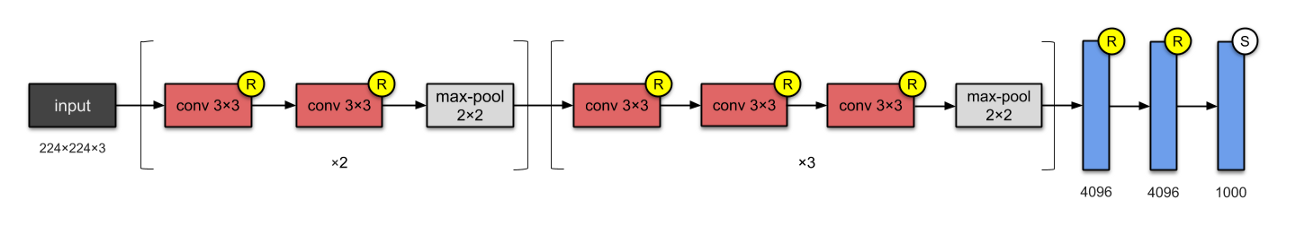
\includegraphics{wiki/2_3.png}
\caption{VGG}
\end{figure}

This one may show much better:

\begin{figure}
\centering
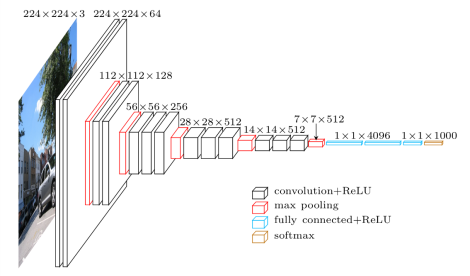
\includegraphics{wiki/2_4.png}
\caption{VGG 2}
\end{figure}

    \hypertarget{d-resnet}{%
\subsubsection{2.D ResNet}\label{d-resnet}}

The resnet's idea is really simple in intuitive way, ``go deeper and
deeper but you might forget what you have learned before, so every time
you go deeper, try to learn new thing, if you cannot, retain what ever
you have had so far (by identity function!)''.

Actually I made up the sentence above but it is absolutely true about
ResNet. Here is an image that helps:

\begin{figure}
\centering
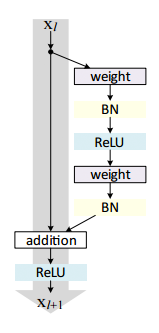
\includegraphics{wiki/2_5.png}
\caption{resnet bottleneck}
\end{figure}

The other parts are similar to any other networks, stacking up multiple
layers but this time, we stack everytime a single one of aforementioned
layers called ResNet block(bottleneck). The straight lines works as
identity function in simplified terms called skipping connections.

This architecture helps scientists to build much deeper networks from 20
layers to nowadays 1000 layers with increase in accuracy by increasing
layers thanks to those micro-architectures(resnet blocks).

Because ResNet also uses global average pooling(we can see similar
effect in Inception module) the number of parameters is much less than
AlexNet. For instance, ResNet-50 with 50 layers has only 26M parameters.

\begin{figure}
\centering
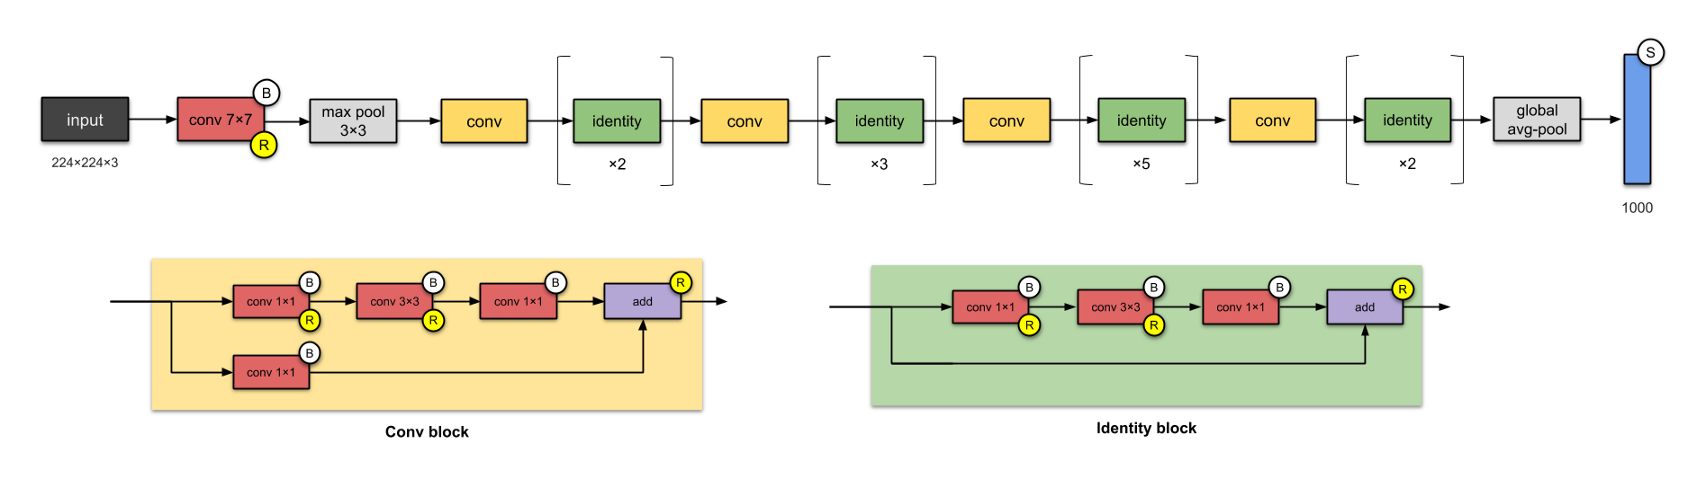
\includegraphics{wiki/2_6.png}
\caption{resnet arch}
\end{figure}

    \hypertarget{e-inception-v1}{%
\subsubsection{2.E Inception-V1}\label{e-inception-v1}}

please see section 1.D

    \hypertarget{f-xception}{%
\subsubsection{2.F Xception}\label{f-xception}}

The first point I would like to focus on is that \emph{Xception} only
not introduces new artichtecture, it also depicts a new approach of
taking convolutions called \emph{Depthwise separable convolutions} which
is enormously faster than normal convolution we knew from other models
such as \emph{ResNet}, \emph{VGG}.

What is \emph{depthwise convolution}? Multiplication is a expensive
operation for computer and in a normal convolution for a image with size
of \texttt{H*H*M} and \texttt{N} filters with size of \texttt{K*K*M},
the number of multiplication will be \texttt{N*(H-K)\^{}2*K\^{}2*M}.

\emph{Depthwise separable convolution} has two steps: 1. Depthwise
convolution: Only applies convolution to a channel at a time rather than
all channels so we need \texttt{M} filter with size of \texttt{K*K*1}
too. The output size of this step will be in size of \texttt{(H-K)\^{}M}
which needs \texttt{M*K\^{}2*(H-K)\^{}2} multiplications. 2. Pointwise
convolution: Linear combination of these layers with a filter with size
of \texttt{1*1*M}. Assume as normal convolution we need \texttt{N}
filters so we can exapnd the idea here too. The output of this step will
be in size of \texttt{N*(H-K)\^{}2} which needs \texttt{N*(H-K)\^{}2*M}
multiplications.

Finally, the speedup is equal to \texttt{(1/N)\ +\ (1/K\^{}2)}.

In summary, we have same ratio for number of parameters too which is big
deal. This image may help to understand the operation:

\begin{figure}
\centering
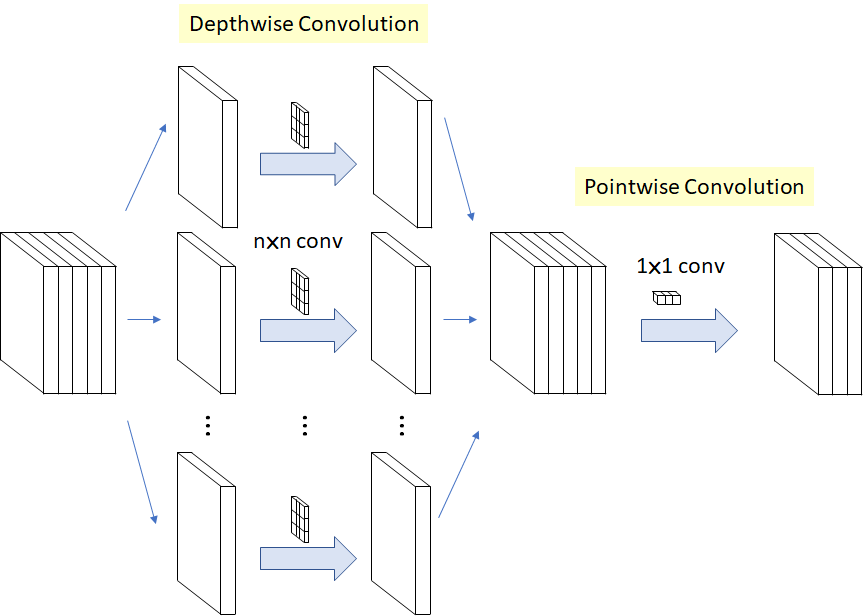
\includegraphics{wiki/3_1.png}
\caption{depthwise separable convoltuions}
\end{figure}

Now we focus on \emph{Xception} module. In \emph{Xception} the order of
operations in depthwise separable convolutions has been reversed which
means first \texttt{1*1} convolutions have been used like below image:

\begin{figure}
\centering
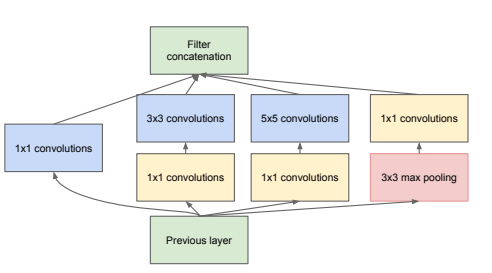
\includegraphics{wiki/3_3.png}
\caption{simplified inception module}
\end{figure}

Xception is the extended version of Inception-V3 (in term of number of
stacked layers) but the main difference as has been explained is using
\emph{depthwize separable convolutions} \emph{eXtreme}ly which is
exactly as the way I have explained in mathematically. The other parts
are very similar to Inception and convetional CNNs.

This model has about 23M parameters.

Here is the final model:

\begin{figure}
\centering
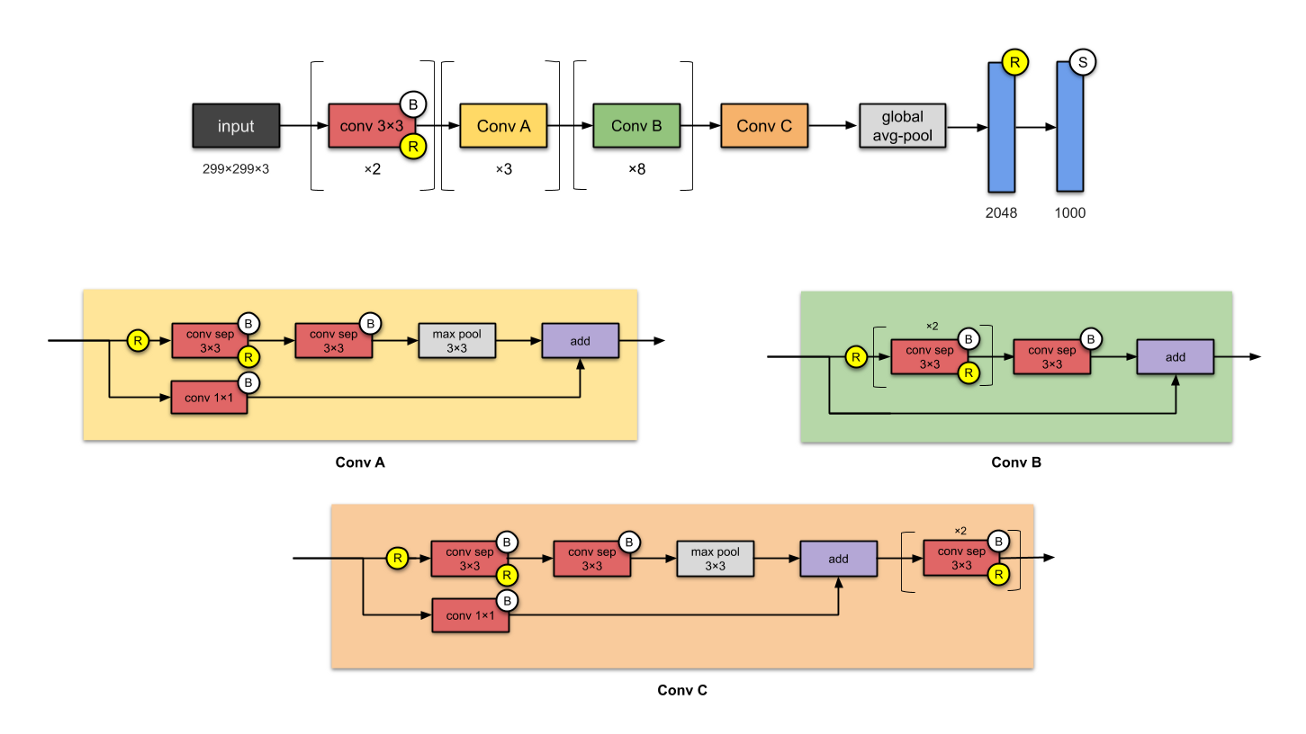
\includegraphics{wiki/2_7.png}
\caption{Xception}
\end{figure}

    \hypertarget{train-a-keras-model-on-cifar10}{%
\subsection{\texorpdfstring{3 Train a \href{https://keras.io/}{Keras}
model on
CIFAR10}{3 Train a Keras model on CIFAR10}}\label{train-a-keras-model-on-cifar10}}

\begin{enumerate}
\def\labelenumi{\arabic{enumi}.}
\tightlist
\item
  Libraries
\item
  Preparing Data

  \begin{enumerate}
  \def\labelenumii{\arabic{enumii}.}
  \tightlist
  \item
    Loading
  \item
    Normalizing
  \item
    Onehot Vector For Labels
  \end{enumerate}
\item
  Setting Hyperparameters
\item
  Learning Rate Decay Callbacks
\item
  Defining ResNet110V2
\item
  Compile Model
\item
  Save Model Callbacks
\item
  Cutout Regularization
\item
  ImageDataGenerator
\item
  Train Model
\item
  Evaluate Model

  \begin{enumerate}
  \def\labelenumii{\arabic{enumii}.}
  \tightlist
  \item
    Last Model
  \item
    Best Model
  \item
    Confusion Matrix of Best Model
  \end{enumerate}
\item
  10 Worst Predictions
\end{enumerate}

    \hypertarget{a-libraries}{%
\subsubsection{3.A Libraries}\label{a-libraries}}

    \begin{Verbatim}[commandchars=\\\{\}]
{\color{incolor}In [{\color{incolor} }]:} \PY{o}{\PYZpc{}}\PY{k}{tensorflow\PYZus{}version} 1.x
        
        \PY{k+kn}{from} \PY{n+nn}{\PYZus{}\PYZus{}future\PYZus{}\PYZus{}} \PY{k}{import} \PY{n}{print\PYZus{}function}   
        \PY{k+kn}{import} \PY{n+nn}{seaborn} \PY{k}{as} \PY{n+nn}{sns}
        \PY{k+kn}{import} \PY{n+nn}{matplotlib}\PY{n+nn}{.}\PY{n+nn}{pylab} \PY{k}{as} \PY{n+nn}{plt}
        \PY{k+kn}{import} \PY{n+nn}{PIL}
        \PY{k+kn}{import} \PY{n+nn}{pandas} \PY{k}{as} \PY{n+nn}{pd}
        \PY{k+kn}{import} \PY{n+nn}{numpy} \PY{k}{as} \PY{n+nn}{np}
        \PY{k+kn}{from} \PY{n+nn}{keras} \PY{k}{import} \PY{n}{backend} \PY{k}{as} \PY{n}{K}
        \PY{k+kn}{from} \PY{n+nn}{keras}\PY{n+nn}{.}\PY{n+nn}{preprocessing}\PY{n+nn}{.}\PY{n+nn}{image} \PY{k}{import} \PY{n}{ImageDataGenerator}
        \PY{k+kn}{from} \PY{n+nn}{keras}\PY{n+nn}{.}\PY{n+nn}{optimizers} \PY{k}{import} \PY{n}{Adam}
        \PY{k+kn}{from} \PY{n+nn}{keras}\PY{n+nn}{.}\PY{n+nn}{callbacks} \PY{k}{import} \PY{n}{EarlyStopping}\PY{p}{,} \PY{n}{ReduceLROnPlateau}\PY{p}{,} \PY{n}{ModelCheckpoint}\PY{p}{,} \PY{n}{LearningRateScheduler}
        \PY{k+kn}{from} \PY{n+nn}{keras}\PY{n+nn}{.}\PY{n+nn}{layers} \PY{k}{import} \PY{n}{Dense}\PY{p}{,} \PY{n}{Conv2D}\PY{p}{,} \PY{n}{BatchNormalization}\PY{p}{,} \PY{n}{Activation}
        \PY{k+kn}{from} \PY{n+nn}{keras}\PY{n+nn}{.}\PY{n+nn}{layers} \PY{k}{import} \PY{n}{AveragePooling2D}\PY{p}{,} \PY{n}{Input}\PY{p}{,} \PY{n}{Flatten}
        \PY{k+kn}{from} \PY{n+nn}{keras}\PY{n+nn}{.}\PY{n+nn}{regularizers} \PY{k}{import} \PY{n}{l2}
        \PY{k+kn}{from} \PY{n+nn}{keras}\PY{n+nn}{.}\PY{n+nn}{models} \PY{k}{import} \PY{n}{Model}
        \PY{k+kn}{from} \PY{n+nn}{keras}\PY{n+nn}{.}\PY{n+nn}{utils} \PY{k}{import} \PY{n}{to\PYZus{}categorical}
        \PY{k+kn}{import} \PY{n+nn}{keras}
        
        \PY{k+kn}{from} \PY{n+nn}{keras}\PY{n+nn}{.}\PY{n+nn}{datasets} \PY{k}{import} \PY{n}{cifar10} 
\end{Verbatim}


    \hypertarget{b-preparing-data}{%
\subsubsection{3.B Preparing Data}\label{b-preparing-data}}

\begin{enumerate}
\def\labelenumi{\arabic{enumi}.}
\tightlist
\item
  loading
\item
  normalizing
\item
  converting labels to onehot vectors
\end{enumerate}

    \hypertarget{b.a-loading}{%
\paragraph{3.B.a Loading}\label{b.a-loading}}

    \begin{Verbatim}[commandchars=\\\{\}]
{\color{incolor}In [{\color{incolor}5}]:} \PY{p}{(}\PY{n}{x\PYZus{}train}\PY{p}{,} \PY{n}{y\PYZus{}train}\PY{p}{)}\PY{p}{,} \PY{p}{(}\PY{n}{x\PYZus{}test}\PY{p}{,} \PY{n}{y\PYZus{}test}\PY{p}{)} \PY{o}{=} \PY{n}{cifar10}\PY{o}{.}\PY{n}{load\PYZus{}data}\PY{p}{(}\PY{p}{)}
\end{Verbatim}


    \begin{Verbatim}[commandchars=\\\{\}]
Downloading data from https://www.cs.toronto.edu/\textasciitilde{}kriz/cifar-10-python.tar.gz
170500096/170498071 [==============================] - 4s 0us/step

    \end{Verbatim}

    \hypertarget{b.b-normalizing}{%
\paragraph{3.B.b Normalizing}\label{b.b-normalizing}}

    \begin{Verbatim}[commandchars=\\\{\}]
{\color{incolor}In [{\color{incolor}6}]:} \PY{n}{x\PYZus{}train} \PY{o}{=} \PY{n}{x\PYZus{}train}\PY{o}{.}\PY{n}{astype}\PY{p}{(}\PY{l+s+s1}{\PYZsq{}}\PY{l+s+s1}{float32}\PY{l+s+s1}{\PYZsq{}}\PY{p}{)} \PY{o}{/} \PY{l+m+mi}{255}
        \PY{n}{x\PYZus{}test} \PY{o}{=} \PY{n}{x\PYZus{}test}\PY{o}{.}\PY{n}{astype}\PY{p}{(}\PY{l+s+s1}{\PYZsq{}}\PY{l+s+s1}{float32}\PY{l+s+s1}{\PYZsq{}}\PY{p}{)} \PY{o}{/} \PY{l+m+mi}{255}
        \PY{n}{x\PYZus{}train\PYZus{}mean} \PY{o}{=} \PY{n}{np}\PY{o}{.}\PY{n}{mean}\PY{p}{(}\PY{n}{x\PYZus{}train}\PY{p}{,} \PY{n}{axis}\PY{o}{=}\PY{l+m+mi}{0}\PY{p}{)}
        \PY{n}{x\PYZus{}train} \PY{o}{\PYZhy{}}\PY{o}{=} \PY{n}{x\PYZus{}train\PYZus{}mean}
        \PY{n}{x\PYZus{}test} \PY{o}{\PYZhy{}}\PY{o}{=} \PY{n}{x\PYZus{}train\PYZus{}mean}
        
        \PY{n+nb}{print}\PY{p}{(}\PY{l+s+s1}{\PYZsq{}}\PY{l+s+s1}{x\PYZus{}train shape:}\PY{l+s+s1}{\PYZsq{}}\PY{p}{,} \PY{n}{x\PYZus{}train}\PY{o}{.}\PY{n}{shape}\PY{p}{)}
        \PY{n+nb}{print}\PY{p}{(}\PY{l+s+s1}{\PYZsq{}}\PY{l+s+s1}{train samples}\PY{l+s+s1}{\PYZsq{}}\PY{p}{,} \PY{n}{x\PYZus{}train}\PY{o}{.}\PY{n}{shape}\PY{p}{[}\PY{l+m+mi}{0}\PY{p}{]}\PY{p}{)}
        \PY{n+nb}{print}\PY{p}{(}\PY{l+s+s1}{\PYZsq{}}\PY{l+s+s1}{test samples}\PY{l+s+s1}{\PYZsq{}}\PY{p}{,} \PY{n}{x\PYZus{}test}\PY{o}{.}\PY{n}{shape}\PY{p}{[}\PY{l+m+mi}{0}\PY{p}{]}\PY{p}{)}
        \PY{n+nb}{print}\PY{p}{(}\PY{l+s+s1}{\PYZsq{}}\PY{l+s+s1}{y\PYZus{}train shape:}\PY{l+s+s1}{\PYZsq{}}\PY{p}{,} \PY{n}{y\PYZus{}train}\PY{o}{.}\PY{n}{shape}\PY{p}{)}
\end{Verbatim}


    \begin{Verbatim}[commandchars=\\\{\}]
x\_train shape: (50000, 32, 32, 3)
train samples 50000
test samples 10000
y\_train shape: (50000, 1)

    \end{Verbatim}

    \hypertarget{b.c-convert-y-to-onehot-vectors}{%
\paragraph{3.B.c Convert Y to onehot
vectors}\label{b.c-convert-y-to-onehot-vectors}}

    \begin{Verbatim}[commandchars=\\\{\}]
{\color{incolor}In [{\color{incolor}8}]:} \PY{n}{num\PYZus{}classes} \PY{o}{=} \PY{l+m+mi}{10}
        \PY{n}{y\PYZus{}train} \PY{o}{=} \PY{n}{to\PYZus{}categorical}\PY{p}{(}\PY{n}{y\PYZus{}train}\PY{p}{,} \PY{n}{num\PYZus{}classes}\PY{p}{)}
        \PY{n}{y\PYZus{}test} \PY{o}{=} \PY{n}{to\PYZus{}categorical}\PY{p}{(}\PY{n}{y\PYZus{}test}\PY{p}{,} \PY{n}{num\PYZus{}classes}\PY{p}{)}
        \PY{n+nb}{print}\PY{p}{(}\PY{n}{y\PYZus{}train}\PY{o}{.}\PY{n}{shape}\PY{p}{)}
\end{Verbatim}


    \begin{Verbatim}[commandchars=\\\{\}]
(50000, 10)

    \end{Verbatim}

    \hypertarget{c-setting-hyperparameters}{%
\subsubsection{3.C Setting
Hyperparameters}\label{c-setting-hyperparameters}}

    \begin{Verbatim}[commandchars=\\\{\}]
{\color{incolor}In [{\color{incolor} }]:} \PY{n}{batch\PYZus{}size} \PY{o}{=} \PY{l+m+mi}{32}
        \PY{n}{epochs} \PY{o}{=} \PY{l+m+mi}{200}
        
        \PY{n}{data\PYZus{}augmentation} \PY{o}{=} \PY{k+kc}{True}
        \PY{n}{subtract\PYZus{}pixel\PYZus{}mean} \PY{o}{=} \PY{k+kc}{True}
        
        \PY{c+c1}{\PYZsh{} resnet 110 v2}
        \PY{n}{depth} \PY{o}{=} \PY{l+m+mi}{110}  
        \PY{n}{version} \PY{o}{=} \PY{l+m+mi}{2} 
        \PY{n}{model\PYZus{}type} \PY{o}{=} \PY{l+s+s1}{\PYZsq{}}\PY{l+s+s1}{ResNet110v2}\PY{l+s+s1}{\PYZsq{}}
\end{Verbatim}


    \begin{Verbatim}[commandchars=\\\{\}]
{\color{incolor}In [{\color{incolor} }]:} \PY{n}{input\PYZus{}shape} \PY{o}{=} \PY{n}{x\PYZus{}train}\PY{o}{.}\PY{n}{shape}\PY{p}{[}\PY{l+m+mi}{1}\PY{p}{:}\PY{p}{]}
\end{Verbatim}


    \hypertarget{d-learning-rate-decay-callbacks}{%
\subsubsection{3.D Learning Rate Decay
Callbacks}\label{d-learning-rate-decay-callbacks}}

    \begin{Verbatim}[commandchars=\\\{\}]
{\color{incolor}In [{\color{incolor} }]:} \PY{k}{def} \PY{n+nf}{lr\PYZus{}schedule}\PY{p}{(}\PY{n}{epoch}\PY{p}{)}\PY{p}{:}
            \PY{l+s+sd}{\PYZdq{}\PYZdq{}\PYZdq{}}
        \PY{l+s+sd}{    Learning Rate Schedule}
        
        \PY{l+s+sd}{    Learning rate is scheduled to be reduced after 80, 120, 160, 180 epochs.}
        \PY{l+s+sd}{    Called automatically every epoch as part of callbacks during training.}
        
        \PY{l+s+sd}{    }
        \PY{l+s+sd}{    :param epoch: The number of epochs}
        
        \PY{l+s+sd}{    :Returns: lr (float32) learning rate}
        \PY{l+s+sd}{    \PYZdq{}\PYZdq{}\PYZdq{}}
            \PY{n}{lr} \PY{o}{=} \PY{l+m+mf}{1e\PYZhy{}3}
            \PY{k}{if} \PY{n}{epoch} \PY{o}{\PYZgt{}} \PY{l+m+mi}{180}\PY{p}{:}
                \PY{n}{lr} \PY{o}{*}\PY{o}{=} \PY{l+m+mf}{0.5e\PYZhy{}3}
            \PY{k}{elif} \PY{n}{epoch} \PY{o}{\PYZgt{}} \PY{l+m+mi}{160}\PY{p}{:}
                \PY{n}{lr} \PY{o}{*}\PY{o}{=} \PY{l+m+mf}{1e\PYZhy{}3}
            \PY{k}{elif} \PY{n}{epoch} \PY{o}{\PYZgt{}} \PY{l+m+mi}{120}\PY{p}{:}
                \PY{n}{lr} \PY{o}{*}\PY{o}{=} \PY{l+m+mf}{1e\PYZhy{}2}
            \PY{k}{elif} \PY{n}{epoch} \PY{o}{\PYZgt{}} \PY{l+m+mi}{80}\PY{p}{:}
                \PY{n}{lr} \PY{o}{*}\PY{o}{=} \PY{l+m+mf}{1e\PYZhy{}1}
            \PY{n+nb}{print}\PY{p}{(}\PY{l+s+s1}{\PYZsq{}}\PY{l+s+s1}{Learning rate: }\PY{l+s+s1}{\PYZsq{}}\PY{p}{,} \PY{n}{lr}\PY{p}{)}
            \PY{k}{return} \PY{n}{lr}
        
        
        \PY{n}{lr\PYZus{}scheduler} \PY{o}{=} \PY{n}{LearningRateScheduler}\PY{p}{(}\PY{n}{lr\PYZus{}schedule}\PY{p}{)}
        \PY{n}{lr\PYZus{}reducer} \PY{o}{=} \PY{n}{ReduceLROnPlateau}\PY{p}{(}\PY{n}{factor}\PY{o}{=}\PY{n}{np}\PY{o}{.}\PY{n}{sqrt}\PY{p}{(}\PY{l+m+mf}{0.1}\PY{p}{)}\PY{p}{,} \PY{n}{cooldown}\PY{o}{=}\PY{l+m+mi}{0}\PY{p}{,} \PY{n}{patience}\PY{o}{=}\PY{l+m+mi}{5}\PY{p}{,} \PY{n}{min\PYZus{}lr}\PY{o}{=}\PY{l+m+mf}{0.5e\PYZhy{}6}\PY{p}{)}
\end{Verbatim}


    \hypertarget{e-defining-resnet110v2}{%
\subsubsection{3.E Defining ResNet110V2}\label{e-defining-resnet110v2}}

    \begin{Verbatim}[commandchars=\\\{\}]
{\color{incolor}In [{\color{incolor} }]:} \PY{k}{def} \PY{n+nf}{resnet\PYZus{}layer}\PY{p}{(}\PY{n}{inputs}\PY{p}{,} \PY{n}{num\PYZus{}filters}\PY{o}{=}\PY{l+m+mi}{16}\PY{p}{,} \PY{n}{kernel\PYZus{}size}\PY{o}{=}\PY{l+m+mi}{3}\PY{p}{,} \PY{n}{strides}\PY{o}{=}\PY{l+m+mi}{1}\PY{p}{,} \PY{n}{activation}\PY{o}{=}\PY{l+s+s1}{\PYZsq{}}\PY{l+s+s1}{relu}\PY{l+s+s1}{\PYZsq{}}\PY{p}{,} \PY{n}{batch\PYZus{}normalization}\PY{o}{=}\PY{k+kc}{True}\PY{p}{,} \PY{n}{conv\PYZus{}first}\PY{o}{=}\PY{k+kc}{True}\PY{p}{)}\PY{p}{:}
            \PY{l+s+sd}{\PYZdq{}\PYZdq{}\PYZdq{}2D Convolution\PYZhy{}Batch Normalization\PYZhy{}Activation block}
        
        \PY{l+s+sd}{    :param inputs (tensor): input tensor from input image or previous layer}
        \PY{l+s+sd}{    :param num\PYZus{}filters (int): Conv2D number of filters}
        \PY{l+s+sd}{    :param kernel\PYZus{}size (int): Conv2D kernel dimensions}
        \PY{l+s+sd}{    :param strides (int): Conv2D stride dimensions}
        \PY{l+s+sd}{    :param activation (string): activation name}
        \PY{l+s+sd}{    :param batch\PYZus{}normalization (bool): whether to include batch normalization}
        \PY{l+s+sd}{    :param conv\PYZus{}first (bool): conv\PYZhy{}bn\PYZhy{}activation (True) or bn\PYZhy{}activation\PYZhy{}conv (False)}
        
        \PY{l+s+sd}{    :return: x (tensor) tensor as input to the next layer}
        \PY{l+s+sd}{    \PYZdq{}\PYZdq{}\PYZdq{}}
            \PY{n}{conv} \PY{o}{=} \PY{n}{Conv2D}\PY{p}{(}\PY{n}{num\PYZus{}filters}\PY{p}{,} \PY{n}{kernel\PYZus{}size}\PY{o}{=}\PY{n}{kernel\PYZus{}size}\PY{p}{,} \PY{n}{strides}\PY{o}{=}\PY{n}{strides}\PY{p}{,} \PY{n}{padding}\PY{o}{=}\PY{l+s+s1}{\PYZsq{}}\PY{l+s+s1}{same}\PY{l+s+s1}{\PYZsq{}}\PY{p}{,} \PY{n}{kernel\PYZus{}initializer}\PY{o}{=}\PY{l+s+s1}{\PYZsq{}}\PY{l+s+s1}{he\PYZus{}normal}\PY{l+s+s1}{\PYZsq{}}\PY{p}{,} \PY{n}{kernel\PYZus{}regularizer}\PY{o}{=}\PY{n}{l2}\PY{p}{(}\PY{l+m+mf}{1e\PYZhy{}4}\PY{p}{)}\PY{p}{)}
        
            \PY{n}{x} \PY{o}{=} \PY{n}{inputs}
            \PY{k}{if} \PY{n}{conv\PYZus{}first}\PY{p}{:}
                \PY{n}{x} \PY{o}{=} \PY{n}{conv}\PY{p}{(}\PY{n}{x}\PY{p}{)}
                \PY{k}{if} \PY{n}{batch\PYZus{}normalization}\PY{p}{:}
                    \PY{n}{x} \PY{o}{=} \PY{n}{BatchNormalization}\PY{p}{(}\PY{p}{)}\PY{p}{(}\PY{n}{x}\PY{p}{)}
                \PY{k}{if} \PY{n}{activation} \PY{o+ow}{is} \PY{o+ow}{not} \PY{k+kc}{None}\PY{p}{:}
                    \PY{n}{x} \PY{o}{=} \PY{n}{Activation}\PY{p}{(}\PY{n}{activation}\PY{p}{)}\PY{p}{(}\PY{n}{x}\PY{p}{)}
            \PY{k}{else}\PY{p}{:}
                \PY{k}{if} \PY{n}{batch\PYZus{}normalization}\PY{p}{:}
                    \PY{n}{x} \PY{o}{=} \PY{n}{BatchNormalization}\PY{p}{(}\PY{p}{)}\PY{p}{(}\PY{n}{x}\PY{p}{)}
                \PY{k}{if} \PY{n}{activation} \PY{o+ow}{is} \PY{o+ow}{not} \PY{k+kc}{None}\PY{p}{:}
                    \PY{n}{x} \PY{o}{=} \PY{n}{Activation}\PY{p}{(}\PY{n}{activation}\PY{p}{)}\PY{p}{(}\PY{n}{x}\PY{p}{)}
                \PY{n}{x} \PY{o}{=} \PY{n}{conv}\PY{p}{(}\PY{n}{x}\PY{p}{)}
            \PY{k}{return} \PY{n}{x}
        
        
        
        \PY{k}{def} \PY{n+nf}{resnet110v2}\PY{p}{(}\PY{n}{input\PYZus{}shape}\PY{p}{,} \PY{n}{num\PYZus{}classes}\PY{o}{=}\PY{l+m+mi}{10}\PY{p}{)}\PY{p}{:}
            \PY{l+s+sd}{\PYZdq{}\PYZdq{}\PYZdq{}}
        \PY{l+s+sd}{    ResNet Version 2 Model}
        
        \PY{l+s+sd}{    Stacks of (1 x 1)\PYZhy{}(3 x 3)\PYZhy{}(1 x 1) BN\PYZhy{}ReLU\PYZhy{}Conv2D}
        \PY{l+s+sd}{    First shortcut connection per layer is 1 x 1 Conv2D.}
        \PY{l+s+sd}{    Second and onwards shortcut connection is identity.}
        \PY{l+s+sd}{    At the beginning of each stage, the feature map size is halved (downsampled)}
        \PY{l+s+sd}{    by a convolutional layer with strides=2, while the number of filter maps is}
        \PY{l+s+sd}{    doubled. Within each stage, the layers have the same number filters and the}
        \PY{l+s+sd}{    same filter map sizes.}
        \PY{l+s+sd}{    Features maps sizes:}
        \PY{l+s+sd}{    conv1  : 32x32,  16}
        \PY{l+s+sd}{    stage 0: 32x32,  64}
        \PY{l+s+sd}{    stage 1: 16x16, 128}
        \PY{l+s+sd}{    stage 2:  8x8,  256}
        
        \PY{l+s+sd}{    :param input\PYZus{}shape (tensor): shape of input tensor}
        \PY{l+s+sd}{    :param num\PYZus{}classes (int): number of classes}
        
        \PY{l+s+sd}{    }
        \PY{l+s+sd}{    :return: Keras model instance}
        \PY{l+s+sd}{    \PYZdq{}\PYZdq{}\PYZdq{}}
        
            \PY{c+c1}{\PYZsh{} Start model definition.}
            \PY{n}{num\PYZus{}filters\PYZus{}in} \PY{o}{=} \PY{l+m+mi}{16}
            \PY{n}{num\PYZus{}res\PYZus{}blocks} \PY{o}{=} \PY{l+m+mi}{12}
        
            \PY{n}{inputs} \PY{o}{=} \PY{n}{Input}\PY{p}{(}\PY{n}{shape}\PY{o}{=}\PY{n}{input\PYZus{}shape}\PY{p}{)}
        
            \PY{n}{x} \PY{o}{=} \PY{n}{resnet\PYZus{}layer}\PY{p}{(}\PY{n}{inputs}\PY{o}{=}\PY{n}{inputs}\PY{p}{,} \PY{n}{num\PYZus{}filters}\PY{o}{=}\PY{n}{num\PYZus{}filters\PYZus{}in}\PY{p}{,} \PY{n}{conv\PYZus{}first}\PY{o}{=}\PY{k+kc}{True}\PY{p}{)}
        
            \PY{c+c1}{\PYZsh{} Instantiate the resnet blocks}
            \PY{k}{for} \PY{n}{stage} \PY{o+ow}{in} \PY{n+nb}{range}\PY{p}{(}\PY{l+m+mi}{3}\PY{p}{)}\PY{p}{:}
                \PY{k}{for} \PY{n}{res\PYZus{}block} \PY{o+ow}{in} \PY{n+nb}{range}\PY{p}{(}\PY{n}{num\PYZus{}res\PYZus{}blocks}\PY{p}{)}\PY{p}{:}
                    \PY{n}{activation} \PY{o}{=} \PY{l+s+s1}{\PYZsq{}}\PY{l+s+s1}{relu}\PY{l+s+s1}{\PYZsq{}}
                    \PY{n}{batch\PYZus{}normalization} \PY{o}{=} \PY{k+kc}{True}
                    \PY{n}{strides} \PY{o}{=} \PY{l+m+mi}{1}
                    \PY{k}{if} \PY{n}{stage} \PY{o}{==} \PY{l+m+mi}{0}\PY{p}{:}
                        \PY{n}{num\PYZus{}filters\PYZus{}out} \PY{o}{=} \PY{n}{num\PYZus{}filters\PYZus{}in} \PY{o}{*} \PY{l+m+mi}{4}
                        \PY{k}{if} \PY{n}{res\PYZus{}block} \PY{o}{==} \PY{l+m+mi}{0}\PY{p}{:}  \PY{c+c1}{\PYZsh{} first layer and first stage}
                            \PY{n}{activation} \PY{o}{=} \PY{k+kc}{None}
                            \PY{n}{batch\PYZus{}normalization} \PY{o}{=} \PY{k+kc}{False}
                    \PY{k}{else}\PY{p}{:}
                        \PY{n}{num\PYZus{}filters\PYZus{}out} \PY{o}{=} \PY{n}{num\PYZus{}filters\PYZus{}in} \PY{o}{*} \PY{l+m+mi}{2}
                        \PY{k}{if} \PY{n}{res\PYZus{}block} \PY{o}{==} \PY{l+m+mi}{0}\PY{p}{:}  \PY{c+c1}{\PYZsh{} first layer but not first stage}
                            \PY{n}{strides} \PY{o}{=} \PY{l+m+mi}{2}
        
                    \PY{c+c1}{\PYZsh{} resnet blocks}
                    \PY{n}{y} \PY{o}{=} \PY{n}{resnet\PYZus{}layer}\PY{p}{(}\PY{n}{inputs}\PY{o}{=}\PY{n}{x}\PY{p}{,} \PY{n}{num\PYZus{}filters}\PY{o}{=}\PY{n}{num\PYZus{}filters\PYZus{}in}\PY{p}{,} \PY{n}{kernel\PYZus{}size}\PY{o}{=}\PY{l+m+mi}{1}\PY{p}{,} \PY{n}{strides}\PY{o}{=}\PY{n}{strides}\PY{p}{,} \PY{n}{activation}\PY{o}{=}\PY{n}{activation}\PY{p}{,} 
                                     \PY{n}{batch\PYZus{}normalization}\PY{o}{=}\PY{n}{batch\PYZus{}normalization}\PY{p}{,} \PY{n}{conv\PYZus{}first}\PY{o}{=}\PY{k+kc}{False}\PY{p}{)}
                    \PY{n}{y} \PY{o}{=} \PY{n}{resnet\PYZus{}layer}\PY{p}{(}\PY{n}{inputs}\PY{o}{=}\PY{n}{y}\PY{p}{,} \PY{n}{num\PYZus{}filters}\PY{o}{=}\PY{n}{num\PYZus{}filters\PYZus{}in}\PY{p}{,} \PY{n}{conv\PYZus{}first}\PY{o}{=}\PY{k+kc}{False}\PY{p}{)}
                    \PY{n}{y} \PY{o}{=} \PY{n}{resnet\PYZus{}layer}\PY{p}{(}\PY{n}{inputs}\PY{o}{=}\PY{n}{y}\PY{p}{,} \PY{n}{num\PYZus{}filters}\PY{o}{=}\PY{n}{num\PYZus{}filters\PYZus{}out}\PY{p}{,} \PY{n}{kernel\PYZus{}size}\PY{o}{=}\PY{l+m+mi}{1}\PY{p}{,} \PY{n}{conv\PYZus{}first}\PY{o}{=}\PY{k+kc}{False}\PY{p}{)}
                    \PY{k}{if} \PY{n}{res\PYZus{}block} \PY{o}{==} \PY{l+m+mi}{0}\PY{p}{:}
                        \PY{c+c1}{\PYZsh{} linear projection residual shortcut connection to match}
                        \PY{n}{x} \PY{o}{=} \PY{n}{resnet\PYZus{}layer}\PY{p}{(}\PY{n}{inputs}\PY{o}{=}\PY{n}{x}\PY{p}{,} \PY{n}{num\PYZus{}filters}\PY{o}{=}\PY{n}{num\PYZus{}filters\PYZus{}out}\PY{p}{,} \PY{n}{kernel\PYZus{}size}\PY{o}{=}\PY{l+m+mi}{1}\PY{p}{,} \PY{n}{strides}\PY{o}{=}\PY{n}{strides}\PY{p}{,} \PY{n}{activation}\PY{o}{=}\PY{k+kc}{None}\PY{p}{,} \PY{n}{batch\PYZus{}normalization}\PY{o}{=}\PY{k+kc}{False}\PY{p}{)}
                    \PY{n}{x} \PY{o}{=} \PY{n}{keras}\PY{o}{.}\PY{n}{layers}\PY{o}{.}\PY{n}{add}\PY{p}{(}\PY{p}{[}\PY{n}{x}\PY{p}{,} \PY{n}{y}\PY{p}{]}\PY{p}{)}
        
                \PY{n}{num\PYZus{}filters\PYZus{}in} \PY{o}{=} \PY{n}{num\PYZus{}filters\PYZus{}out}
        
            \PY{c+c1}{\PYZsh{} add classifier}
            \PY{n}{x} \PY{o}{=} \PY{n}{BatchNormalization}\PY{p}{(}\PY{p}{)}\PY{p}{(}\PY{n}{x}\PY{p}{)}
            \PY{n}{x} \PY{o}{=} \PY{n}{Activation}\PY{p}{(}\PY{l+s+s1}{\PYZsq{}}\PY{l+s+s1}{relu}\PY{l+s+s1}{\PYZsq{}}\PY{p}{)}\PY{p}{(}\PY{n}{x}\PY{p}{)}
            \PY{n}{x} \PY{o}{=} \PY{n}{AveragePooling2D}\PY{p}{(}\PY{n}{pool\PYZus{}size}\PY{o}{=}\PY{l+m+mi}{8}\PY{p}{)}\PY{p}{(}\PY{n}{x}\PY{p}{)}
            \PY{n}{y} \PY{o}{=} \PY{n}{Flatten}\PY{p}{(}\PY{p}{)}\PY{p}{(}\PY{n}{x}\PY{p}{)}
            \PY{n}{outputs} \PY{o}{=} \PY{n}{Dense}\PY{p}{(}\PY{n}{num\PYZus{}classes}\PY{p}{,} \PY{n}{activation}\PY{o}{=}\PY{l+s+s1}{\PYZsq{}}\PY{l+s+s1}{softmax}\PY{l+s+s1}{\PYZsq{}}\PY{p}{,} \PY{n}{kernel\PYZus{}initializer}\PY{o}{=}\PY{l+s+s1}{\PYZsq{}}\PY{l+s+s1}{he\PYZus{}normal}\PY{l+s+s1}{\PYZsq{}}\PY{p}{)}\PY{p}{(}\PY{n}{y}\PY{p}{)}
        
            \PY{c+c1}{\PYZsh{} instantiate model}
            \PY{n}{model} \PY{o}{=} \PY{n}{Model}\PY{p}{(}\PY{n}{inputs}\PY{o}{=}\PY{n}{inputs}\PY{p}{,} \PY{n}{outputs}\PY{o}{=}\PY{n}{outputs}\PY{p}{)}
            \PY{k}{return} \PY{n}{model}
\end{Verbatim}


    \hypertarget{f-compile-model}{%
\subsubsection{3.F Compile Model}\label{f-compile-model}}

    \begin{Verbatim}[commandchars=\\\{\}]
{\color{incolor}In [{\color{incolor} }]:} \PY{n}{model} \PY{o}{=} \PY{n}{resnet110v2}\PY{p}{(}\PY{n}{input\PYZus{}shape}\PY{o}{=}\PY{n}{input\PYZus{}shape}\PY{p}{)}
        \PY{n}{model}\PY{o}{.}\PY{n}{compile}\PY{p}{(}\PY{n}{loss}\PY{o}{=}\PY{l+s+s1}{\PYZsq{}}\PY{l+s+s1}{categorical\PYZus{}crossentropy}\PY{l+s+s1}{\PYZsq{}}\PY{p}{,} \PY{n}{optimizer}\PY{o}{=}\PY{n}{Adam}\PY{p}{(}\PY{n}{lr}\PY{o}{=}\PY{n}{lr\PYZus{}schedule}\PY{p}{(}\PY{l+m+mi}{0}\PY{p}{)}\PY{p}{)}\PY{p}{,} \PY{n}{metrics}\PY{o}{=}\PY{p}{[}\PY{l+s+s1}{\PYZsq{}}\PY{l+s+s1}{accuracy}\PY{l+s+s1}{\PYZsq{}}\PY{p}{]}\PY{p}{)}
        \PY{n}{model}\PY{o}{.}\PY{n}{summary}\PY{p}{(}\PY{p}{)}
        \PY{n+nb}{print}\PY{p}{(}\PY{n}{model\PYZus{}type}\PY{p}{)}
\end{Verbatim}


    \begin{Verbatim}[commandchars=\\\{\}]
Learning rate:  0.001
Model: "model\_5"
\_\_\_\_\_\_\_\_\_\_\_\_\_\_\_\_\_\_\_\_\_\_\_\_\_\_\_\_\_\_\_\_\_\_\_\_\_\_\_\_\_\_\_\_\_\_\_\_\_\_\_\_\_\_\_\_\_\_\_\_\_\_\_\_\_\_\_\_\_\_\_\_\_\_\_\_\_\_\_\_\_\_\_\_\_\_\_\_\_\_\_\_\_\_\_\_\_\_
Layer (type)                    Output Shape         Param \#     Connected to                     
==================================================================================================
input\_6 (InputLayer)            (None, 32, 32, 3)    0                                            
\_\_\_\_\_\_\_\_\_\_\_\_\_\_\_\_\_\_\_\_\_\_\_\_\_\_\_\_\_\_\_\_\_\_\_\_\_\_\_\_\_\_\_\_\_\_\_\_\_\_\_\_\_\_\_\_\_\_\_\_\_\_\_\_\_\_\_\_\_\_\_\_\_\_\_\_\_\_\_\_\_\_\_\_\_\_\_\_\_\_\_\_\_\_\_\_\_\_
conv2d\_454 (Conv2D)             (None, 32, 32, 16)   448         input\_6[0][0]                    
\_\_\_\_\_\_\_\_\_\_\_\_\_\_\_\_\_\_\_\_\_\_\_\_\_\_\_\_\_\_\_\_\_\_\_\_\_\_\_\_\_\_\_\_\_\_\_\_\_\_\_\_\_\_\_\_\_\_\_\_\_\_\_\_\_\_\_\_\_\_\_\_\_\_\_\_\_\_\_\_\_\_\_\_\_\_\_\_\_\_\_\_\_\_\_\_\_\_
batch\_normalization\_440 (BatchN (None, 32, 32, 16)   64          conv2d\_454[0][0]                 
\_\_\_\_\_\_\_\_\_\_\_\_\_\_\_\_\_\_\_\_\_\_\_\_\_\_\_\_\_\_\_\_\_\_\_\_\_\_\_\_\_\_\_\_\_\_\_\_\_\_\_\_\_\_\_\_\_\_\_\_\_\_\_\_\_\_\_\_\_\_\_\_\_\_\_\_\_\_\_\_\_\_\_\_\_\_\_\_\_\_\_\_\_\_\_\_\_\_
activation\_440 (Activation)     (None, 32, 32, 16)   0           batch\_normalization\_440[0][0]    
\_\_\_\_\_\_\_\_\_\_\_\_\_\_\_\_\_\_\_\_\_\_\_\_\_\_\_\_\_\_\_\_\_\_\_\_\_\_\_\_\_\_\_\_\_\_\_\_\_\_\_\_\_\_\_\_\_\_\_\_\_\_\_\_\_\_\_\_\_\_\_\_\_\_\_\_\_\_\_\_\_\_\_\_\_\_\_\_\_\_\_\_\_\_\_\_\_\_
conv2d\_455 (Conv2D)             (None, 32, 32, 16)   272         activation\_440[0][0]             
\_\_\_\_\_\_\_\_\_\_\_\_\_\_\_\_\_\_\_\_\_\_\_\_\_\_\_\_\_\_\_\_\_\_\_\_\_\_\_\_\_\_\_\_\_\_\_\_\_\_\_\_\_\_\_\_\_\_\_\_\_\_\_\_\_\_\_\_\_\_\_\_\_\_\_\_\_\_\_\_\_\_\_\_\_\_\_\_\_\_\_\_\_\_\_\_\_\_
batch\_normalization\_441 (BatchN (None, 32, 32, 16)   64          conv2d\_455[0][0]                 
\_\_\_\_\_\_\_\_\_\_\_\_\_\_\_\_\_\_\_\_\_\_\_\_\_\_\_\_\_\_\_\_\_\_\_\_\_\_\_\_\_\_\_\_\_\_\_\_\_\_\_\_\_\_\_\_\_\_\_\_\_\_\_\_\_\_\_\_\_\_\_\_\_\_\_\_\_\_\_\_\_\_\_\_\_\_\_\_\_\_\_\_\_\_\_\_\_\_
activation\_441 (Activation)     (None, 32, 32, 16)   0           batch\_normalization\_441[0][0]    
\_\_\_\_\_\_\_\_\_\_\_\_\_\_\_\_\_\_\_\_\_\_\_\_\_\_\_\_\_\_\_\_\_\_\_\_\_\_\_\_\_\_\_\_\_\_\_\_\_\_\_\_\_\_\_\_\_\_\_\_\_\_\_\_\_\_\_\_\_\_\_\_\_\_\_\_\_\_\_\_\_\_\_\_\_\_\_\_\_\_\_\_\_\_\_\_\_\_
conv2d\_456 (Conv2D)             (None, 32, 32, 16)   2320        activation\_441[0][0]             
\_\_\_\_\_\_\_\_\_\_\_\_\_\_\_\_\_\_\_\_\_\_\_\_\_\_\_\_\_\_\_\_\_\_\_\_\_\_\_\_\_\_\_\_\_\_\_\_\_\_\_\_\_\_\_\_\_\_\_\_\_\_\_\_\_\_\_\_\_\_\_\_\_\_\_\_\_\_\_\_\_\_\_\_\_\_\_\_\_\_\_\_\_\_\_\_\_\_
batch\_normalization\_442 (BatchN (None, 32, 32, 16)   64          conv2d\_456[0][0]                 
\_\_\_\_\_\_\_\_\_\_\_\_\_\_\_\_\_\_\_\_\_\_\_\_\_\_\_\_\_\_\_\_\_\_\_\_\_\_\_\_\_\_\_\_\_\_\_\_\_\_\_\_\_\_\_\_\_\_\_\_\_\_\_\_\_\_\_\_\_\_\_\_\_\_\_\_\_\_\_\_\_\_\_\_\_\_\_\_\_\_\_\_\_\_\_\_\_\_
activation\_442 (Activation)     (None, 32, 32, 16)   0           batch\_normalization\_442[0][0]    
\_\_\_\_\_\_\_\_\_\_\_\_\_\_\_\_\_\_\_\_\_\_\_\_\_\_\_\_\_\_\_\_\_\_\_\_\_\_\_\_\_\_\_\_\_\_\_\_\_\_\_\_\_\_\_\_\_\_\_\_\_\_\_\_\_\_\_\_\_\_\_\_\_\_\_\_\_\_\_\_\_\_\_\_\_\_\_\_\_\_\_\_\_\_\_\_\_\_
conv2d\_458 (Conv2D)             (None, 32, 32, 64)   1088        activation\_440[0][0]             
\_\_\_\_\_\_\_\_\_\_\_\_\_\_\_\_\_\_\_\_\_\_\_\_\_\_\_\_\_\_\_\_\_\_\_\_\_\_\_\_\_\_\_\_\_\_\_\_\_\_\_\_\_\_\_\_\_\_\_\_\_\_\_\_\_\_\_\_\_\_\_\_\_\_\_\_\_\_\_\_\_\_\_\_\_\_\_\_\_\_\_\_\_\_\_\_\_\_
conv2d\_457 (Conv2D)             (None, 32, 32, 64)   1088        activation\_442[0][0]             
\_\_\_\_\_\_\_\_\_\_\_\_\_\_\_\_\_\_\_\_\_\_\_\_\_\_\_\_\_\_\_\_\_\_\_\_\_\_\_\_\_\_\_\_\_\_\_\_\_\_\_\_\_\_\_\_\_\_\_\_\_\_\_\_\_\_\_\_\_\_\_\_\_\_\_\_\_\_\_\_\_\_\_\_\_\_\_\_\_\_\_\_\_\_\_\_\_\_
add\_145 (Add)                   (None, 32, 32, 64)   0           conv2d\_458[0][0]                 
                                                                 conv2d\_457[0][0]                 
\_\_\_\_\_\_\_\_\_\_\_\_\_\_\_\_\_\_\_\_\_\_\_\_\_\_\_\_\_\_\_\_\_\_\_\_\_\_\_\_\_\_\_\_\_\_\_\_\_\_\_\_\_\_\_\_\_\_\_\_\_\_\_\_\_\_\_\_\_\_\_\_\_\_\_\_\_\_\_\_\_\_\_\_\_\_\_\_\_\_\_\_\_\_\_\_\_\_
batch\_normalization\_443 (BatchN (None, 32, 32, 64)   256         add\_145[0][0]                    
\_\_\_\_\_\_\_\_\_\_\_\_\_\_\_\_\_\_\_\_\_\_\_\_\_\_\_\_\_\_\_\_\_\_\_\_\_\_\_\_\_\_\_\_\_\_\_\_\_\_\_\_\_\_\_\_\_\_\_\_\_\_\_\_\_\_\_\_\_\_\_\_\_\_\_\_\_\_\_\_\_\_\_\_\_\_\_\_\_\_\_\_\_\_\_\_\_\_
activation\_443 (Activation)     (None, 32, 32, 64)   0           batch\_normalization\_443[0][0]    
\_\_\_\_\_\_\_\_\_\_\_\_\_\_\_\_\_\_\_\_\_\_\_\_\_\_\_\_\_\_\_\_\_\_\_\_\_\_\_\_\_\_\_\_\_\_\_\_\_\_\_\_\_\_\_\_\_\_\_\_\_\_\_\_\_\_\_\_\_\_\_\_\_\_\_\_\_\_\_\_\_\_\_\_\_\_\_\_\_\_\_\_\_\_\_\_\_\_
conv2d\_459 (Conv2D)             (None, 32, 32, 16)   1040        activation\_443[0][0]             
\_\_\_\_\_\_\_\_\_\_\_\_\_\_\_\_\_\_\_\_\_\_\_\_\_\_\_\_\_\_\_\_\_\_\_\_\_\_\_\_\_\_\_\_\_\_\_\_\_\_\_\_\_\_\_\_\_\_\_\_\_\_\_\_\_\_\_\_\_\_\_\_\_\_\_\_\_\_\_\_\_\_\_\_\_\_\_\_\_\_\_\_\_\_\_\_\_\_
batch\_normalization\_444 (BatchN (None, 32, 32, 16)   64          conv2d\_459[0][0]                 
\_\_\_\_\_\_\_\_\_\_\_\_\_\_\_\_\_\_\_\_\_\_\_\_\_\_\_\_\_\_\_\_\_\_\_\_\_\_\_\_\_\_\_\_\_\_\_\_\_\_\_\_\_\_\_\_\_\_\_\_\_\_\_\_\_\_\_\_\_\_\_\_\_\_\_\_\_\_\_\_\_\_\_\_\_\_\_\_\_\_\_\_\_\_\_\_\_\_
activation\_444 (Activation)     (None, 32, 32, 16)   0           batch\_normalization\_444[0][0]    
\_\_\_\_\_\_\_\_\_\_\_\_\_\_\_\_\_\_\_\_\_\_\_\_\_\_\_\_\_\_\_\_\_\_\_\_\_\_\_\_\_\_\_\_\_\_\_\_\_\_\_\_\_\_\_\_\_\_\_\_\_\_\_\_\_\_\_\_\_\_\_\_\_\_\_\_\_\_\_\_\_\_\_\_\_\_\_\_\_\_\_\_\_\_\_\_\_\_
conv2d\_460 (Conv2D)             (None, 32, 32, 16)   2320        activation\_444[0][0]             
\_\_\_\_\_\_\_\_\_\_\_\_\_\_\_\_\_\_\_\_\_\_\_\_\_\_\_\_\_\_\_\_\_\_\_\_\_\_\_\_\_\_\_\_\_\_\_\_\_\_\_\_\_\_\_\_\_\_\_\_\_\_\_\_\_\_\_\_\_\_\_\_\_\_\_\_\_\_\_\_\_\_\_\_\_\_\_\_\_\_\_\_\_\_\_\_\_\_
batch\_normalization\_445 (BatchN (None, 32, 32, 16)   64          conv2d\_460[0][0]                 
\_\_\_\_\_\_\_\_\_\_\_\_\_\_\_\_\_\_\_\_\_\_\_\_\_\_\_\_\_\_\_\_\_\_\_\_\_\_\_\_\_\_\_\_\_\_\_\_\_\_\_\_\_\_\_\_\_\_\_\_\_\_\_\_\_\_\_\_\_\_\_\_\_\_\_\_\_\_\_\_\_\_\_\_\_\_\_\_\_\_\_\_\_\_\_\_\_\_
activation\_445 (Activation)     (None, 32, 32, 16)   0           batch\_normalization\_445[0][0]    
\_\_\_\_\_\_\_\_\_\_\_\_\_\_\_\_\_\_\_\_\_\_\_\_\_\_\_\_\_\_\_\_\_\_\_\_\_\_\_\_\_\_\_\_\_\_\_\_\_\_\_\_\_\_\_\_\_\_\_\_\_\_\_\_\_\_\_\_\_\_\_\_\_\_\_\_\_\_\_\_\_\_\_\_\_\_\_\_\_\_\_\_\_\_\_\_\_\_
conv2d\_461 (Conv2D)             (None, 32, 32, 64)   1088        activation\_445[0][0]             
\_\_\_\_\_\_\_\_\_\_\_\_\_\_\_\_\_\_\_\_\_\_\_\_\_\_\_\_\_\_\_\_\_\_\_\_\_\_\_\_\_\_\_\_\_\_\_\_\_\_\_\_\_\_\_\_\_\_\_\_\_\_\_\_\_\_\_\_\_\_\_\_\_\_\_\_\_\_\_\_\_\_\_\_\_\_\_\_\_\_\_\_\_\_\_\_\_\_
add\_146 (Add)                   (None, 32, 32, 64)   0           add\_145[0][0]                    
                                                                 conv2d\_461[0][0]                 
\_\_\_\_\_\_\_\_\_\_\_\_\_\_\_\_\_\_\_\_\_\_\_\_\_\_\_\_\_\_\_\_\_\_\_\_\_\_\_\_\_\_\_\_\_\_\_\_\_\_\_\_\_\_\_\_\_\_\_\_\_\_\_\_\_\_\_\_\_\_\_\_\_\_\_\_\_\_\_\_\_\_\_\_\_\_\_\_\_\_\_\_\_\_\_\_\_\_
batch\_normalization\_446 (BatchN (None, 32, 32, 64)   256         add\_146[0][0]                    
\_\_\_\_\_\_\_\_\_\_\_\_\_\_\_\_\_\_\_\_\_\_\_\_\_\_\_\_\_\_\_\_\_\_\_\_\_\_\_\_\_\_\_\_\_\_\_\_\_\_\_\_\_\_\_\_\_\_\_\_\_\_\_\_\_\_\_\_\_\_\_\_\_\_\_\_\_\_\_\_\_\_\_\_\_\_\_\_\_\_\_\_\_\_\_\_\_\_
activation\_446 (Activation)     (None, 32, 32, 64)   0           batch\_normalization\_446[0][0]    
\_\_\_\_\_\_\_\_\_\_\_\_\_\_\_\_\_\_\_\_\_\_\_\_\_\_\_\_\_\_\_\_\_\_\_\_\_\_\_\_\_\_\_\_\_\_\_\_\_\_\_\_\_\_\_\_\_\_\_\_\_\_\_\_\_\_\_\_\_\_\_\_\_\_\_\_\_\_\_\_\_\_\_\_\_\_\_\_\_\_\_\_\_\_\_\_\_\_
conv2d\_462 (Conv2D)             (None, 32, 32, 16)   1040        activation\_446[0][0]             
\_\_\_\_\_\_\_\_\_\_\_\_\_\_\_\_\_\_\_\_\_\_\_\_\_\_\_\_\_\_\_\_\_\_\_\_\_\_\_\_\_\_\_\_\_\_\_\_\_\_\_\_\_\_\_\_\_\_\_\_\_\_\_\_\_\_\_\_\_\_\_\_\_\_\_\_\_\_\_\_\_\_\_\_\_\_\_\_\_\_\_\_\_\_\_\_\_\_
batch\_normalization\_447 (BatchN (None, 32, 32, 16)   64          conv2d\_462[0][0]                 
\_\_\_\_\_\_\_\_\_\_\_\_\_\_\_\_\_\_\_\_\_\_\_\_\_\_\_\_\_\_\_\_\_\_\_\_\_\_\_\_\_\_\_\_\_\_\_\_\_\_\_\_\_\_\_\_\_\_\_\_\_\_\_\_\_\_\_\_\_\_\_\_\_\_\_\_\_\_\_\_\_\_\_\_\_\_\_\_\_\_\_\_\_\_\_\_\_\_
activation\_447 (Activation)     (None, 32, 32, 16)   0           batch\_normalization\_447[0][0]    
\_\_\_\_\_\_\_\_\_\_\_\_\_\_\_\_\_\_\_\_\_\_\_\_\_\_\_\_\_\_\_\_\_\_\_\_\_\_\_\_\_\_\_\_\_\_\_\_\_\_\_\_\_\_\_\_\_\_\_\_\_\_\_\_\_\_\_\_\_\_\_\_\_\_\_\_\_\_\_\_\_\_\_\_\_\_\_\_\_\_\_\_\_\_\_\_\_\_
conv2d\_463 (Conv2D)             (None, 32, 32, 16)   2320        activation\_447[0][0]             
\_\_\_\_\_\_\_\_\_\_\_\_\_\_\_\_\_\_\_\_\_\_\_\_\_\_\_\_\_\_\_\_\_\_\_\_\_\_\_\_\_\_\_\_\_\_\_\_\_\_\_\_\_\_\_\_\_\_\_\_\_\_\_\_\_\_\_\_\_\_\_\_\_\_\_\_\_\_\_\_\_\_\_\_\_\_\_\_\_\_\_\_\_\_\_\_\_\_
batch\_normalization\_448 (BatchN (None, 32, 32, 16)   64          conv2d\_463[0][0]                 
\_\_\_\_\_\_\_\_\_\_\_\_\_\_\_\_\_\_\_\_\_\_\_\_\_\_\_\_\_\_\_\_\_\_\_\_\_\_\_\_\_\_\_\_\_\_\_\_\_\_\_\_\_\_\_\_\_\_\_\_\_\_\_\_\_\_\_\_\_\_\_\_\_\_\_\_\_\_\_\_\_\_\_\_\_\_\_\_\_\_\_\_\_\_\_\_\_\_
activation\_448 (Activation)     (None, 32, 32, 16)   0           batch\_normalization\_448[0][0]    
\_\_\_\_\_\_\_\_\_\_\_\_\_\_\_\_\_\_\_\_\_\_\_\_\_\_\_\_\_\_\_\_\_\_\_\_\_\_\_\_\_\_\_\_\_\_\_\_\_\_\_\_\_\_\_\_\_\_\_\_\_\_\_\_\_\_\_\_\_\_\_\_\_\_\_\_\_\_\_\_\_\_\_\_\_\_\_\_\_\_\_\_\_\_\_\_\_\_
conv2d\_464 (Conv2D)             (None, 32, 32, 64)   1088        activation\_448[0][0]             
\_\_\_\_\_\_\_\_\_\_\_\_\_\_\_\_\_\_\_\_\_\_\_\_\_\_\_\_\_\_\_\_\_\_\_\_\_\_\_\_\_\_\_\_\_\_\_\_\_\_\_\_\_\_\_\_\_\_\_\_\_\_\_\_\_\_\_\_\_\_\_\_\_\_\_\_\_\_\_\_\_\_\_\_\_\_\_\_\_\_\_\_\_\_\_\_\_\_
add\_147 (Add)                   (None, 32, 32, 64)   0           add\_146[0][0]                    
                                                                 conv2d\_464[0][0]                 
\_\_\_\_\_\_\_\_\_\_\_\_\_\_\_\_\_\_\_\_\_\_\_\_\_\_\_\_\_\_\_\_\_\_\_\_\_\_\_\_\_\_\_\_\_\_\_\_\_\_\_\_\_\_\_\_\_\_\_\_\_\_\_\_\_\_\_\_\_\_\_\_\_\_\_\_\_\_\_\_\_\_\_\_\_\_\_\_\_\_\_\_\_\_\_\_\_\_
batch\_normalization\_449 (BatchN (None, 32, 32, 64)   256         add\_147[0][0]                    
\_\_\_\_\_\_\_\_\_\_\_\_\_\_\_\_\_\_\_\_\_\_\_\_\_\_\_\_\_\_\_\_\_\_\_\_\_\_\_\_\_\_\_\_\_\_\_\_\_\_\_\_\_\_\_\_\_\_\_\_\_\_\_\_\_\_\_\_\_\_\_\_\_\_\_\_\_\_\_\_\_\_\_\_\_\_\_\_\_\_\_\_\_\_\_\_\_\_
activation\_449 (Activation)     (None, 32, 32, 64)   0           batch\_normalization\_449[0][0]    
\_\_\_\_\_\_\_\_\_\_\_\_\_\_\_\_\_\_\_\_\_\_\_\_\_\_\_\_\_\_\_\_\_\_\_\_\_\_\_\_\_\_\_\_\_\_\_\_\_\_\_\_\_\_\_\_\_\_\_\_\_\_\_\_\_\_\_\_\_\_\_\_\_\_\_\_\_\_\_\_\_\_\_\_\_\_\_\_\_\_\_\_\_\_\_\_\_\_
conv2d\_465 (Conv2D)             (None, 32, 32, 16)   1040        activation\_449[0][0]             
\_\_\_\_\_\_\_\_\_\_\_\_\_\_\_\_\_\_\_\_\_\_\_\_\_\_\_\_\_\_\_\_\_\_\_\_\_\_\_\_\_\_\_\_\_\_\_\_\_\_\_\_\_\_\_\_\_\_\_\_\_\_\_\_\_\_\_\_\_\_\_\_\_\_\_\_\_\_\_\_\_\_\_\_\_\_\_\_\_\_\_\_\_\_\_\_\_\_
batch\_normalization\_450 (BatchN (None, 32, 32, 16)   64          conv2d\_465[0][0]                 
\_\_\_\_\_\_\_\_\_\_\_\_\_\_\_\_\_\_\_\_\_\_\_\_\_\_\_\_\_\_\_\_\_\_\_\_\_\_\_\_\_\_\_\_\_\_\_\_\_\_\_\_\_\_\_\_\_\_\_\_\_\_\_\_\_\_\_\_\_\_\_\_\_\_\_\_\_\_\_\_\_\_\_\_\_\_\_\_\_\_\_\_\_\_\_\_\_\_
activation\_450 (Activation)     (None, 32, 32, 16)   0           batch\_normalization\_450[0][0]    
\_\_\_\_\_\_\_\_\_\_\_\_\_\_\_\_\_\_\_\_\_\_\_\_\_\_\_\_\_\_\_\_\_\_\_\_\_\_\_\_\_\_\_\_\_\_\_\_\_\_\_\_\_\_\_\_\_\_\_\_\_\_\_\_\_\_\_\_\_\_\_\_\_\_\_\_\_\_\_\_\_\_\_\_\_\_\_\_\_\_\_\_\_\_\_\_\_\_
conv2d\_466 (Conv2D)             (None, 32, 32, 16)   2320        activation\_450[0][0]             
\_\_\_\_\_\_\_\_\_\_\_\_\_\_\_\_\_\_\_\_\_\_\_\_\_\_\_\_\_\_\_\_\_\_\_\_\_\_\_\_\_\_\_\_\_\_\_\_\_\_\_\_\_\_\_\_\_\_\_\_\_\_\_\_\_\_\_\_\_\_\_\_\_\_\_\_\_\_\_\_\_\_\_\_\_\_\_\_\_\_\_\_\_\_\_\_\_\_
batch\_normalization\_451 (BatchN (None, 32, 32, 16)   64          conv2d\_466[0][0]                 
\_\_\_\_\_\_\_\_\_\_\_\_\_\_\_\_\_\_\_\_\_\_\_\_\_\_\_\_\_\_\_\_\_\_\_\_\_\_\_\_\_\_\_\_\_\_\_\_\_\_\_\_\_\_\_\_\_\_\_\_\_\_\_\_\_\_\_\_\_\_\_\_\_\_\_\_\_\_\_\_\_\_\_\_\_\_\_\_\_\_\_\_\_\_\_\_\_\_
activation\_451 (Activation)     (None, 32, 32, 16)   0           batch\_normalization\_451[0][0]    
\_\_\_\_\_\_\_\_\_\_\_\_\_\_\_\_\_\_\_\_\_\_\_\_\_\_\_\_\_\_\_\_\_\_\_\_\_\_\_\_\_\_\_\_\_\_\_\_\_\_\_\_\_\_\_\_\_\_\_\_\_\_\_\_\_\_\_\_\_\_\_\_\_\_\_\_\_\_\_\_\_\_\_\_\_\_\_\_\_\_\_\_\_\_\_\_\_\_
conv2d\_467 (Conv2D)             (None, 32, 32, 64)   1088        activation\_451[0][0]             
\_\_\_\_\_\_\_\_\_\_\_\_\_\_\_\_\_\_\_\_\_\_\_\_\_\_\_\_\_\_\_\_\_\_\_\_\_\_\_\_\_\_\_\_\_\_\_\_\_\_\_\_\_\_\_\_\_\_\_\_\_\_\_\_\_\_\_\_\_\_\_\_\_\_\_\_\_\_\_\_\_\_\_\_\_\_\_\_\_\_\_\_\_\_\_\_\_\_
add\_148 (Add)                   (None, 32, 32, 64)   0           add\_147[0][0]                    
                                                                 conv2d\_467[0][0]                 
\_\_\_\_\_\_\_\_\_\_\_\_\_\_\_\_\_\_\_\_\_\_\_\_\_\_\_\_\_\_\_\_\_\_\_\_\_\_\_\_\_\_\_\_\_\_\_\_\_\_\_\_\_\_\_\_\_\_\_\_\_\_\_\_\_\_\_\_\_\_\_\_\_\_\_\_\_\_\_\_\_\_\_\_\_\_\_\_\_\_\_\_\_\_\_\_\_\_
batch\_normalization\_452 (BatchN (None, 32, 32, 64)   256         add\_148[0][0]                    
\_\_\_\_\_\_\_\_\_\_\_\_\_\_\_\_\_\_\_\_\_\_\_\_\_\_\_\_\_\_\_\_\_\_\_\_\_\_\_\_\_\_\_\_\_\_\_\_\_\_\_\_\_\_\_\_\_\_\_\_\_\_\_\_\_\_\_\_\_\_\_\_\_\_\_\_\_\_\_\_\_\_\_\_\_\_\_\_\_\_\_\_\_\_\_\_\_\_
activation\_452 (Activation)     (None, 32, 32, 64)   0           batch\_normalization\_452[0][0]    
\_\_\_\_\_\_\_\_\_\_\_\_\_\_\_\_\_\_\_\_\_\_\_\_\_\_\_\_\_\_\_\_\_\_\_\_\_\_\_\_\_\_\_\_\_\_\_\_\_\_\_\_\_\_\_\_\_\_\_\_\_\_\_\_\_\_\_\_\_\_\_\_\_\_\_\_\_\_\_\_\_\_\_\_\_\_\_\_\_\_\_\_\_\_\_\_\_\_
conv2d\_468 (Conv2D)             (None, 32, 32, 16)   1040        activation\_452[0][0]             
\_\_\_\_\_\_\_\_\_\_\_\_\_\_\_\_\_\_\_\_\_\_\_\_\_\_\_\_\_\_\_\_\_\_\_\_\_\_\_\_\_\_\_\_\_\_\_\_\_\_\_\_\_\_\_\_\_\_\_\_\_\_\_\_\_\_\_\_\_\_\_\_\_\_\_\_\_\_\_\_\_\_\_\_\_\_\_\_\_\_\_\_\_\_\_\_\_\_
batch\_normalization\_453 (BatchN (None, 32, 32, 16)   64          conv2d\_468[0][0]                 
\_\_\_\_\_\_\_\_\_\_\_\_\_\_\_\_\_\_\_\_\_\_\_\_\_\_\_\_\_\_\_\_\_\_\_\_\_\_\_\_\_\_\_\_\_\_\_\_\_\_\_\_\_\_\_\_\_\_\_\_\_\_\_\_\_\_\_\_\_\_\_\_\_\_\_\_\_\_\_\_\_\_\_\_\_\_\_\_\_\_\_\_\_\_\_\_\_\_
activation\_453 (Activation)     (None, 32, 32, 16)   0           batch\_normalization\_453[0][0]    
\_\_\_\_\_\_\_\_\_\_\_\_\_\_\_\_\_\_\_\_\_\_\_\_\_\_\_\_\_\_\_\_\_\_\_\_\_\_\_\_\_\_\_\_\_\_\_\_\_\_\_\_\_\_\_\_\_\_\_\_\_\_\_\_\_\_\_\_\_\_\_\_\_\_\_\_\_\_\_\_\_\_\_\_\_\_\_\_\_\_\_\_\_\_\_\_\_\_
conv2d\_469 (Conv2D)             (None, 32, 32, 16)   2320        activation\_453[0][0]             
\_\_\_\_\_\_\_\_\_\_\_\_\_\_\_\_\_\_\_\_\_\_\_\_\_\_\_\_\_\_\_\_\_\_\_\_\_\_\_\_\_\_\_\_\_\_\_\_\_\_\_\_\_\_\_\_\_\_\_\_\_\_\_\_\_\_\_\_\_\_\_\_\_\_\_\_\_\_\_\_\_\_\_\_\_\_\_\_\_\_\_\_\_\_\_\_\_\_
batch\_normalization\_454 (BatchN (None, 32, 32, 16)   64          conv2d\_469[0][0]                 
\_\_\_\_\_\_\_\_\_\_\_\_\_\_\_\_\_\_\_\_\_\_\_\_\_\_\_\_\_\_\_\_\_\_\_\_\_\_\_\_\_\_\_\_\_\_\_\_\_\_\_\_\_\_\_\_\_\_\_\_\_\_\_\_\_\_\_\_\_\_\_\_\_\_\_\_\_\_\_\_\_\_\_\_\_\_\_\_\_\_\_\_\_\_\_\_\_\_
activation\_454 (Activation)     (None, 32, 32, 16)   0           batch\_normalization\_454[0][0]    
\_\_\_\_\_\_\_\_\_\_\_\_\_\_\_\_\_\_\_\_\_\_\_\_\_\_\_\_\_\_\_\_\_\_\_\_\_\_\_\_\_\_\_\_\_\_\_\_\_\_\_\_\_\_\_\_\_\_\_\_\_\_\_\_\_\_\_\_\_\_\_\_\_\_\_\_\_\_\_\_\_\_\_\_\_\_\_\_\_\_\_\_\_\_\_\_\_\_
conv2d\_470 (Conv2D)             (None, 32, 32, 64)   1088        activation\_454[0][0]             
\_\_\_\_\_\_\_\_\_\_\_\_\_\_\_\_\_\_\_\_\_\_\_\_\_\_\_\_\_\_\_\_\_\_\_\_\_\_\_\_\_\_\_\_\_\_\_\_\_\_\_\_\_\_\_\_\_\_\_\_\_\_\_\_\_\_\_\_\_\_\_\_\_\_\_\_\_\_\_\_\_\_\_\_\_\_\_\_\_\_\_\_\_\_\_\_\_\_
add\_149 (Add)                   (None, 32, 32, 64)   0           add\_148[0][0]                    
                                                                 conv2d\_470[0][0]                 
\_\_\_\_\_\_\_\_\_\_\_\_\_\_\_\_\_\_\_\_\_\_\_\_\_\_\_\_\_\_\_\_\_\_\_\_\_\_\_\_\_\_\_\_\_\_\_\_\_\_\_\_\_\_\_\_\_\_\_\_\_\_\_\_\_\_\_\_\_\_\_\_\_\_\_\_\_\_\_\_\_\_\_\_\_\_\_\_\_\_\_\_\_\_\_\_\_\_
batch\_normalization\_455 (BatchN (None, 32, 32, 64)   256         add\_149[0][0]                    
\_\_\_\_\_\_\_\_\_\_\_\_\_\_\_\_\_\_\_\_\_\_\_\_\_\_\_\_\_\_\_\_\_\_\_\_\_\_\_\_\_\_\_\_\_\_\_\_\_\_\_\_\_\_\_\_\_\_\_\_\_\_\_\_\_\_\_\_\_\_\_\_\_\_\_\_\_\_\_\_\_\_\_\_\_\_\_\_\_\_\_\_\_\_\_\_\_\_
activation\_455 (Activation)     (None, 32, 32, 64)   0           batch\_normalization\_455[0][0]    
\_\_\_\_\_\_\_\_\_\_\_\_\_\_\_\_\_\_\_\_\_\_\_\_\_\_\_\_\_\_\_\_\_\_\_\_\_\_\_\_\_\_\_\_\_\_\_\_\_\_\_\_\_\_\_\_\_\_\_\_\_\_\_\_\_\_\_\_\_\_\_\_\_\_\_\_\_\_\_\_\_\_\_\_\_\_\_\_\_\_\_\_\_\_\_\_\_\_
conv2d\_471 (Conv2D)             (None, 32, 32, 16)   1040        activation\_455[0][0]             
\_\_\_\_\_\_\_\_\_\_\_\_\_\_\_\_\_\_\_\_\_\_\_\_\_\_\_\_\_\_\_\_\_\_\_\_\_\_\_\_\_\_\_\_\_\_\_\_\_\_\_\_\_\_\_\_\_\_\_\_\_\_\_\_\_\_\_\_\_\_\_\_\_\_\_\_\_\_\_\_\_\_\_\_\_\_\_\_\_\_\_\_\_\_\_\_\_\_
batch\_normalization\_456 (BatchN (None, 32, 32, 16)   64          conv2d\_471[0][0]                 
\_\_\_\_\_\_\_\_\_\_\_\_\_\_\_\_\_\_\_\_\_\_\_\_\_\_\_\_\_\_\_\_\_\_\_\_\_\_\_\_\_\_\_\_\_\_\_\_\_\_\_\_\_\_\_\_\_\_\_\_\_\_\_\_\_\_\_\_\_\_\_\_\_\_\_\_\_\_\_\_\_\_\_\_\_\_\_\_\_\_\_\_\_\_\_\_\_\_
activation\_456 (Activation)     (None, 32, 32, 16)   0           batch\_normalization\_456[0][0]    
\_\_\_\_\_\_\_\_\_\_\_\_\_\_\_\_\_\_\_\_\_\_\_\_\_\_\_\_\_\_\_\_\_\_\_\_\_\_\_\_\_\_\_\_\_\_\_\_\_\_\_\_\_\_\_\_\_\_\_\_\_\_\_\_\_\_\_\_\_\_\_\_\_\_\_\_\_\_\_\_\_\_\_\_\_\_\_\_\_\_\_\_\_\_\_\_\_\_
conv2d\_472 (Conv2D)             (None, 32, 32, 16)   2320        activation\_456[0][0]             
\_\_\_\_\_\_\_\_\_\_\_\_\_\_\_\_\_\_\_\_\_\_\_\_\_\_\_\_\_\_\_\_\_\_\_\_\_\_\_\_\_\_\_\_\_\_\_\_\_\_\_\_\_\_\_\_\_\_\_\_\_\_\_\_\_\_\_\_\_\_\_\_\_\_\_\_\_\_\_\_\_\_\_\_\_\_\_\_\_\_\_\_\_\_\_\_\_\_
batch\_normalization\_457 (BatchN (None, 32, 32, 16)   64          conv2d\_472[0][0]                 
\_\_\_\_\_\_\_\_\_\_\_\_\_\_\_\_\_\_\_\_\_\_\_\_\_\_\_\_\_\_\_\_\_\_\_\_\_\_\_\_\_\_\_\_\_\_\_\_\_\_\_\_\_\_\_\_\_\_\_\_\_\_\_\_\_\_\_\_\_\_\_\_\_\_\_\_\_\_\_\_\_\_\_\_\_\_\_\_\_\_\_\_\_\_\_\_\_\_
activation\_457 (Activation)     (None, 32, 32, 16)   0           batch\_normalization\_457[0][0]    
\_\_\_\_\_\_\_\_\_\_\_\_\_\_\_\_\_\_\_\_\_\_\_\_\_\_\_\_\_\_\_\_\_\_\_\_\_\_\_\_\_\_\_\_\_\_\_\_\_\_\_\_\_\_\_\_\_\_\_\_\_\_\_\_\_\_\_\_\_\_\_\_\_\_\_\_\_\_\_\_\_\_\_\_\_\_\_\_\_\_\_\_\_\_\_\_\_\_
conv2d\_473 (Conv2D)             (None, 32, 32, 64)   1088        activation\_457[0][0]             
\_\_\_\_\_\_\_\_\_\_\_\_\_\_\_\_\_\_\_\_\_\_\_\_\_\_\_\_\_\_\_\_\_\_\_\_\_\_\_\_\_\_\_\_\_\_\_\_\_\_\_\_\_\_\_\_\_\_\_\_\_\_\_\_\_\_\_\_\_\_\_\_\_\_\_\_\_\_\_\_\_\_\_\_\_\_\_\_\_\_\_\_\_\_\_\_\_\_
add\_150 (Add)                   (None, 32, 32, 64)   0           add\_149[0][0]                    
                                                                 conv2d\_473[0][0]                 
\_\_\_\_\_\_\_\_\_\_\_\_\_\_\_\_\_\_\_\_\_\_\_\_\_\_\_\_\_\_\_\_\_\_\_\_\_\_\_\_\_\_\_\_\_\_\_\_\_\_\_\_\_\_\_\_\_\_\_\_\_\_\_\_\_\_\_\_\_\_\_\_\_\_\_\_\_\_\_\_\_\_\_\_\_\_\_\_\_\_\_\_\_\_\_\_\_\_
batch\_normalization\_458 (BatchN (None, 32, 32, 64)   256         add\_150[0][0]                    
\_\_\_\_\_\_\_\_\_\_\_\_\_\_\_\_\_\_\_\_\_\_\_\_\_\_\_\_\_\_\_\_\_\_\_\_\_\_\_\_\_\_\_\_\_\_\_\_\_\_\_\_\_\_\_\_\_\_\_\_\_\_\_\_\_\_\_\_\_\_\_\_\_\_\_\_\_\_\_\_\_\_\_\_\_\_\_\_\_\_\_\_\_\_\_\_\_\_
activation\_458 (Activation)     (None, 32, 32, 64)   0           batch\_normalization\_458[0][0]    
\_\_\_\_\_\_\_\_\_\_\_\_\_\_\_\_\_\_\_\_\_\_\_\_\_\_\_\_\_\_\_\_\_\_\_\_\_\_\_\_\_\_\_\_\_\_\_\_\_\_\_\_\_\_\_\_\_\_\_\_\_\_\_\_\_\_\_\_\_\_\_\_\_\_\_\_\_\_\_\_\_\_\_\_\_\_\_\_\_\_\_\_\_\_\_\_\_\_
conv2d\_474 (Conv2D)             (None, 32, 32, 16)   1040        activation\_458[0][0]             
\_\_\_\_\_\_\_\_\_\_\_\_\_\_\_\_\_\_\_\_\_\_\_\_\_\_\_\_\_\_\_\_\_\_\_\_\_\_\_\_\_\_\_\_\_\_\_\_\_\_\_\_\_\_\_\_\_\_\_\_\_\_\_\_\_\_\_\_\_\_\_\_\_\_\_\_\_\_\_\_\_\_\_\_\_\_\_\_\_\_\_\_\_\_\_\_\_\_
batch\_normalization\_459 (BatchN (None, 32, 32, 16)   64          conv2d\_474[0][0]                 
\_\_\_\_\_\_\_\_\_\_\_\_\_\_\_\_\_\_\_\_\_\_\_\_\_\_\_\_\_\_\_\_\_\_\_\_\_\_\_\_\_\_\_\_\_\_\_\_\_\_\_\_\_\_\_\_\_\_\_\_\_\_\_\_\_\_\_\_\_\_\_\_\_\_\_\_\_\_\_\_\_\_\_\_\_\_\_\_\_\_\_\_\_\_\_\_\_\_
activation\_459 (Activation)     (None, 32, 32, 16)   0           batch\_normalization\_459[0][0]    
\_\_\_\_\_\_\_\_\_\_\_\_\_\_\_\_\_\_\_\_\_\_\_\_\_\_\_\_\_\_\_\_\_\_\_\_\_\_\_\_\_\_\_\_\_\_\_\_\_\_\_\_\_\_\_\_\_\_\_\_\_\_\_\_\_\_\_\_\_\_\_\_\_\_\_\_\_\_\_\_\_\_\_\_\_\_\_\_\_\_\_\_\_\_\_\_\_\_
conv2d\_475 (Conv2D)             (None, 32, 32, 16)   2320        activation\_459[0][0]             
\_\_\_\_\_\_\_\_\_\_\_\_\_\_\_\_\_\_\_\_\_\_\_\_\_\_\_\_\_\_\_\_\_\_\_\_\_\_\_\_\_\_\_\_\_\_\_\_\_\_\_\_\_\_\_\_\_\_\_\_\_\_\_\_\_\_\_\_\_\_\_\_\_\_\_\_\_\_\_\_\_\_\_\_\_\_\_\_\_\_\_\_\_\_\_\_\_\_
batch\_normalization\_460 (BatchN (None, 32, 32, 16)   64          conv2d\_475[0][0]                 
\_\_\_\_\_\_\_\_\_\_\_\_\_\_\_\_\_\_\_\_\_\_\_\_\_\_\_\_\_\_\_\_\_\_\_\_\_\_\_\_\_\_\_\_\_\_\_\_\_\_\_\_\_\_\_\_\_\_\_\_\_\_\_\_\_\_\_\_\_\_\_\_\_\_\_\_\_\_\_\_\_\_\_\_\_\_\_\_\_\_\_\_\_\_\_\_\_\_
activation\_460 (Activation)     (None, 32, 32, 16)   0           batch\_normalization\_460[0][0]    
\_\_\_\_\_\_\_\_\_\_\_\_\_\_\_\_\_\_\_\_\_\_\_\_\_\_\_\_\_\_\_\_\_\_\_\_\_\_\_\_\_\_\_\_\_\_\_\_\_\_\_\_\_\_\_\_\_\_\_\_\_\_\_\_\_\_\_\_\_\_\_\_\_\_\_\_\_\_\_\_\_\_\_\_\_\_\_\_\_\_\_\_\_\_\_\_\_\_
conv2d\_476 (Conv2D)             (None, 32, 32, 64)   1088        activation\_460[0][0]             
\_\_\_\_\_\_\_\_\_\_\_\_\_\_\_\_\_\_\_\_\_\_\_\_\_\_\_\_\_\_\_\_\_\_\_\_\_\_\_\_\_\_\_\_\_\_\_\_\_\_\_\_\_\_\_\_\_\_\_\_\_\_\_\_\_\_\_\_\_\_\_\_\_\_\_\_\_\_\_\_\_\_\_\_\_\_\_\_\_\_\_\_\_\_\_\_\_\_
add\_151 (Add)                   (None, 32, 32, 64)   0           add\_150[0][0]                    
                                                                 conv2d\_476[0][0]                 
\_\_\_\_\_\_\_\_\_\_\_\_\_\_\_\_\_\_\_\_\_\_\_\_\_\_\_\_\_\_\_\_\_\_\_\_\_\_\_\_\_\_\_\_\_\_\_\_\_\_\_\_\_\_\_\_\_\_\_\_\_\_\_\_\_\_\_\_\_\_\_\_\_\_\_\_\_\_\_\_\_\_\_\_\_\_\_\_\_\_\_\_\_\_\_\_\_\_
batch\_normalization\_461 (BatchN (None, 32, 32, 64)   256         add\_151[0][0]                    
\_\_\_\_\_\_\_\_\_\_\_\_\_\_\_\_\_\_\_\_\_\_\_\_\_\_\_\_\_\_\_\_\_\_\_\_\_\_\_\_\_\_\_\_\_\_\_\_\_\_\_\_\_\_\_\_\_\_\_\_\_\_\_\_\_\_\_\_\_\_\_\_\_\_\_\_\_\_\_\_\_\_\_\_\_\_\_\_\_\_\_\_\_\_\_\_\_\_
activation\_461 (Activation)     (None, 32, 32, 64)   0           batch\_normalization\_461[0][0]    
\_\_\_\_\_\_\_\_\_\_\_\_\_\_\_\_\_\_\_\_\_\_\_\_\_\_\_\_\_\_\_\_\_\_\_\_\_\_\_\_\_\_\_\_\_\_\_\_\_\_\_\_\_\_\_\_\_\_\_\_\_\_\_\_\_\_\_\_\_\_\_\_\_\_\_\_\_\_\_\_\_\_\_\_\_\_\_\_\_\_\_\_\_\_\_\_\_\_
conv2d\_477 (Conv2D)             (None, 32, 32, 16)   1040        activation\_461[0][0]             
\_\_\_\_\_\_\_\_\_\_\_\_\_\_\_\_\_\_\_\_\_\_\_\_\_\_\_\_\_\_\_\_\_\_\_\_\_\_\_\_\_\_\_\_\_\_\_\_\_\_\_\_\_\_\_\_\_\_\_\_\_\_\_\_\_\_\_\_\_\_\_\_\_\_\_\_\_\_\_\_\_\_\_\_\_\_\_\_\_\_\_\_\_\_\_\_\_\_
batch\_normalization\_462 (BatchN (None, 32, 32, 16)   64          conv2d\_477[0][0]                 
\_\_\_\_\_\_\_\_\_\_\_\_\_\_\_\_\_\_\_\_\_\_\_\_\_\_\_\_\_\_\_\_\_\_\_\_\_\_\_\_\_\_\_\_\_\_\_\_\_\_\_\_\_\_\_\_\_\_\_\_\_\_\_\_\_\_\_\_\_\_\_\_\_\_\_\_\_\_\_\_\_\_\_\_\_\_\_\_\_\_\_\_\_\_\_\_\_\_
activation\_462 (Activation)     (None, 32, 32, 16)   0           batch\_normalization\_462[0][0]    
\_\_\_\_\_\_\_\_\_\_\_\_\_\_\_\_\_\_\_\_\_\_\_\_\_\_\_\_\_\_\_\_\_\_\_\_\_\_\_\_\_\_\_\_\_\_\_\_\_\_\_\_\_\_\_\_\_\_\_\_\_\_\_\_\_\_\_\_\_\_\_\_\_\_\_\_\_\_\_\_\_\_\_\_\_\_\_\_\_\_\_\_\_\_\_\_\_\_
conv2d\_478 (Conv2D)             (None, 32, 32, 16)   2320        activation\_462[0][0]             
\_\_\_\_\_\_\_\_\_\_\_\_\_\_\_\_\_\_\_\_\_\_\_\_\_\_\_\_\_\_\_\_\_\_\_\_\_\_\_\_\_\_\_\_\_\_\_\_\_\_\_\_\_\_\_\_\_\_\_\_\_\_\_\_\_\_\_\_\_\_\_\_\_\_\_\_\_\_\_\_\_\_\_\_\_\_\_\_\_\_\_\_\_\_\_\_\_\_
batch\_normalization\_463 (BatchN (None, 32, 32, 16)   64          conv2d\_478[0][0]                 
\_\_\_\_\_\_\_\_\_\_\_\_\_\_\_\_\_\_\_\_\_\_\_\_\_\_\_\_\_\_\_\_\_\_\_\_\_\_\_\_\_\_\_\_\_\_\_\_\_\_\_\_\_\_\_\_\_\_\_\_\_\_\_\_\_\_\_\_\_\_\_\_\_\_\_\_\_\_\_\_\_\_\_\_\_\_\_\_\_\_\_\_\_\_\_\_\_\_
activation\_463 (Activation)     (None, 32, 32, 16)   0           batch\_normalization\_463[0][0]    
\_\_\_\_\_\_\_\_\_\_\_\_\_\_\_\_\_\_\_\_\_\_\_\_\_\_\_\_\_\_\_\_\_\_\_\_\_\_\_\_\_\_\_\_\_\_\_\_\_\_\_\_\_\_\_\_\_\_\_\_\_\_\_\_\_\_\_\_\_\_\_\_\_\_\_\_\_\_\_\_\_\_\_\_\_\_\_\_\_\_\_\_\_\_\_\_\_\_
conv2d\_479 (Conv2D)             (None, 32, 32, 64)   1088        activation\_463[0][0]             
\_\_\_\_\_\_\_\_\_\_\_\_\_\_\_\_\_\_\_\_\_\_\_\_\_\_\_\_\_\_\_\_\_\_\_\_\_\_\_\_\_\_\_\_\_\_\_\_\_\_\_\_\_\_\_\_\_\_\_\_\_\_\_\_\_\_\_\_\_\_\_\_\_\_\_\_\_\_\_\_\_\_\_\_\_\_\_\_\_\_\_\_\_\_\_\_\_\_
add\_152 (Add)                   (None, 32, 32, 64)   0           add\_151[0][0]                    
                                                                 conv2d\_479[0][0]                 
\_\_\_\_\_\_\_\_\_\_\_\_\_\_\_\_\_\_\_\_\_\_\_\_\_\_\_\_\_\_\_\_\_\_\_\_\_\_\_\_\_\_\_\_\_\_\_\_\_\_\_\_\_\_\_\_\_\_\_\_\_\_\_\_\_\_\_\_\_\_\_\_\_\_\_\_\_\_\_\_\_\_\_\_\_\_\_\_\_\_\_\_\_\_\_\_\_\_
batch\_normalization\_464 (BatchN (None, 32, 32, 64)   256         add\_152[0][0]                    
\_\_\_\_\_\_\_\_\_\_\_\_\_\_\_\_\_\_\_\_\_\_\_\_\_\_\_\_\_\_\_\_\_\_\_\_\_\_\_\_\_\_\_\_\_\_\_\_\_\_\_\_\_\_\_\_\_\_\_\_\_\_\_\_\_\_\_\_\_\_\_\_\_\_\_\_\_\_\_\_\_\_\_\_\_\_\_\_\_\_\_\_\_\_\_\_\_\_
activation\_464 (Activation)     (None, 32, 32, 64)   0           batch\_normalization\_464[0][0]    
\_\_\_\_\_\_\_\_\_\_\_\_\_\_\_\_\_\_\_\_\_\_\_\_\_\_\_\_\_\_\_\_\_\_\_\_\_\_\_\_\_\_\_\_\_\_\_\_\_\_\_\_\_\_\_\_\_\_\_\_\_\_\_\_\_\_\_\_\_\_\_\_\_\_\_\_\_\_\_\_\_\_\_\_\_\_\_\_\_\_\_\_\_\_\_\_\_\_
conv2d\_480 (Conv2D)             (None, 32, 32, 16)   1040        activation\_464[0][0]             
\_\_\_\_\_\_\_\_\_\_\_\_\_\_\_\_\_\_\_\_\_\_\_\_\_\_\_\_\_\_\_\_\_\_\_\_\_\_\_\_\_\_\_\_\_\_\_\_\_\_\_\_\_\_\_\_\_\_\_\_\_\_\_\_\_\_\_\_\_\_\_\_\_\_\_\_\_\_\_\_\_\_\_\_\_\_\_\_\_\_\_\_\_\_\_\_\_\_
batch\_normalization\_465 (BatchN (None, 32, 32, 16)   64          conv2d\_480[0][0]                 
\_\_\_\_\_\_\_\_\_\_\_\_\_\_\_\_\_\_\_\_\_\_\_\_\_\_\_\_\_\_\_\_\_\_\_\_\_\_\_\_\_\_\_\_\_\_\_\_\_\_\_\_\_\_\_\_\_\_\_\_\_\_\_\_\_\_\_\_\_\_\_\_\_\_\_\_\_\_\_\_\_\_\_\_\_\_\_\_\_\_\_\_\_\_\_\_\_\_
activation\_465 (Activation)     (None, 32, 32, 16)   0           batch\_normalization\_465[0][0]    
\_\_\_\_\_\_\_\_\_\_\_\_\_\_\_\_\_\_\_\_\_\_\_\_\_\_\_\_\_\_\_\_\_\_\_\_\_\_\_\_\_\_\_\_\_\_\_\_\_\_\_\_\_\_\_\_\_\_\_\_\_\_\_\_\_\_\_\_\_\_\_\_\_\_\_\_\_\_\_\_\_\_\_\_\_\_\_\_\_\_\_\_\_\_\_\_\_\_
conv2d\_481 (Conv2D)             (None, 32, 32, 16)   2320        activation\_465[0][0]             
\_\_\_\_\_\_\_\_\_\_\_\_\_\_\_\_\_\_\_\_\_\_\_\_\_\_\_\_\_\_\_\_\_\_\_\_\_\_\_\_\_\_\_\_\_\_\_\_\_\_\_\_\_\_\_\_\_\_\_\_\_\_\_\_\_\_\_\_\_\_\_\_\_\_\_\_\_\_\_\_\_\_\_\_\_\_\_\_\_\_\_\_\_\_\_\_\_\_
batch\_normalization\_466 (BatchN (None, 32, 32, 16)   64          conv2d\_481[0][0]                 
\_\_\_\_\_\_\_\_\_\_\_\_\_\_\_\_\_\_\_\_\_\_\_\_\_\_\_\_\_\_\_\_\_\_\_\_\_\_\_\_\_\_\_\_\_\_\_\_\_\_\_\_\_\_\_\_\_\_\_\_\_\_\_\_\_\_\_\_\_\_\_\_\_\_\_\_\_\_\_\_\_\_\_\_\_\_\_\_\_\_\_\_\_\_\_\_\_\_
activation\_466 (Activation)     (None, 32, 32, 16)   0           batch\_normalization\_466[0][0]    
\_\_\_\_\_\_\_\_\_\_\_\_\_\_\_\_\_\_\_\_\_\_\_\_\_\_\_\_\_\_\_\_\_\_\_\_\_\_\_\_\_\_\_\_\_\_\_\_\_\_\_\_\_\_\_\_\_\_\_\_\_\_\_\_\_\_\_\_\_\_\_\_\_\_\_\_\_\_\_\_\_\_\_\_\_\_\_\_\_\_\_\_\_\_\_\_\_\_
conv2d\_482 (Conv2D)             (None, 32, 32, 64)   1088        activation\_466[0][0]             
\_\_\_\_\_\_\_\_\_\_\_\_\_\_\_\_\_\_\_\_\_\_\_\_\_\_\_\_\_\_\_\_\_\_\_\_\_\_\_\_\_\_\_\_\_\_\_\_\_\_\_\_\_\_\_\_\_\_\_\_\_\_\_\_\_\_\_\_\_\_\_\_\_\_\_\_\_\_\_\_\_\_\_\_\_\_\_\_\_\_\_\_\_\_\_\_\_\_
add\_153 (Add)                   (None, 32, 32, 64)   0           add\_152[0][0]                    
                                                                 conv2d\_482[0][0]                 
\_\_\_\_\_\_\_\_\_\_\_\_\_\_\_\_\_\_\_\_\_\_\_\_\_\_\_\_\_\_\_\_\_\_\_\_\_\_\_\_\_\_\_\_\_\_\_\_\_\_\_\_\_\_\_\_\_\_\_\_\_\_\_\_\_\_\_\_\_\_\_\_\_\_\_\_\_\_\_\_\_\_\_\_\_\_\_\_\_\_\_\_\_\_\_\_\_\_
batch\_normalization\_467 (BatchN (None, 32, 32, 64)   256         add\_153[0][0]                    
\_\_\_\_\_\_\_\_\_\_\_\_\_\_\_\_\_\_\_\_\_\_\_\_\_\_\_\_\_\_\_\_\_\_\_\_\_\_\_\_\_\_\_\_\_\_\_\_\_\_\_\_\_\_\_\_\_\_\_\_\_\_\_\_\_\_\_\_\_\_\_\_\_\_\_\_\_\_\_\_\_\_\_\_\_\_\_\_\_\_\_\_\_\_\_\_\_\_
activation\_467 (Activation)     (None, 32, 32, 64)   0           batch\_normalization\_467[0][0]    
\_\_\_\_\_\_\_\_\_\_\_\_\_\_\_\_\_\_\_\_\_\_\_\_\_\_\_\_\_\_\_\_\_\_\_\_\_\_\_\_\_\_\_\_\_\_\_\_\_\_\_\_\_\_\_\_\_\_\_\_\_\_\_\_\_\_\_\_\_\_\_\_\_\_\_\_\_\_\_\_\_\_\_\_\_\_\_\_\_\_\_\_\_\_\_\_\_\_
conv2d\_483 (Conv2D)             (None, 32, 32, 16)   1040        activation\_467[0][0]             
\_\_\_\_\_\_\_\_\_\_\_\_\_\_\_\_\_\_\_\_\_\_\_\_\_\_\_\_\_\_\_\_\_\_\_\_\_\_\_\_\_\_\_\_\_\_\_\_\_\_\_\_\_\_\_\_\_\_\_\_\_\_\_\_\_\_\_\_\_\_\_\_\_\_\_\_\_\_\_\_\_\_\_\_\_\_\_\_\_\_\_\_\_\_\_\_\_\_
batch\_normalization\_468 (BatchN (None, 32, 32, 16)   64          conv2d\_483[0][0]                 
\_\_\_\_\_\_\_\_\_\_\_\_\_\_\_\_\_\_\_\_\_\_\_\_\_\_\_\_\_\_\_\_\_\_\_\_\_\_\_\_\_\_\_\_\_\_\_\_\_\_\_\_\_\_\_\_\_\_\_\_\_\_\_\_\_\_\_\_\_\_\_\_\_\_\_\_\_\_\_\_\_\_\_\_\_\_\_\_\_\_\_\_\_\_\_\_\_\_
activation\_468 (Activation)     (None, 32, 32, 16)   0           batch\_normalization\_468[0][0]    
\_\_\_\_\_\_\_\_\_\_\_\_\_\_\_\_\_\_\_\_\_\_\_\_\_\_\_\_\_\_\_\_\_\_\_\_\_\_\_\_\_\_\_\_\_\_\_\_\_\_\_\_\_\_\_\_\_\_\_\_\_\_\_\_\_\_\_\_\_\_\_\_\_\_\_\_\_\_\_\_\_\_\_\_\_\_\_\_\_\_\_\_\_\_\_\_\_\_
conv2d\_484 (Conv2D)             (None, 32, 32, 16)   2320        activation\_468[0][0]             
\_\_\_\_\_\_\_\_\_\_\_\_\_\_\_\_\_\_\_\_\_\_\_\_\_\_\_\_\_\_\_\_\_\_\_\_\_\_\_\_\_\_\_\_\_\_\_\_\_\_\_\_\_\_\_\_\_\_\_\_\_\_\_\_\_\_\_\_\_\_\_\_\_\_\_\_\_\_\_\_\_\_\_\_\_\_\_\_\_\_\_\_\_\_\_\_\_\_
batch\_normalization\_469 (BatchN (None, 32, 32, 16)   64          conv2d\_484[0][0]                 
\_\_\_\_\_\_\_\_\_\_\_\_\_\_\_\_\_\_\_\_\_\_\_\_\_\_\_\_\_\_\_\_\_\_\_\_\_\_\_\_\_\_\_\_\_\_\_\_\_\_\_\_\_\_\_\_\_\_\_\_\_\_\_\_\_\_\_\_\_\_\_\_\_\_\_\_\_\_\_\_\_\_\_\_\_\_\_\_\_\_\_\_\_\_\_\_\_\_
activation\_469 (Activation)     (None, 32, 32, 16)   0           batch\_normalization\_469[0][0]    
\_\_\_\_\_\_\_\_\_\_\_\_\_\_\_\_\_\_\_\_\_\_\_\_\_\_\_\_\_\_\_\_\_\_\_\_\_\_\_\_\_\_\_\_\_\_\_\_\_\_\_\_\_\_\_\_\_\_\_\_\_\_\_\_\_\_\_\_\_\_\_\_\_\_\_\_\_\_\_\_\_\_\_\_\_\_\_\_\_\_\_\_\_\_\_\_\_\_
conv2d\_485 (Conv2D)             (None, 32, 32, 64)   1088        activation\_469[0][0]             
\_\_\_\_\_\_\_\_\_\_\_\_\_\_\_\_\_\_\_\_\_\_\_\_\_\_\_\_\_\_\_\_\_\_\_\_\_\_\_\_\_\_\_\_\_\_\_\_\_\_\_\_\_\_\_\_\_\_\_\_\_\_\_\_\_\_\_\_\_\_\_\_\_\_\_\_\_\_\_\_\_\_\_\_\_\_\_\_\_\_\_\_\_\_\_\_\_\_
add\_154 (Add)                   (None, 32, 32, 64)   0           add\_153[0][0]                    
                                                                 conv2d\_485[0][0]                 
\_\_\_\_\_\_\_\_\_\_\_\_\_\_\_\_\_\_\_\_\_\_\_\_\_\_\_\_\_\_\_\_\_\_\_\_\_\_\_\_\_\_\_\_\_\_\_\_\_\_\_\_\_\_\_\_\_\_\_\_\_\_\_\_\_\_\_\_\_\_\_\_\_\_\_\_\_\_\_\_\_\_\_\_\_\_\_\_\_\_\_\_\_\_\_\_\_\_
batch\_normalization\_470 (BatchN (None, 32, 32, 64)   256         add\_154[0][0]                    
\_\_\_\_\_\_\_\_\_\_\_\_\_\_\_\_\_\_\_\_\_\_\_\_\_\_\_\_\_\_\_\_\_\_\_\_\_\_\_\_\_\_\_\_\_\_\_\_\_\_\_\_\_\_\_\_\_\_\_\_\_\_\_\_\_\_\_\_\_\_\_\_\_\_\_\_\_\_\_\_\_\_\_\_\_\_\_\_\_\_\_\_\_\_\_\_\_\_
activation\_470 (Activation)     (None, 32, 32, 64)   0           batch\_normalization\_470[0][0]    
\_\_\_\_\_\_\_\_\_\_\_\_\_\_\_\_\_\_\_\_\_\_\_\_\_\_\_\_\_\_\_\_\_\_\_\_\_\_\_\_\_\_\_\_\_\_\_\_\_\_\_\_\_\_\_\_\_\_\_\_\_\_\_\_\_\_\_\_\_\_\_\_\_\_\_\_\_\_\_\_\_\_\_\_\_\_\_\_\_\_\_\_\_\_\_\_\_\_
conv2d\_486 (Conv2D)             (None, 32, 32, 16)   1040        activation\_470[0][0]             
\_\_\_\_\_\_\_\_\_\_\_\_\_\_\_\_\_\_\_\_\_\_\_\_\_\_\_\_\_\_\_\_\_\_\_\_\_\_\_\_\_\_\_\_\_\_\_\_\_\_\_\_\_\_\_\_\_\_\_\_\_\_\_\_\_\_\_\_\_\_\_\_\_\_\_\_\_\_\_\_\_\_\_\_\_\_\_\_\_\_\_\_\_\_\_\_\_\_
batch\_normalization\_471 (BatchN (None, 32, 32, 16)   64          conv2d\_486[0][0]                 
\_\_\_\_\_\_\_\_\_\_\_\_\_\_\_\_\_\_\_\_\_\_\_\_\_\_\_\_\_\_\_\_\_\_\_\_\_\_\_\_\_\_\_\_\_\_\_\_\_\_\_\_\_\_\_\_\_\_\_\_\_\_\_\_\_\_\_\_\_\_\_\_\_\_\_\_\_\_\_\_\_\_\_\_\_\_\_\_\_\_\_\_\_\_\_\_\_\_
activation\_471 (Activation)     (None, 32, 32, 16)   0           batch\_normalization\_471[0][0]    
\_\_\_\_\_\_\_\_\_\_\_\_\_\_\_\_\_\_\_\_\_\_\_\_\_\_\_\_\_\_\_\_\_\_\_\_\_\_\_\_\_\_\_\_\_\_\_\_\_\_\_\_\_\_\_\_\_\_\_\_\_\_\_\_\_\_\_\_\_\_\_\_\_\_\_\_\_\_\_\_\_\_\_\_\_\_\_\_\_\_\_\_\_\_\_\_\_\_
conv2d\_487 (Conv2D)             (None, 32, 32, 16)   2320        activation\_471[0][0]             
\_\_\_\_\_\_\_\_\_\_\_\_\_\_\_\_\_\_\_\_\_\_\_\_\_\_\_\_\_\_\_\_\_\_\_\_\_\_\_\_\_\_\_\_\_\_\_\_\_\_\_\_\_\_\_\_\_\_\_\_\_\_\_\_\_\_\_\_\_\_\_\_\_\_\_\_\_\_\_\_\_\_\_\_\_\_\_\_\_\_\_\_\_\_\_\_\_\_
batch\_normalization\_472 (BatchN (None, 32, 32, 16)   64          conv2d\_487[0][0]                 
\_\_\_\_\_\_\_\_\_\_\_\_\_\_\_\_\_\_\_\_\_\_\_\_\_\_\_\_\_\_\_\_\_\_\_\_\_\_\_\_\_\_\_\_\_\_\_\_\_\_\_\_\_\_\_\_\_\_\_\_\_\_\_\_\_\_\_\_\_\_\_\_\_\_\_\_\_\_\_\_\_\_\_\_\_\_\_\_\_\_\_\_\_\_\_\_\_\_
activation\_472 (Activation)     (None, 32, 32, 16)   0           batch\_normalization\_472[0][0]    
\_\_\_\_\_\_\_\_\_\_\_\_\_\_\_\_\_\_\_\_\_\_\_\_\_\_\_\_\_\_\_\_\_\_\_\_\_\_\_\_\_\_\_\_\_\_\_\_\_\_\_\_\_\_\_\_\_\_\_\_\_\_\_\_\_\_\_\_\_\_\_\_\_\_\_\_\_\_\_\_\_\_\_\_\_\_\_\_\_\_\_\_\_\_\_\_\_\_
conv2d\_488 (Conv2D)             (None, 32, 32, 64)   1088        activation\_472[0][0]             
\_\_\_\_\_\_\_\_\_\_\_\_\_\_\_\_\_\_\_\_\_\_\_\_\_\_\_\_\_\_\_\_\_\_\_\_\_\_\_\_\_\_\_\_\_\_\_\_\_\_\_\_\_\_\_\_\_\_\_\_\_\_\_\_\_\_\_\_\_\_\_\_\_\_\_\_\_\_\_\_\_\_\_\_\_\_\_\_\_\_\_\_\_\_\_\_\_\_
add\_155 (Add)                   (None, 32, 32, 64)   0           add\_154[0][0]                    
                                                                 conv2d\_488[0][0]                 
\_\_\_\_\_\_\_\_\_\_\_\_\_\_\_\_\_\_\_\_\_\_\_\_\_\_\_\_\_\_\_\_\_\_\_\_\_\_\_\_\_\_\_\_\_\_\_\_\_\_\_\_\_\_\_\_\_\_\_\_\_\_\_\_\_\_\_\_\_\_\_\_\_\_\_\_\_\_\_\_\_\_\_\_\_\_\_\_\_\_\_\_\_\_\_\_\_\_
batch\_normalization\_473 (BatchN (None, 32, 32, 64)   256         add\_155[0][0]                    
\_\_\_\_\_\_\_\_\_\_\_\_\_\_\_\_\_\_\_\_\_\_\_\_\_\_\_\_\_\_\_\_\_\_\_\_\_\_\_\_\_\_\_\_\_\_\_\_\_\_\_\_\_\_\_\_\_\_\_\_\_\_\_\_\_\_\_\_\_\_\_\_\_\_\_\_\_\_\_\_\_\_\_\_\_\_\_\_\_\_\_\_\_\_\_\_\_\_
activation\_473 (Activation)     (None, 32, 32, 64)   0           batch\_normalization\_473[0][0]    
\_\_\_\_\_\_\_\_\_\_\_\_\_\_\_\_\_\_\_\_\_\_\_\_\_\_\_\_\_\_\_\_\_\_\_\_\_\_\_\_\_\_\_\_\_\_\_\_\_\_\_\_\_\_\_\_\_\_\_\_\_\_\_\_\_\_\_\_\_\_\_\_\_\_\_\_\_\_\_\_\_\_\_\_\_\_\_\_\_\_\_\_\_\_\_\_\_\_
conv2d\_489 (Conv2D)             (None, 32, 32, 16)   1040        activation\_473[0][0]             
\_\_\_\_\_\_\_\_\_\_\_\_\_\_\_\_\_\_\_\_\_\_\_\_\_\_\_\_\_\_\_\_\_\_\_\_\_\_\_\_\_\_\_\_\_\_\_\_\_\_\_\_\_\_\_\_\_\_\_\_\_\_\_\_\_\_\_\_\_\_\_\_\_\_\_\_\_\_\_\_\_\_\_\_\_\_\_\_\_\_\_\_\_\_\_\_\_\_
batch\_normalization\_474 (BatchN (None, 32, 32, 16)   64          conv2d\_489[0][0]                 
\_\_\_\_\_\_\_\_\_\_\_\_\_\_\_\_\_\_\_\_\_\_\_\_\_\_\_\_\_\_\_\_\_\_\_\_\_\_\_\_\_\_\_\_\_\_\_\_\_\_\_\_\_\_\_\_\_\_\_\_\_\_\_\_\_\_\_\_\_\_\_\_\_\_\_\_\_\_\_\_\_\_\_\_\_\_\_\_\_\_\_\_\_\_\_\_\_\_
activation\_474 (Activation)     (None, 32, 32, 16)   0           batch\_normalization\_474[0][0]    
\_\_\_\_\_\_\_\_\_\_\_\_\_\_\_\_\_\_\_\_\_\_\_\_\_\_\_\_\_\_\_\_\_\_\_\_\_\_\_\_\_\_\_\_\_\_\_\_\_\_\_\_\_\_\_\_\_\_\_\_\_\_\_\_\_\_\_\_\_\_\_\_\_\_\_\_\_\_\_\_\_\_\_\_\_\_\_\_\_\_\_\_\_\_\_\_\_\_
conv2d\_490 (Conv2D)             (None, 32, 32, 16)   2320        activation\_474[0][0]             
\_\_\_\_\_\_\_\_\_\_\_\_\_\_\_\_\_\_\_\_\_\_\_\_\_\_\_\_\_\_\_\_\_\_\_\_\_\_\_\_\_\_\_\_\_\_\_\_\_\_\_\_\_\_\_\_\_\_\_\_\_\_\_\_\_\_\_\_\_\_\_\_\_\_\_\_\_\_\_\_\_\_\_\_\_\_\_\_\_\_\_\_\_\_\_\_\_\_
batch\_normalization\_475 (BatchN (None, 32, 32, 16)   64          conv2d\_490[0][0]                 
\_\_\_\_\_\_\_\_\_\_\_\_\_\_\_\_\_\_\_\_\_\_\_\_\_\_\_\_\_\_\_\_\_\_\_\_\_\_\_\_\_\_\_\_\_\_\_\_\_\_\_\_\_\_\_\_\_\_\_\_\_\_\_\_\_\_\_\_\_\_\_\_\_\_\_\_\_\_\_\_\_\_\_\_\_\_\_\_\_\_\_\_\_\_\_\_\_\_
activation\_475 (Activation)     (None, 32, 32, 16)   0           batch\_normalization\_475[0][0]    
\_\_\_\_\_\_\_\_\_\_\_\_\_\_\_\_\_\_\_\_\_\_\_\_\_\_\_\_\_\_\_\_\_\_\_\_\_\_\_\_\_\_\_\_\_\_\_\_\_\_\_\_\_\_\_\_\_\_\_\_\_\_\_\_\_\_\_\_\_\_\_\_\_\_\_\_\_\_\_\_\_\_\_\_\_\_\_\_\_\_\_\_\_\_\_\_\_\_
conv2d\_491 (Conv2D)             (None, 32, 32, 64)   1088        activation\_475[0][0]             
\_\_\_\_\_\_\_\_\_\_\_\_\_\_\_\_\_\_\_\_\_\_\_\_\_\_\_\_\_\_\_\_\_\_\_\_\_\_\_\_\_\_\_\_\_\_\_\_\_\_\_\_\_\_\_\_\_\_\_\_\_\_\_\_\_\_\_\_\_\_\_\_\_\_\_\_\_\_\_\_\_\_\_\_\_\_\_\_\_\_\_\_\_\_\_\_\_\_
add\_156 (Add)                   (None, 32, 32, 64)   0           add\_155[0][0]                    
                                                                 conv2d\_491[0][0]                 
\_\_\_\_\_\_\_\_\_\_\_\_\_\_\_\_\_\_\_\_\_\_\_\_\_\_\_\_\_\_\_\_\_\_\_\_\_\_\_\_\_\_\_\_\_\_\_\_\_\_\_\_\_\_\_\_\_\_\_\_\_\_\_\_\_\_\_\_\_\_\_\_\_\_\_\_\_\_\_\_\_\_\_\_\_\_\_\_\_\_\_\_\_\_\_\_\_\_
batch\_normalization\_476 (BatchN (None, 32, 32, 64)   256         add\_156[0][0]                    
\_\_\_\_\_\_\_\_\_\_\_\_\_\_\_\_\_\_\_\_\_\_\_\_\_\_\_\_\_\_\_\_\_\_\_\_\_\_\_\_\_\_\_\_\_\_\_\_\_\_\_\_\_\_\_\_\_\_\_\_\_\_\_\_\_\_\_\_\_\_\_\_\_\_\_\_\_\_\_\_\_\_\_\_\_\_\_\_\_\_\_\_\_\_\_\_\_\_
activation\_476 (Activation)     (None, 32, 32, 64)   0           batch\_normalization\_476[0][0]    
\_\_\_\_\_\_\_\_\_\_\_\_\_\_\_\_\_\_\_\_\_\_\_\_\_\_\_\_\_\_\_\_\_\_\_\_\_\_\_\_\_\_\_\_\_\_\_\_\_\_\_\_\_\_\_\_\_\_\_\_\_\_\_\_\_\_\_\_\_\_\_\_\_\_\_\_\_\_\_\_\_\_\_\_\_\_\_\_\_\_\_\_\_\_\_\_\_\_
conv2d\_492 (Conv2D)             (None, 16, 16, 64)   4160        activation\_476[0][0]             
\_\_\_\_\_\_\_\_\_\_\_\_\_\_\_\_\_\_\_\_\_\_\_\_\_\_\_\_\_\_\_\_\_\_\_\_\_\_\_\_\_\_\_\_\_\_\_\_\_\_\_\_\_\_\_\_\_\_\_\_\_\_\_\_\_\_\_\_\_\_\_\_\_\_\_\_\_\_\_\_\_\_\_\_\_\_\_\_\_\_\_\_\_\_\_\_\_\_
batch\_normalization\_477 (BatchN (None, 16, 16, 64)   256         conv2d\_492[0][0]                 
\_\_\_\_\_\_\_\_\_\_\_\_\_\_\_\_\_\_\_\_\_\_\_\_\_\_\_\_\_\_\_\_\_\_\_\_\_\_\_\_\_\_\_\_\_\_\_\_\_\_\_\_\_\_\_\_\_\_\_\_\_\_\_\_\_\_\_\_\_\_\_\_\_\_\_\_\_\_\_\_\_\_\_\_\_\_\_\_\_\_\_\_\_\_\_\_\_\_
activation\_477 (Activation)     (None, 16, 16, 64)   0           batch\_normalization\_477[0][0]    
\_\_\_\_\_\_\_\_\_\_\_\_\_\_\_\_\_\_\_\_\_\_\_\_\_\_\_\_\_\_\_\_\_\_\_\_\_\_\_\_\_\_\_\_\_\_\_\_\_\_\_\_\_\_\_\_\_\_\_\_\_\_\_\_\_\_\_\_\_\_\_\_\_\_\_\_\_\_\_\_\_\_\_\_\_\_\_\_\_\_\_\_\_\_\_\_\_\_
conv2d\_493 (Conv2D)             (None, 16, 16, 64)   36928       activation\_477[0][0]             
\_\_\_\_\_\_\_\_\_\_\_\_\_\_\_\_\_\_\_\_\_\_\_\_\_\_\_\_\_\_\_\_\_\_\_\_\_\_\_\_\_\_\_\_\_\_\_\_\_\_\_\_\_\_\_\_\_\_\_\_\_\_\_\_\_\_\_\_\_\_\_\_\_\_\_\_\_\_\_\_\_\_\_\_\_\_\_\_\_\_\_\_\_\_\_\_\_\_
batch\_normalization\_478 (BatchN (None, 16, 16, 64)   256         conv2d\_493[0][0]                 
\_\_\_\_\_\_\_\_\_\_\_\_\_\_\_\_\_\_\_\_\_\_\_\_\_\_\_\_\_\_\_\_\_\_\_\_\_\_\_\_\_\_\_\_\_\_\_\_\_\_\_\_\_\_\_\_\_\_\_\_\_\_\_\_\_\_\_\_\_\_\_\_\_\_\_\_\_\_\_\_\_\_\_\_\_\_\_\_\_\_\_\_\_\_\_\_\_\_
activation\_478 (Activation)     (None, 16, 16, 64)   0           batch\_normalization\_478[0][0]    
\_\_\_\_\_\_\_\_\_\_\_\_\_\_\_\_\_\_\_\_\_\_\_\_\_\_\_\_\_\_\_\_\_\_\_\_\_\_\_\_\_\_\_\_\_\_\_\_\_\_\_\_\_\_\_\_\_\_\_\_\_\_\_\_\_\_\_\_\_\_\_\_\_\_\_\_\_\_\_\_\_\_\_\_\_\_\_\_\_\_\_\_\_\_\_\_\_\_
conv2d\_495 (Conv2D)             (None, 16, 16, 128)  8320        add\_156[0][0]                    
\_\_\_\_\_\_\_\_\_\_\_\_\_\_\_\_\_\_\_\_\_\_\_\_\_\_\_\_\_\_\_\_\_\_\_\_\_\_\_\_\_\_\_\_\_\_\_\_\_\_\_\_\_\_\_\_\_\_\_\_\_\_\_\_\_\_\_\_\_\_\_\_\_\_\_\_\_\_\_\_\_\_\_\_\_\_\_\_\_\_\_\_\_\_\_\_\_\_
conv2d\_494 (Conv2D)             (None, 16, 16, 128)  8320        activation\_478[0][0]             
\_\_\_\_\_\_\_\_\_\_\_\_\_\_\_\_\_\_\_\_\_\_\_\_\_\_\_\_\_\_\_\_\_\_\_\_\_\_\_\_\_\_\_\_\_\_\_\_\_\_\_\_\_\_\_\_\_\_\_\_\_\_\_\_\_\_\_\_\_\_\_\_\_\_\_\_\_\_\_\_\_\_\_\_\_\_\_\_\_\_\_\_\_\_\_\_\_\_
add\_157 (Add)                   (None, 16, 16, 128)  0           conv2d\_495[0][0]                 
                                                                 conv2d\_494[0][0]                 
\_\_\_\_\_\_\_\_\_\_\_\_\_\_\_\_\_\_\_\_\_\_\_\_\_\_\_\_\_\_\_\_\_\_\_\_\_\_\_\_\_\_\_\_\_\_\_\_\_\_\_\_\_\_\_\_\_\_\_\_\_\_\_\_\_\_\_\_\_\_\_\_\_\_\_\_\_\_\_\_\_\_\_\_\_\_\_\_\_\_\_\_\_\_\_\_\_\_
batch\_normalization\_479 (BatchN (None, 16, 16, 128)  512         add\_157[0][0]                    
\_\_\_\_\_\_\_\_\_\_\_\_\_\_\_\_\_\_\_\_\_\_\_\_\_\_\_\_\_\_\_\_\_\_\_\_\_\_\_\_\_\_\_\_\_\_\_\_\_\_\_\_\_\_\_\_\_\_\_\_\_\_\_\_\_\_\_\_\_\_\_\_\_\_\_\_\_\_\_\_\_\_\_\_\_\_\_\_\_\_\_\_\_\_\_\_\_\_
activation\_479 (Activation)     (None, 16, 16, 128)  0           batch\_normalization\_479[0][0]    
\_\_\_\_\_\_\_\_\_\_\_\_\_\_\_\_\_\_\_\_\_\_\_\_\_\_\_\_\_\_\_\_\_\_\_\_\_\_\_\_\_\_\_\_\_\_\_\_\_\_\_\_\_\_\_\_\_\_\_\_\_\_\_\_\_\_\_\_\_\_\_\_\_\_\_\_\_\_\_\_\_\_\_\_\_\_\_\_\_\_\_\_\_\_\_\_\_\_
conv2d\_496 (Conv2D)             (None, 16, 16, 64)   8256        activation\_479[0][0]             
\_\_\_\_\_\_\_\_\_\_\_\_\_\_\_\_\_\_\_\_\_\_\_\_\_\_\_\_\_\_\_\_\_\_\_\_\_\_\_\_\_\_\_\_\_\_\_\_\_\_\_\_\_\_\_\_\_\_\_\_\_\_\_\_\_\_\_\_\_\_\_\_\_\_\_\_\_\_\_\_\_\_\_\_\_\_\_\_\_\_\_\_\_\_\_\_\_\_
batch\_normalization\_480 (BatchN (None, 16, 16, 64)   256         conv2d\_496[0][0]                 
\_\_\_\_\_\_\_\_\_\_\_\_\_\_\_\_\_\_\_\_\_\_\_\_\_\_\_\_\_\_\_\_\_\_\_\_\_\_\_\_\_\_\_\_\_\_\_\_\_\_\_\_\_\_\_\_\_\_\_\_\_\_\_\_\_\_\_\_\_\_\_\_\_\_\_\_\_\_\_\_\_\_\_\_\_\_\_\_\_\_\_\_\_\_\_\_\_\_
activation\_480 (Activation)     (None, 16, 16, 64)   0           batch\_normalization\_480[0][0]    
\_\_\_\_\_\_\_\_\_\_\_\_\_\_\_\_\_\_\_\_\_\_\_\_\_\_\_\_\_\_\_\_\_\_\_\_\_\_\_\_\_\_\_\_\_\_\_\_\_\_\_\_\_\_\_\_\_\_\_\_\_\_\_\_\_\_\_\_\_\_\_\_\_\_\_\_\_\_\_\_\_\_\_\_\_\_\_\_\_\_\_\_\_\_\_\_\_\_
conv2d\_497 (Conv2D)             (None, 16, 16, 64)   36928       activation\_480[0][0]             
\_\_\_\_\_\_\_\_\_\_\_\_\_\_\_\_\_\_\_\_\_\_\_\_\_\_\_\_\_\_\_\_\_\_\_\_\_\_\_\_\_\_\_\_\_\_\_\_\_\_\_\_\_\_\_\_\_\_\_\_\_\_\_\_\_\_\_\_\_\_\_\_\_\_\_\_\_\_\_\_\_\_\_\_\_\_\_\_\_\_\_\_\_\_\_\_\_\_
batch\_normalization\_481 (BatchN (None, 16, 16, 64)   256         conv2d\_497[0][0]                 
\_\_\_\_\_\_\_\_\_\_\_\_\_\_\_\_\_\_\_\_\_\_\_\_\_\_\_\_\_\_\_\_\_\_\_\_\_\_\_\_\_\_\_\_\_\_\_\_\_\_\_\_\_\_\_\_\_\_\_\_\_\_\_\_\_\_\_\_\_\_\_\_\_\_\_\_\_\_\_\_\_\_\_\_\_\_\_\_\_\_\_\_\_\_\_\_\_\_
activation\_481 (Activation)     (None, 16, 16, 64)   0           batch\_normalization\_481[0][0]    
\_\_\_\_\_\_\_\_\_\_\_\_\_\_\_\_\_\_\_\_\_\_\_\_\_\_\_\_\_\_\_\_\_\_\_\_\_\_\_\_\_\_\_\_\_\_\_\_\_\_\_\_\_\_\_\_\_\_\_\_\_\_\_\_\_\_\_\_\_\_\_\_\_\_\_\_\_\_\_\_\_\_\_\_\_\_\_\_\_\_\_\_\_\_\_\_\_\_
conv2d\_498 (Conv2D)             (None, 16, 16, 128)  8320        activation\_481[0][0]             
\_\_\_\_\_\_\_\_\_\_\_\_\_\_\_\_\_\_\_\_\_\_\_\_\_\_\_\_\_\_\_\_\_\_\_\_\_\_\_\_\_\_\_\_\_\_\_\_\_\_\_\_\_\_\_\_\_\_\_\_\_\_\_\_\_\_\_\_\_\_\_\_\_\_\_\_\_\_\_\_\_\_\_\_\_\_\_\_\_\_\_\_\_\_\_\_\_\_
add\_158 (Add)                   (None, 16, 16, 128)  0           add\_157[0][0]                    
                                                                 conv2d\_498[0][0]                 
\_\_\_\_\_\_\_\_\_\_\_\_\_\_\_\_\_\_\_\_\_\_\_\_\_\_\_\_\_\_\_\_\_\_\_\_\_\_\_\_\_\_\_\_\_\_\_\_\_\_\_\_\_\_\_\_\_\_\_\_\_\_\_\_\_\_\_\_\_\_\_\_\_\_\_\_\_\_\_\_\_\_\_\_\_\_\_\_\_\_\_\_\_\_\_\_\_\_
batch\_normalization\_482 (BatchN (None, 16, 16, 128)  512         add\_158[0][0]                    
\_\_\_\_\_\_\_\_\_\_\_\_\_\_\_\_\_\_\_\_\_\_\_\_\_\_\_\_\_\_\_\_\_\_\_\_\_\_\_\_\_\_\_\_\_\_\_\_\_\_\_\_\_\_\_\_\_\_\_\_\_\_\_\_\_\_\_\_\_\_\_\_\_\_\_\_\_\_\_\_\_\_\_\_\_\_\_\_\_\_\_\_\_\_\_\_\_\_
activation\_482 (Activation)     (None, 16, 16, 128)  0           batch\_normalization\_482[0][0]    
\_\_\_\_\_\_\_\_\_\_\_\_\_\_\_\_\_\_\_\_\_\_\_\_\_\_\_\_\_\_\_\_\_\_\_\_\_\_\_\_\_\_\_\_\_\_\_\_\_\_\_\_\_\_\_\_\_\_\_\_\_\_\_\_\_\_\_\_\_\_\_\_\_\_\_\_\_\_\_\_\_\_\_\_\_\_\_\_\_\_\_\_\_\_\_\_\_\_
conv2d\_499 (Conv2D)             (None, 16, 16, 64)   8256        activation\_482[0][0]             
\_\_\_\_\_\_\_\_\_\_\_\_\_\_\_\_\_\_\_\_\_\_\_\_\_\_\_\_\_\_\_\_\_\_\_\_\_\_\_\_\_\_\_\_\_\_\_\_\_\_\_\_\_\_\_\_\_\_\_\_\_\_\_\_\_\_\_\_\_\_\_\_\_\_\_\_\_\_\_\_\_\_\_\_\_\_\_\_\_\_\_\_\_\_\_\_\_\_
batch\_normalization\_483 (BatchN (None, 16, 16, 64)   256         conv2d\_499[0][0]                 
\_\_\_\_\_\_\_\_\_\_\_\_\_\_\_\_\_\_\_\_\_\_\_\_\_\_\_\_\_\_\_\_\_\_\_\_\_\_\_\_\_\_\_\_\_\_\_\_\_\_\_\_\_\_\_\_\_\_\_\_\_\_\_\_\_\_\_\_\_\_\_\_\_\_\_\_\_\_\_\_\_\_\_\_\_\_\_\_\_\_\_\_\_\_\_\_\_\_
activation\_483 (Activation)     (None, 16, 16, 64)   0           batch\_normalization\_483[0][0]    
\_\_\_\_\_\_\_\_\_\_\_\_\_\_\_\_\_\_\_\_\_\_\_\_\_\_\_\_\_\_\_\_\_\_\_\_\_\_\_\_\_\_\_\_\_\_\_\_\_\_\_\_\_\_\_\_\_\_\_\_\_\_\_\_\_\_\_\_\_\_\_\_\_\_\_\_\_\_\_\_\_\_\_\_\_\_\_\_\_\_\_\_\_\_\_\_\_\_
conv2d\_500 (Conv2D)             (None, 16, 16, 64)   36928       activation\_483[0][0]             
\_\_\_\_\_\_\_\_\_\_\_\_\_\_\_\_\_\_\_\_\_\_\_\_\_\_\_\_\_\_\_\_\_\_\_\_\_\_\_\_\_\_\_\_\_\_\_\_\_\_\_\_\_\_\_\_\_\_\_\_\_\_\_\_\_\_\_\_\_\_\_\_\_\_\_\_\_\_\_\_\_\_\_\_\_\_\_\_\_\_\_\_\_\_\_\_\_\_
batch\_normalization\_484 (BatchN (None, 16, 16, 64)   256         conv2d\_500[0][0]                 
\_\_\_\_\_\_\_\_\_\_\_\_\_\_\_\_\_\_\_\_\_\_\_\_\_\_\_\_\_\_\_\_\_\_\_\_\_\_\_\_\_\_\_\_\_\_\_\_\_\_\_\_\_\_\_\_\_\_\_\_\_\_\_\_\_\_\_\_\_\_\_\_\_\_\_\_\_\_\_\_\_\_\_\_\_\_\_\_\_\_\_\_\_\_\_\_\_\_
activation\_484 (Activation)     (None, 16, 16, 64)   0           batch\_normalization\_484[0][0]    
\_\_\_\_\_\_\_\_\_\_\_\_\_\_\_\_\_\_\_\_\_\_\_\_\_\_\_\_\_\_\_\_\_\_\_\_\_\_\_\_\_\_\_\_\_\_\_\_\_\_\_\_\_\_\_\_\_\_\_\_\_\_\_\_\_\_\_\_\_\_\_\_\_\_\_\_\_\_\_\_\_\_\_\_\_\_\_\_\_\_\_\_\_\_\_\_\_\_
conv2d\_501 (Conv2D)             (None, 16, 16, 128)  8320        activation\_484[0][0]             
\_\_\_\_\_\_\_\_\_\_\_\_\_\_\_\_\_\_\_\_\_\_\_\_\_\_\_\_\_\_\_\_\_\_\_\_\_\_\_\_\_\_\_\_\_\_\_\_\_\_\_\_\_\_\_\_\_\_\_\_\_\_\_\_\_\_\_\_\_\_\_\_\_\_\_\_\_\_\_\_\_\_\_\_\_\_\_\_\_\_\_\_\_\_\_\_\_\_
add\_159 (Add)                   (None, 16, 16, 128)  0           add\_158[0][0]                    
                                                                 conv2d\_501[0][0]                 
\_\_\_\_\_\_\_\_\_\_\_\_\_\_\_\_\_\_\_\_\_\_\_\_\_\_\_\_\_\_\_\_\_\_\_\_\_\_\_\_\_\_\_\_\_\_\_\_\_\_\_\_\_\_\_\_\_\_\_\_\_\_\_\_\_\_\_\_\_\_\_\_\_\_\_\_\_\_\_\_\_\_\_\_\_\_\_\_\_\_\_\_\_\_\_\_\_\_
batch\_normalization\_485 (BatchN (None, 16, 16, 128)  512         add\_159[0][0]                    
\_\_\_\_\_\_\_\_\_\_\_\_\_\_\_\_\_\_\_\_\_\_\_\_\_\_\_\_\_\_\_\_\_\_\_\_\_\_\_\_\_\_\_\_\_\_\_\_\_\_\_\_\_\_\_\_\_\_\_\_\_\_\_\_\_\_\_\_\_\_\_\_\_\_\_\_\_\_\_\_\_\_\_\_\_\_\_\_\_\_\_\_\_\_\_\_\_\_
activation\_485 (Activation)     (None, 16, 16, 128)  0           batch\_normalization\_485[0][0]    
\_\_\_\_\_\_\_\_\_\_\_\_\_\_\_\_\_\_\_\_\_\_\_\_\_\_\_\_\_\_\_\_\_\_\_\_\_\_\_\_\_\_\_\_\_\_\_\_\_\_\_\_\_\_\_\_\_\_\_\_\_\_\_\_\_\_\_\_\_\_\_\_\_\_\_\_\_\_\_\_\_\_\_\_\_\_\_\_\_\_\_\_\_\_\_\_\_\_
conv2d\_502 (Conv2D)             (None, 16, 16, 64)   8256        activation\_485[0][0]             
\_\_\_\_\_\_\_\_\_\_\_\_\_\_\_\_\_\_\_\_\_\_\_\_\_\_\_\_\_\_\_\_\_\_\_\_\_\_\_\_\_\_\_\_\_\_\_\_\_\_\_\_\_\_\_\_\_\_\_\_\_\_\_\_\_\_\_\_\_\_\_\_\_\_\_\_\_\_\_\_\_\_\_\_\_\_\_\_\_\_\_\_\_\_\_\_\_\_
batch\_normalization\_486 (BatchN (None, 16, 16, 64)   256         conv2d\_502[0][0]                 
\_\_\_\_\_\_\_\_\_\_\_\_\_\_\_\_\_\_\_\_\_\_\_\_\_\_\_\_\_\_\_\_\_\_\_\_\_\_\_\_\_\_\_\_\_\_\_\_\_\_\_\_\_\_\_\_\_\_\_\_\_\_\_\_\_\_\_\_\_\_\_\_\_\_\_\_\_\_\_\_\_\_\_\_\_\_\_\_\_\_\_\_\_\_\_\_\_\_
activation\_486 (Activation)     (None, 16, 16, 64)   0           batch\_normalization\_486[0][0]    
\_\_\_\_\_\_\_\_\_\_\_\_\_\_\_\_\_\_\_\_\_\_\_\_\_\_\_\_\_\_\_\_\_\_\_\_\_\_\_\_\_\_\_\_\_\_\_\_\_\_\_\_\_\_\_\_\_\_\_\_\_\_\_\_\_\_\_\_\_\_\_\_\_\_\_\_\_\_\_\_\_\_\_\_\_\_\_\_\_\_\_\_\_\_\_\_\_\_
conv2d\_503 (Conv2D)             (None, 16, 16, 64)   36928       activation\_486[0][0]             
\_\_\_\_\_\_\_\_\_\_\_\_\_\_\_\_\_\_\_\_\_\_\_\_\_\_\_\_\_\_\_\_\_\_\_\_\_\_\_\_\_\_\_\_\_\_\_\_\_\_\_\_\_\_\_\_\_\_\_\_\_\_\_\_\_\_\_\_\_\_\_\_\_\_\_\_\_\_\_\_\_\_\_\_\_\_\_\_\_\_\_\_\_\_\_\_\_\_
batch\_normalization\_487 (BatchN (None, 16, 16, 64)   256         conv2d\_503[0][0]                 
\_\_\_\_\_\_\_\_\_\_\_\_\_\_\_\_\_\_\_\_\_\_\_\_\_\_\_\_\_\_\_\_\_\_\_\_\_\_\_\_\_\_\_\_\_\_\_\_\_\_\_\_\_\_\_\_\_\_\_\_\_\_\_\_\_\_\_\_\_\_\_\_\_\_\_\_\_\_\_\_\_\_\_\_\_\_\_\_\_\_\_\_\_\_\_\_\_\_
activation\_487 (Activation)     (None, 16, 16, 64)   0           batch\_normalization\_487[0][0]    
\_\_\_\_\_\_\_\_\_\_\_\_\_\_\_\_\_\_\_\_\_\_\_\_\_\_\_\_\_\_\_\_\_\_\_\_\_\_\_\_\_\_\_\_\_\_\_\_\_\_\_\_\_\_\_\_\_\_\_\_\_\_\_\_\_\_\_\_\_\_\_\_\_\_\_\_\_\_\_\_\_\_\_\_\_\_\_\_\_\_\_\_\_\_\_\_\_\_
conv2d\_504 (Conv2D)             (None, 16, 16, 128)  8320        activation\_487[0][0]             
\_\_\_\_\_\_\_\_\_\_\_\_\_\_\_\_\_\_\_\_\_\_\_\_\_\_\_\_\_\_\_\_\_\_\_\_\_\_\_\_\_\_\_\_\_\_\_\_\_\_\_\_\_\_\_\_\_\_\_\_\_\_\_\_\_\_\_\_\_\_\_\_\_\_\_\_\_\_\_\_\_\_\_\_\_\_\_\_\_\_\_\_\_\_\_\_\_\_
add\_160 (Add)                   (None, 16, 16, 128)  0           add\_159[0][0]                    
                                                                 conv2d\_504[0][0]                 
\_\_\_\_\_\_\_\_\_\_\_\_\_\_\_\_\_\_\_\_\_\_\_\_\_\_\_\_\_\_\_\_\_\_\_\_\_\_\_\_\_\_\_\_\_\_\_\_\_\_\_\_\_\_\_\_\_\_\_\_\_\_\_\_\_\_\_\_\_\_\_\_\_\_\_\_\_\_\_\_\_\_\_\_\_\_\_\_\_\_\_\_\_\_\_\_\_\_
batch\_normalization\_488 (BatchN (None, 16, 16, 128)  512         add\_160[0][0]                    
\_\_\_\_\_\_\_\_\_\_\_\_\_\_\_\_\_\_\_\_\_\_\_\_\_\_\_\_\_\_\_\_\_\_\_\_\_\_\_\_\_\_\_\_\_\_\_\_\_\_\_\_\_\_\_\_\_\_\_\_\_\_\_\_\_\_\_\_\_\_\_\_\_\_\_\_\_\_\_\_\_\_\_\_\_\_\_\_\_\_\_\_\_\_\_\_\_\_
activation\_488 (Activation)     (None, 16, 16, 128)  0           batch\_normalization\_488[0][0]    
\_\_\_\_\_\_\_\_\_\_\_\_\_\_\_\_\_\_\_\_\_\_\_\_\_\_\_\_\_\_\_\_\_\_\_\_\_\_\_\_\_\_\_\_\_\_\_\_\_\_\_\_\_\_\_\_\_\_\_\_\_\_\_\_\_\_\_\_\_\_\_\_\_\_\_\_\_\_\_\_\_\_\_\_\_\_\_\_\_\_\_\_\_\_\_\_\_\_
conv2d\_505 (Conv2D)             (None, 16, 16, 64)   8256        activation\_488[0][0]             
\_\_\_\_\_\_\_\_\_\_\_\_\_\_\_\_\_\_\_\_\_\_\_\_\_\_\_\_\_\_\_\_\_\_\_\_\_\_\_\_\_\_\_\_\_\_\_\_\_\_\_\_\_\_\_\_\_\_\_\_\_\_\_\_\_\_\_\_\_\_\_\_\_\_\_\_\_\_\_\_\_\_\_\_\_\_\_\_\_\_\_\_\_\_\_\_\_\_
batch\_normalization\_489 (BatchN (None, 16, 16, 64)   256         conv2d\_505[0][0]                 
\_\_\_\_\_\_\_\_\_\_\_\_\_\_\_\_\_\_\_\_\_\_\_\_\_\_\_\_\_\_\_\_\_\_\_\_\_\_\_\_\_\_\_\_\_\_\_\_\_\_\_\_\_\_\_\_\_\_\_\_\_\_\_\_\_\_\_\_\_\_\_\_\_\_\_\_\_\_\_\_\_\_\_\_\_\_\_\_\_\_\_\_\_\_\_\_\_\_
activation\_489 (Activation)     (None, 16, 16, 64)   0           batch\_normalization\_489[0][0]    
\_\_\_\_\_\_\_\_\_\_\_\_\_\_\_\_\_\_\_\_\_\_\_\_\_\_\_\_\_\_\_\_\_\_\_\_\_\_\_\_\_\_\_\_\_\_\_\_\_\_\_\_\_\_\_\_\_\_\_\_\_\_\_\_\_\_\_\_\_\_\_\_\_\_\_\_\_\_\_\_\_\_\_\_\_\_\_\_\_\_\_\_\_\_\_\_\_\_
conv2d\_506 (Conv2D)             (None, 16, 16, 64)   36928       activation\_489[0][0]             
\_\_\_\_\_\_\_\_\_\_\_\_\_\_\_\_\_\_\_\_\_\_\_\_\_\_\_\_\_\_\_\_\_\_\_\_\_\_\_\_\_\_\_\_\_\_\_\_\_\_\_\_\_\_\_\_\_\_\_\_\_\_\_\_\_\_\_\_\_\_\_\_\_\_\_\_\_\_\_\_\_\_\_\_\_\_\_\_\_\_\_\_\_\_\_\_\_\_
batch\_normalization\_490 (BatchN (None, 16, 16, 64)   256         conv2d\_506[0][0]                 
\_\_\_\_\_\_\_\_\_\_\_\_\_\_\_\_\_\_\_\_\_\_\_\_\_\_\_\_\_\_\_\_\_\_\_\_\_\_\_\_\_\_\_\_\_\_\_\_\_\_\_\_\_\_\_\_\_\_\_\_\_\_\_\_\_\_\_\_\_\_\_\_\_\_\_\_\_\_\_\_\_\_\_\_\_\_\_\_\_\_\_\_\_\_\_\_\_\_
activation\_490 (Activation)     (None, 16, 16, 64)   0           batch\_normalization\_490[0][0]    
\_\_\_\_\_\_\_\_\_\_\_\_\_\_\_\_\_\_\_\_\_\_\_\_\_\_\_\_\_\_\_\_\_\_\_\_\_\_\_\_\_\_\_\_\_\_\_\_\_\_\_\_\_\_\_\_\_\_\_\_\_\_\_\_\_\_\_\_\_\_\_\_\_\_\_\_\_\_\_\_\_\_\_\_\_\_\_\_\_\_\_\_\_\_\_\_\_\_
conv2d\_507 (Conv2D)             (None, 16, 16, 128)  8320        activation\_490[0][0]             
\_\_\_\_\_\_\_\_\_\_\_\_\_\_\_\_\_\_\_\_\_\_\_\_\_\_\_\_\_\_\_\_\_\_\_\_\_\_\_\_\_\_\_\_\_\_\_\_\_\_\_\_\_\_\_\_\_\_\_\_\_\_\_\_\_\_\_\_\_\_\_\_\_\_\_\_\_\_\_\_\_\_\_\_\_\_\_\_\_\_\_\_\_\_\_\_\_\_
add\_161 (Add)                   (None, 16, 16, 128)  0           add\_160[0][0]                    
                                                                 conv2d\_507[0][0]                 
\_\_\_\_\_\_\_\_\_\_\_\_\_\_\_\_\_\_\_\_\_\_\_\_\_\_\_\_\_\_\_\_\_\_\_\_\_\_\_\_\_\_\_\_\_\_\_\_\_\_\_\_\_\_\_\_\_\_\_\_\_\_\_\_\_\_\_\_\_\_\_\_\_\_\_\_\_\_\_\_\_\_\_\_\_\_\_\_\_\_\_\_\_\_\_\_\_\_
batch\_normalization\_491 (BatchN (None, 16, 16, 128)  512         add\_161[0][0]                    
\_\_\_\_\_\_\_\_\_\_\_\_\_\_\_\_\_\_\_\_\_\_\_\_\_\_\_\_\_\_\_\_\_\_\_\_\_\_\_\_\_\_\_\_\_\_\_\_\_\_\_\_\_\_\_\_\_\_\_\_\_\_\_\_\_\_\_\_\_\_\_\_\_\_\_\_\_\_\_\_\_\_\_\_\_\_\_\_\_\_\_\_\_\_\_\_\_\_
activation\_491 (Activation)     (None, 16, 16, 128)  0           batch\_normalization\_491[0][0]    
\_\_\_\_\_\_\_\_\_\_\_\_\_\_\_\_\_\_\_\_\_\_\_\_\_\_\_\_\_\_\_\_\_\_\_\_\_\_\_\_\_\_\_\_\_\_\_\_\_\_\_\_\_\_\_\_\_\_\_\_\_\_\_\_\_\_\_\_\_\_\_\_\_\_\_\_\_\_\_\_\_\_\_\_\_\_\_\_\_\_\_\_\_\_\_\_\_\_
conv2d\_508 (Conv2D)             (None, 16, 16, 64)   8256        activation\_491[0][0]             
\_\_\_\_\_\_\_\_\_\_\_\_\_\_\_\_\_\_\_\_\_\_\_\_\_\_\_\_\_\_\_\_\_\_\_\_\_\_\_\_\_\_\_\_\_\_\_\_\_\_\_\_\_\_\_\_\_\_\_\_\_\_\_\_\_\_\_\_\_\_\_\_\_\_\_\_\_\_\_\_\_\_\_\_\_\_\_\_\_\_\_\_\_\_\_\_\_\_
batch\_normalization\_492 (BatchN (None, 16, 16, 64)   256         conv2d\_508[0][0]                 
\_\_\_\_\_\_\_\_\_\_\_\_\_\_\_\_\_\_\_\_\_\_\_\_\_\_\_\_\_\_\_\_\_\_\_\_\_\_\_\_\_\_\_\_\_\_\_\_\_\_\_\_\_\_\_\_\_\_\_\_\_\_\_\_\_\_\_\_\_\_\_\_\_\_\_\_\_\_\_\_\_\_\_\_\_\_\_\_\_\_\_\_\_\_\_\_\_\_
activation\_492 (Activation)     (None, 16, 16, 64)   0           batch\_normalization\_492[0][0]    
\_\_\_\_\_\_\_\_\_\_\_\_\_\_\_\_\_\_\_\_\_\_\_\_\_\_\_\_\_\_\_\_\_\_\_\_\_\_\_\_\_\_\_\_\_\_\_\_\_\_\_\_\_\_\_\_\_\_\_\_\_\_\_\_\_\_\_\_\_\_\_\_\_\_\_\_\_\_\_\_\_\_\_\_\_\_\_\_\_\_\_\_\_\_\_\_\_\_
conv2d\_509 (Conv2D)             (None, 16, 16, 64)   36928       activation\_492[0][0]             
\_\_\_\_\_\_\_\_\_\_\_\_\_\_\_\_\_\_\_\_\_\_\_\_\_\_\_\_\_\_\_\_\_\_\_\_\_\_\_\_\_\_\_\_\_\_\_\_\_\_\_\_\_\_\_\_\_\_\_\_\_\_\_\_\_\_\_\_\_\_\_\_\_\_\_\_\_\_\_\_\_\_\_\_\_\_\_\_\_\_\_\_\_\_\_\_\_\_
batch\_normalization\_493 (BatchN (None, 16, 16, 64)   256         conv2d\_509[0][0]                 
\_\_\_\_\_\_\_\_\_\_\_\_\_\_\_\_\_\_\_\_\_\_\_\_\_\_\_\_\_\_\_\_\_\_\_\_\_\_\_\_\_\_\_\_\_\_\_\_\_\_\_\_\_\_\_\_\_\_\_\_\_\_\_\_\_\_\_\_\_\_\_\_\_\_\_\_\_\_\_\_\_\_\_\_\_\_\_\_\_\_\_\_\_\_\_\_\_\_
activation\_493 (Activation)     (None, 16, 16, 64)   0           batch\_normalization\_493[0][0]    
\_\_\_\_\_\_\_\_\_\_\_\_\_\_\_\_\_\_\_\_\_\_\_\_\_\_\_\_\_\_\_\_\_\_\_\_\_\_\_\_\_\_\_\_\_\_\_\_\_\_\_\_\_\_\_\_\_\_\_\_\_\_\_\_\_\_\_\_\_\_\_\_\_\_\_\_\_\_\_\_\_\_\_\_\_\_\_\_\_\_\_\_\_\_\_\_\_\_
conv2d\_510 (Conv2D)             (None, 16, 16, 128)  8320        activation\_493[0][0]             
\_\_\_\_\_\_\_\_\_\_\_\_\_\_\_\_\_\_\_\_\_\_\_\_\_\_\_\_\_\_\_\_\_\_\_\_\_\_\_\_\_\_\_\_\_\_\_\_\_\_\_\_\_\_\_\_\_\_\_\_\_\_\_\_\_\_\_\_\_\_\_\_\_\_\_\_\_\_\_\_\_\_\_\_\_\_\_\_\_\_\_\_\_\_\_\_\_\_
add\_162 (Add)                   (None, 16, 16, 128)  0           add\_161[0][0]                    
                                                                 conv2d\_510[0][0]                 
\_\_\_\_\_\_\_\_\_\_\_\_\_\_\_\_\_\_\_\_\_\_\_\_\_\_\_\_\_\_\_\_\_\_\_\_\_\_\_\_\_\_\_\_\_\_\_\_\_\_\_\_\_\_\_\_\_\_\_\_\_\_\_\_\_\_\_\_\_\_\_\_\_\_\_\_\_\_\_\_\_\_\_\_\_\_\_\_\_\_\_\_\_\_\_\_\_\_
batch\_normalization\_494 (BatchN (None, 16, 16, 128)  512         add\_162[0][0]                    
\_\_\_\_\_\_\_\_\_\_\_\_\_\_\_\_\_\_\_\_\_\_\_\_\_\_\_\_\_\_\_\_\_\_\_\_\_\_\_\_\_\_\_\_\_\_\_\_\_\_\_\_\_\_\_\_\_\_\_\_\_\_\_\_\_\_\_\_\_\_\_\_\_\_\_\_\_\_\_\_\_\_\_\_\_\_\_\_\_\_\_\_\_\_\_\_\_\_
activation\_494 (Activation)     (None, 16, 16, 128)  0           batch\_normalization\_494[0][0]    
\_\_\_\_\_\_\_\_\_\_\_\_\_\_\_\_\_\_\_\_\_\_\_\_\_\_\_\_\_\_\_\_\_\_\_\_\_\_\_\_\_\_\_\_\_\_\_\_\_\_\_\_\_\_\_\_\_\_\_\_\_\_\_\_\_\_\_\_\_\_\_\_\_\_\_\_\_\_\_\_\_\_\_\_\_\_\_\_\_\_\_\_\_\_\_\_\_\_
conv2d\_511 (Conv2D)             (None, 16, 16, 64)   8256        activation\_494[0][0]             
\_\_\_\_\_\_\_\_\_\_\_\_\_\_\_\_\_\_\_\_\_\_\_\_\_\_\_\_\_\_\_\_\_\_\_\_\_\_\_\_\_\_\_\_\_\_\_\_\_\_\_\_\_\_\_\_\_\_\_\_\_\_\_\_\_\_\_\_\_\_\_\_\_\_\_\_\_\_\_\_\_\_\_\_\_\_\_\_\_\_\_\_\_\_\_\_\_\_
batch\_normalization\_495 (BatchN (None, 16, 16, 64)   256         conv2d\_511[0][0]                 
\_\_\_\_\_\_\_\_\_\_\_\_\_\_\_\_\_\_\_\_\_\_\_\_\_\_\_\_\_\_\_\_\_\_\_\_\_\_\_\_\_\_\_\_\_\_\_\_\_\_\_\_\_\_\_\_\_\_\_\_\_\_\_\_\_\_\_\_\_\_\_\_\_\_\_\_\_\_\_\_\_\_\_\_\_\_\_\_\_\_\_\_\_\_\_\_\_\_
activation\_495 (Activation)     (None, 16, 16, 64)   0           batch\_normalization\_495[0][0]    
\_\_\_\_\_\_\_\_\_\_\_\_\_\_\_\_\_\_\_\_\_\_\_\_\_\_\_\_\_\_\_\_\_\_\_\_\_\_\_\_\_\_\_\_\_\_\_\_\_\_\_\_\_\_\_\_\_\_\_\_\_\_\_\_\_\_\_\_\_\_\_\_\_\_\_\_\_\_\_\_\_\_\_\_\_\_\_\_\_\_\_\_\_\_\_\_\_\_
conv2d\_512 (Conv2D)             (None, 16, 16, 64)   36928       activation\_495[0][0]             
\_\_\_\_\_\_\_\_\_\_\_\_\_\_\_\_\_\_\_\_\_\_\_\_\_\_\_\_\_\_\_\_\_\_\_\_\_\_\_\_\_\_\_\_\_\_\_\_\_\_\_\_\_\_\_\_\_\_\_\_\_\_\_\_\_\_\_\_\_\_\_\_\_\_\_\_\_\_\_\_\_\_\_\_\_\_\_\_\_\_\_\_\_\_\_\_\_\_
batch\_normalization\_496 (BatchN (None, 16, 16, 64)   256         conv2d\_512[0][0]                 
\_\_\_\_\_\_\_\_\_\_\_\_\_\_\_\_\_\_\_\_\_\_\_\_\_\_\_\_\_\_\_\_\_\_\_\_\_\_\_\_\_\_\_\_\_\_\_\_\_\_\_\_\_\_\_\_\_\_\_\_\_\_\_\_\_\_\_\_\_\_\_\_\_\_\_\_\_\_\_\_\_\_\_\_\_\_\_\_\_\_\_\_\_\_\_\_\_\_
activation\_496 (Activation)     (None, 16, 16, 64)   0           batch\_normalization\_496[0][0]    
\_\_\_\_\_\_\_\_\_\_\_\_\_\_\_\_\_\_\_\_\_\_\_\_\_\_\_\_\_\_\_\_\_\_\_\_\_\_\_\_\_\_\_\_\_\_\_\_\_\_\_\_\_\_\_\_\_\_\_\_\_\_\_\_\_\_\_\_\_\_\_\_\_\_\_\_\_\_\_\_\_\_\_\_\_\_\_\_\_\_\_\_\_\_\_\_\_\_
conv2d\_513 (Conv2D)             (None, 16, 16, 128)  8320        activation\_496[0][0]             
\_\_\_\_\_\_\_\_\_\_\_\_\_\_\_\_\_\_\_\_\_\_\_\_\_\_\_\_\_\_\_\_\_\_\_\_\_\_\_\_\_\_\_\_\_\_\_\_\_\_\_\_\_\_\_\_\_\_\_\_\_\_\_\_\_\_\_\_\_\_\_\_\_\_\_\_\_\_\_\_\_\_\_\_\_\_\_\_\_\_\_\_\_\_\_\_\_\_
add\_163 (Add)                   (None, 16, 16, 128)  0           add\_162[0][0]                    
                                                                 conv2d\_513[0][0]                 
\_\_\_\_\_\_\_\_\_\_\_\_\_\_\_\_\_\_\_\_\_\_\_\_\_\_\_\_\_\_\_\_\_\_\_\_\_\_\_\_\_\_\_\_\_\_\_\_\_\_\_\_\_\_\_\_\_\_\_\_\_\_\_\_\_\_\_\_\_\_\_\_\_\_\_\_\_\_\_\_\_\_\_\_\_\_\_\_\_\_\_\_\_\_\_\_\_\_
batch\_normalization\_497 (BatchN (None, 16, 16, 128)  512         add\_163[0][0]                    
\_\_\_\_\_\_\_\_\_\_\_\_\_\_\_\_\_\_\_\_\_\_\_\_\_\_\_\_\_\_\_\_\_\_\_\_\_\_\_\_\_\_\_\_\_\_\_\_\_\_\_\_\_\_\_\_\_\_\_\_\_\_\_\_\_\_\_\_\_\_\_\_\_\_\_\_\_\_\_\_\_\_\_\_\_\_\_\_\_\_\_\_\_\_\_\_\_\_
activation\_497 (Activation)     (None, 16, 16, 128)  0           batch\_normalization\_497[0][0]    
\_\_\_\_\_\_\_\_\_\_\_\_\_\_\_\_\_\_\_\_\_\_\_\_\_\_\_\_\_\_\_\_\_\_\_\_\_\_\_\_\_\_\_\_\_\_\_\_\_\_\_\_\_\_\_\_\_\_\_\_\_\_\_\_\_\_\_\_\_\_\_\_\_\_\_\_\_\_\_\_\_\_\_\_\_\_\_\_\_\_\_\_\_\_\_\_\_\_
conv2d\_514 (Conv2D)             (None, 16, 16, 64)   8256        activation\_497[0][0]             
\_\_\_\_\_\_\_\_\_\_\_\_\_\_\_\_\_\_\_\_\_\_\_\_\_\_\_\_\_\_\_\_\_\_\_\_\_\_\_\_\_\_\_\_\_\_\_\_\_\_\_\_\_\_\_\_\_\_\_\_\_\_\_\_\_\_\_\_\_\_\_\_\_\_\_\_\_\_\_\_\_\_\_\_\_\_\_\_\_\_\_\_\_\_\_\_\_\_
batch\_normalization\_498 (BatchN (None, 16, 16, 64)   256         conv2d\_514[0][0]                 
\_\_\_\_\_\_\_\_\_\_\_\_\_\_\_\_\_\_\_\_\_\_\_\_\_\_\_\_\_\_\_\_\_\_\_\_\_\_\_\_\_\_\_\_\_\_\_\_\_\_\_\_\_\_\_\_\_\_\_\_\_\_\_\_\_\_\_\_\_\_\_\_\_\_\_\_\_\_\_\_\_\_\_\_\_\_\_\_\_\_\_\_\_\_\_\_\_\_
activation\_498 (Activation)     (None, 16, 16, 64)   0           batch\_normalization\_498[0][0]    
\_\_\_\_\_\_\_\_\_\_\_\_\_\_\_\_\_\_\_\_\_\_\_\_\_\_\_\_\_\_\_\_\_\_\_\_\_\_\_\_\_\_\_\_\_\_\_\_\_\_\_\_\_\_\_\_\_\_\_\_\_\_\_\_\_\_\_\_\_\_\_\_\_\_\_\_\_\_\_\_\_\_\_\_\_\_\_\_\_\_\_\_\_\_\_\_\_\_
conv2d\_515 (Conv2D)             (None, 16, 16, 64)   36928       activation\_498[0][0]             
\_\_\_\_\_\_\_\_\_\_\_\_\_\_\_\_\_\_\_\_\_\_\_\_\_\_\_\_\_\_\_\_\_\_\_\_\_\_\_\_\_\_\_\_\_\_\_\_\_\_\_\_\_\_\_\_\_\_\_\_\_\_\_\_\_\_\_\_\_\_\_\_\_\_\_\_\_\_\_\_\_\_\_\_\_\_\_\_\_\_\_\_\_\_\_\_\_\_
batch\_normalization\_499 (BatchN (None, 16, 16, 64)   256         conv2d\_515[0][0]                 
\_\_\_\_\_\_\_\_\_\_\_\_\_\_\_\_\_\_\_\_\_\_\_\_\_\_\_\_\_\_\_\_\_\_\_\_\_\_\_\_\_\_\_\_\_\_\_\_\_\_\_\_\_\_\_\_\_\_\_\_\_\_\_\_\_\_\_\_\_\_\_\_\_\_\_\_\_\_\_\_\_\_\_\_\_\_\_\_\_\_\_\_\_\_\_\_\_\_
activation\_499 (Activation)     (None, 16, 16, 64)   0           batch\_normalization\_499[0][0]    
\_\_\_\_\_\_\_\_\_\_\_\_\_\_\_\_\_\_\_\_\_\_\_\_\_\_\_\_\_\_\_\_\_\_\_\_\_\_\_\_\_\_\_\_\_\_\_\_\_\_\_\_\_\_\_\_\_\_\_\_\_\_\_\_\_\_\_\_\_\_\_\_\_\_\_\_\_\_\_\_\_\_\_\_\_\_\_\_\_\_\_\_\_\_\_\_\_\_
conv2d\_516 (Conv2D)             (None, 16, 16, 128)  8320        activation\_499[0][0]             
\_\_\_\_\_\_\_\_\_\_\_\_\_\_\_\_\_\_\_\_\_\_\_\_\_\_\_\_\_\_\_\_\_\_\_\_\_\_\_\_\_\_\_\_\_\_\_\_\_\_\_\_\_\_\_\_\_\_\_\_\_\_\_\_\_\_\_\_\_\_\_\_\_\_\_\_\_\_\_\_\_\_\_\_\_\_\_\_\_\_\_\_\_\_\_\_\_\_
add\_164 (Add)                   (None, 16, 16, 128)  0           add\_163[0][0]                    
                                                                 conv2d\_516[0][0]                 
\_\_\_\_\_\_\_\_\_\_\_\_\_\_\_\_\_\_\_\_\_\_\_\_\_\_\_\_\_\_\_\_\_\_\_\_\_\_\_\_\_\_\_\_\_\_\_\_\_\_\_\_\_\_\_\_\_\_\_\_\_\_\_\_\_\_\_\_\_\_\_\_\_\_\_\_\_\_\_\_\_\_\_\_\_\_\_\_\_\_\_\_\_\_\_\_\_\_
batch\_normalization\_500 (BatchN (None, 16, 16, 128)  512         add\_164[0][0]                    
\_\_\_\_\_\_\_\_\_\_\_\_\_\_\_\_\_\_\_\_\_\_\_\_\_\_\_\_\_\_\_\_\_\_\_\_\_\_\_\_\_\_\_\_\_\_\_\_\_\_\_\_\_\_\_\_\_\_\_\_\_\_\_\_\_\_\_\_\_\_\_\_\_\_\_\_\_\_\_\_\_\_\_\_\_\_\_\_\_\_\_\_\_\_\_\_\_\_
activation\_500 (Activation)     (None, 16, 16, 128)  0           batch\_normalization\_500[0][0]    
\_\_\_\_\_\_\_\_\_\_\_\_\_\_\_\_\_\_\_\_\_\_\_\_\_\_\_\_\_\_\_\_\_\_\_\_\_\_\_\_\_\_\_\_\_\_\_\_\_\_\_\_\_\_\_\_\_\_\_\_\_\_\_\_\_\_\_\_\_\_\_\_\_\_\_\_\_\_\_\_\_\_\_\_\_\_\_\_\_\_\_\_\_\_\_\_\_\_
conv2d\_517 (Conv2D)             (None, 16, 16, 64)   8256        activation\_500[0][0]             
\_\_\_\_\_\_\_\_\_\_\_\_\_\_\_\_\_\_\_\_\_\_\_\_\_\_\_\_\_\_\_\_\_\_\_\_\_\_\_\_\_\_\_\_\_\_\_\_\_\_\_\_\_\_\_\_\_\_\_\_\_\_\_\_\_\_\_\_\_\_\_\_\_\_\_\_\_\_\_\_\_\_\_\_\_\_\_\_\_\_\_\_\_\_\_\_\_\_
batch\_normalization\_501 (BatchN (None, 16, 16, 64)   256         conv2d\_517[0][0]                 
\_\_\_\_\_\_\_\_\_\_\_\_\_\_\_\_\_\_\_\_\_\_\_\_\_\_\_\_\_\_\_\_\_\_\_\_\_\_\_\_\_\_\_\_\_\_\_\_\_\_\_\_\_\_\_\_\_\_\_\_\_\_\_\_\_\_\_\_\_\_\_\_\_\_\_\_\_\_\_\_\_\_\_\_\_\_\_\_\_\_\_\_\_\_\_\_\_\_
activation\_501 (Activation)     (None, 16, 16, 64)   0           batch\_normalization\_501[0][0]    
\_\_\_\_\_\_\_\_\_\_\_\_\_\_\_\_\_\_\_\_\_\_\_\_\_\_\_\_\_\_\_\_\_\_\_\_\_\_\_\_\_\_\_\_\_\_\_\_\_\_\_\_\_\_\_\_\_\_\_\_\_\_\_\_\_\_\_\_\_\_\_\_\_\_\_\_\_\_\_\_\_\_\_\_\_\_\_\_\_\_\_\_\_\_\_\_\_\_
conv2d\_518 (Conv2D)             (None, 16, 16, 64)   36928       activation\_501[0][0]             
\_\_\_\_\_\_\_\_\_\_\_\_\_\_\_\_\_\_\_\_\_\_\_\_\_\_\_\_\_\_\_\_\_\_\_\_\_\_\_\_\_\_\_\_\_\_\_\_\_\_\_\_\_\_\_\_\_\_\_\_\_\_\_\_\_\_\_\_\_\_\_\_\_\_\_\_\_\_\_\_\_\_\_\_\_\_\_\_\_\_\_\_\_\_\_\_\_\_
batch\_normalization\_502 (BatchN (None, 16, 16, 64)   256         conv2d\_518[0][0]                 
\_\_\_\_\_\_\_\_\_\_\_\_\_\_\_\_\_\_\_\_\_\_\_\_\_\_\_\_\_\_\_\_\_\_\_\_\_\_\_\_\_\_\_\_\_\_\_\_\_\_\_\_\_\_\_\_\_\_\_\_\_\_\_\_\_\_\_\_\_\_\_\_\_\_\_\_\_\_\_\_\_\_\_\_\_\_\_\_\_\_\_\_\_\_\_\_\_\_
activation\_502 (Activation)     (None, 16, 16, 64)   0           batch\_normalization\_502[0][0]    
\_\_\_\_\_\_\_\_\_\_\_\_\_\_\_\_\_\_\_\_\_\_\_\_\_\_\_\_\_\_\_\_\_\_\_\_\_\_\_\_\_\_\_\_\_\_\_\_\_\_\_\_\_\_\_\_\_\_\_\_\_\_\_\_\_\_\_\_\_\_\_\_\_\_\_\_\_\_\_\_\_\_\_\_\_\_\_\_\_\_\_\_\_\_\_\_\_\_
conv2d\_519 (Conv2D)             (None, 16, 16, 128)  8320        activation\_502[0][0]             
\_\_\_\_\_\_\_\_\_\_\_\_\_\_\_\_\_\_\_\_\_\_\_\_\_\_\_\_\_\_\_\_\_\_\_\_\_\_\_\_\_\_\_\_\_\_\_\_\_\_\_\_\_\_\_\_\_\_\_\_\_\_\_\_\_\_\_\_\_\_\_\_\_\_\_\_\_\_\_\_\_\_\_\_\_\_\_\_\_\_\_\_\_\_\_\_\_\_
add\_165 (Add)                   (None, 16, 16, 128)  0           add\_164[0][0]                    
                                                                 conv2d\_519[0][0]                 
\_\_\_\_\_\_\_\_\_\_\_\_\_\_\_\_\_\_\_\_\_\_\_\_\_\_\_\_\_\_\_\_\_\_\_\_\_\_\_\_\_\_\_\_\_\_\_\_\_\_\_\_\_\_\_\_\_\_\_\_\_\_\_\_\_\_\_\_\_\_\_\_\_\_\_\_\_\_\_\_\_\_\_\_\_\_\_\_\_\_\_\_\_\_\_\_\_\_
batch\_normalization\_503 (BatchN (None, 16, 16, 128)  512         add\_165[0][0]                    
\_\_\_\_\_\_\_\_\_\_\_\_\_\_\_\_\_\_\_\_\_\_\_\_\_\_\_\_\_\_\_\_\_\_\_\_\_\_\_\_\_\_\_\_\_\_\_\_\_\_\_\_\_\_\_\_\_\_\_\_\_\_\_\_\_\_\_\_\_\_\_\_\_\_\_\_\_\_\_\_\_\_\_\_\_\_\_\_\_\_\_\_\_\_\_\_\_\_
activation\_503 (Activation)     (None, 16, 16, 128)  0           batch\_normalization\_503[0][0]    
\_\_\_\_\_\_\_\_\_\_\_\_\_\_\_\_\_\_\_\_\_\_\_\_\_\_\_\_\_\_\_\_\_\_\_\_\_\_\_\_\_\_\_\_\_\_\_\_\_\_\_\_\_\_\_\_\_\_\_\_\_\_\_\_\_\_\_\_\_\_\_\_\_\_\_\_\_\_\_\_\_\_\_\_\_\_\_\_\_\_\_\_\_\_\_\_\_\_
conv2d\_520 (Conv2D)             (None, 16, 16, 64)   8256        activation\_503[0][0]             
\_\_\_\_\_\_\_\_\_\_\_\_\_\_\_\_\_\_\_\_\_\_\_\_\_\_\_\_\_\_\_\_\_\_\_\_\_\_\_\_\_\_\_\_\_\_\_\_\_\_\_\_\_\_\_\_\_\_\_\_\_\_\_\_\_\_\_\_\_\_\_\_\_\_\_\_\_\_\_\_\_\_\_\_\_\_\_\_\_\_\_\_\_\_\_\_\_\_
batch\_normalization\_504 (BatchN (None, 16, 16, 64)   256         conv2d\_520[0][0]                 
\_\_\_\_\_\_\_\_\_\_\_\_\_\_\_\_\_\_\_\_\_\_\_\_\_\_\_\_\_\_\_\_\_\_\_\_\_\_\_\_\_\_\_\_\_\_\_\_\_\_\_\_\_\_\_\_\_\_\_\_\_\_\_\_\_\_\_\_\_\_\_\_\_\_\_\_\_\_\_\_\_\_\_\_\_\_\_\_\_\_\_\_\_\_\_\_\_\_
activation\_504 (Activation)     (None, 16, 16, 64)   0           batch\_normalization\_504[0][0]    
\_\_\_\_\_\_\_\_\_\_\_\_\_\_\_\_\_\_\_\_\_\_\_\_\_\_\_\_\_\_\_\_\_\_\_\_\_\_\_\_\_\_\_\_\_\_\_\_\_\_\_\_\_\_\_\_\_\_\_\_\_\_\_\_\_\_\_\_\_\_\_\_\_\_\_\_\_\_\_\_\_\_\_\_\_\_\_\_\_\_\_\_\_\_\_\_\_\_
conv2d\_521 (Conv2D)             (None, 16, 16, 64)   36928       activation\_504[0][0]             
\_\_\_\_\_\_\_\_\_\_\_\_\_\_\_\_\_\_\_\_\_\_\_\_\_\_\_\_\_\_\_\_\_\_\_\_\_\_\_\_\_\_\_\_\_\_\_\_\_\_\_\_\_\_\_\_\_\_\_\_\_\_\_\_\_\_\_\_\_\_\_\_\_\_\_\_\_\_\_\_\_\_\_\_\_\_\_\_\_\_\_\_\_\_\_\_\_\_
batch\_normalization\_505 (BatchN (None, 16, 16, 64)   256         conv2d\_521[0][0]                 
\_\_\_\_\_\_\_\_\_\_\_\_\_\_\_\_\_\_\_\_\_\_\_\_\_\_\_\_\_\_\_\_\_\_\_\_\_\_\_\_\_\_\_\_\_\_\_\_\_\_\_\_\_\_\_\_\_\_\_\_\_\_\_\_\_\_\_\_\_\_\_\_\_\_\_\_\_\_\_\_\_\_\_\_\_\_\_\_\_\_\_\_\_\_\_\_\_\_
activation\_505 (Activation)     (None, 16, 16, 64)   0           batch\_normalization\_505[0][0]    
\_\_\_\_\_\_\_\_\_\_\_\_\_\_\_\_\_\_\_\_\_\_\_\_\_\_\_\_\_\_\_\_\_\_\_\_\_\_\_\_\_\_\_\_\_\_\_\_\_\_\_\_\_\_\_\_\_\_\_\_\_\_\_\_\_\_\_\_\_\_\_\_\_\_\_\_\_\_\_\_\_\_\_\_\_\_\_\_\_\_\_\_\_\_\_\_\_\_
conv2d\_522 (Conv2D)             (None, 16, 16, 128)  8320        activation\_505[0][0]             
\_\_\_\_\_\_\_\_\_\_\_\_\_\_\_\_\_\_\_\_\_\_\_\_\_\_\_\_\_\_\_\_\_\_\_\_\_\_\_\_\_\_\_\_\_\_\_\_\_\_\_\_\_\_\_\_\_\_\_\_\_\_\_\_\_\_\_\_\_\_\_\_\_\_\_\_\_\_\_\_\_\_\_\_\_\_\_\_\_\_\_\_\_\_\_\_\_\_
add\_166 (Add)                   (None, 16, 16, 128)  0           add\_165[0][0]                    
                                                                 conv2d\_522[0][0]                 
\_\_\_\_\_\_\_\_\_\_\_\_\_\_\_\_\_\_\_\_\_\_\_\_\_\_\_\_\_\_\_\_\_\_\_\_\_\_\_\_\_\_\_\_\_\_\_\_\_\_\_\_\_\_\_\_\_\_\_\_\_\_\_\_\_\_\_\_\_\_\_\_\_\_\_\_\_\_\_\_\_\_\_\_\_\_\_\_\_\_\_\_\_\_\_\_\_\_
batch\_normalization\_506 (BatchN (None, 16, 16, 128)  512         add\_166[0][0]                    
\_\_\_\_\_\_\_\_\_\_\_\_\_\_\_\_\_\_\_\_\_\_\_\_\_\_\_\_\_\_\_\_\_\_\_\_\_\_\_\_\_\_\_\_\_\_\_\_\_\_\_\_\_\_\_\_\_\_\_\_\_\_\_\_\_\_\_\_\_\_\_\_\_\_\_\_\_\_\_\_\_\_\_\_\_\_\_\_\_\_\_\_\_\_\_\_\_\_
activation\_506 (Activation)     (None, 16, 16, 128)  0           batch\_normalization\_506[0][0]    
\_\_\_\_\_\_\_\_\_\_\_\_\_\_\_\_\_\_\_\_\_\_\_\_\_\_\_\_\_\_\_\_\_\_\_\_\_\_\_\_\_\_\_\_\_\_\_\_\_\_\_\_\_\_\_\_\_\_\_\_\_\_\_\_\_\_\_\_\_\_\_\_\_\_\_\_\_\_\_\_\_\_\_\_\_\_\_\_\_\_\_\_\_\_\_\_\_\_
conv2d\_523 (Conv2D)             (None, 16, 16, 64)   8256        activation\_506[0][0]             
\_\_\_\_\_\_\_\_\_\_\_\_\_\_\_\_\_\_\_\_\_\_\_\_\_\_\_\_\_\_\_\_\_\_\_\_\_\_\_\_\_\_\_\_\_\_\_\_\_\_\_\_\_\_\_\_\_\_\_\_\_\_\_\_\_\_\_\_\_\_\_\_\_\_\_\_\_\_\_\_\_\_\_\_\_\_\_\_\_\_\_\_\_\_\_\_\_\_
batch\_normalization\_507 (BatchN (None, 16, 16, 64)   256         conv2d\_523[0][0]                 
\_\_\_\_\_\_\_\_\_\_\_\_\_\_\_\_\_\_\_\_\_\_\_\_\_\_\_\_\_\_\_\_\_\_\_\_\_\_\_\_\_\_\_\_\_\_\_\_\_\_\_\_\_\_\_\_\_\_\_\_\_\_\_\_\_\_\_\_\_\_\_\_\_\_\_\_\_\_\_\_\_\_\_\_\_\_\_\_\_\_\_\_\_\_\_\_\_\_
activation\_507 (Activation)     (None, 16, 16, 64)   0           batch\_normalization\_507[0][0]    
\_\_\_\_\_\_\_\_\_\_\_\_\_\_\_\_\_\_\_\_\_\_\_\_\_\_\_\_\_\_\_\_\_\_\_\_\_\_\_\_\_\_\_\_\_\_\_\_\_\_\_\_\_\_\_\_\_\_\_\_\_\_\_\_\_\_\_\_\_\_\_\_\_\_\_\_\_\_\_\_\_\_\_\_\_\_\_\_\_\_\_\_\_\_\_\_\_\_
conv2d\_524 (Conv2D)             (None, 16, 16, 64)   36928       activation\_507[0][0]             
\_\_\_\_\_\_\_\_\_\_\_\_\_\_\_\_\_\_\_\_\_\_\_\_\_\_\_\_\_\_\_\_\_\_\_\_\_\_\_\_\_\_\_\_\_\_\_\_\_\_\_\_\_\_\_\_\_\_\_\_\_\_\_\_\_\_\_\_\_\_\_\_\_\_\_\_\_\_\_\_\_\_\_\_\_\_\_\_\_\_\_\_\_\_\_\_\_\_
batch\_normalization\_508 (BatchN (None, 16, 16, 64)   256         conv2d\_524[0][0]                 
\_\_\_\_\_\_\_\_\_\_\_\_\_\_\_\_\_\_\_\_\_\_\_\_\_\_\_\_\_\_\_\_\_\_\_\_\_\_\_\_\_\_\_\_\_\_\_\_\_\_\_\_\_\_\_\_\_\_\_\_\_\_\_\_\_\_\_\_\_\_\_\_\_\_\_\_\_\_\_\_\_\_\_\_\_\_\_\_\_\_\_\_\_\_\_\_\_\_
activation\_508 (Activation)     (None, 16, 16, 64)   0           batch\_normalization\_508[0][0]    
\_\_\_\_\_\_\_\_\_\_\_\_\_\_\_\_\_\_\_\_\_\_\_\_\_\_\_\_\_\_\_\_\_\_\_\_\_\_\_\_\_\_\_\_\_\_\_\_\_\_\_\_\_\_\_\_\_\_\_\_\_\_\_\_\_\_\_\_\_\_\_\_\_\_\_\_\_\_\_\_\_\_\_\_\_\_\_\_\_\_\_\_\_\_\_\_\_\_
conv2d\_525 (Conv2D)             (None, 16, 16, 128)  8320        activation\_508[0][0]             
\_\_\_\_\_\_\_\_\_\_\_\_\_\_\_\_\_\_\_\_\_\_\_\_\_\_\_\_\_\_\_\_\_\_\_\_\_\_\_\_\_\_\_\_\_\_\_\_\_\_\_\_\_\_\_\_\_\_\_\_\_\_\_\_\_\_\_\_\_\_\_\_\_\_\_\_\_\_\_\_\_\_\_\_\_\_\_\_\_\_\_\_\_\_\_\_\_\_
add\_167 (Add)                   (None, 16, 16, 128)  0           add\_166[0][0]                    
                                                                 conv2d\_525[0][0]                 
\_\_\_\_\_\_\_\_\_\_\_\_\_\_\_\_\_\_\_\_\_\_\_\_\_\_\_\_\_\_\_\_\_\_\_\_\_\_\_\_\_\_\_\_\_\_\_\_\_\_\_\_\_\_\_\_\_\_\_\_\_\_\_\_\_\_\_\_\_\_\_\_\_\_\_\_\_\_\_\_\_\_\_\_\_\_\_\_\_\_\_\_\_\_\_\_\_\_
batch\_normalization\_509 (BatchN (None, 16, 16, 128)  512         add\_167[0][0]                    
\_\_\_\_\_\_\_\_\_\_\_\_\_\_\_\_\_\_\_\_\_\_\_\_\_\_\_\_\_\_\_\_\_\_\_\_\_\_\_\_\_\_\_\_\_\_\_\_\_\_\_\_\_\_\_\_\_\_\_\_\_\_\_\_\_\_\_\_\_\_\_\_\_\_\_\_\_\_\_\_\_\_\_\_\_\_\_\_\_\_\_\_\_\_\_\_\_\_
activation\_509 (Activation)     (None, 16, 16, 128)  0           batch\_normalization\_509[0][0]    
\_\_\_\_\_\_\_\_\_\_\_\_\_\_\_\_\_\_\_\_\_\_\_\_\_\_\_\_\_\_\_\_\_\_\_\_\_\_\_\_\_\_\_\_\_\_\_\_\_\_\_\_\_\_\_\_\_\_\_\_\_\_\_\_\_\_\_\_\_\_\_\_\_\_\_\_\_\_\_\_\_\_\_\_\_\_\_\_\_\_\_\_\_\_\_\_\_\_
conv2d\_526 (Conv2D)             (None, 16, 16, 64)   8256        activation\_509[0][0]             
\_\_\_\_\_\_\_\_\_\_\_\_\_\_\_\_\_\_\_\_\_\_\_\_\_\_\_\_\_\_\_\_\_\_\_\_\_\_\_\_\_\_\_\_\_\_\_\_\_\_\_\_\_\_\_\_\_\_\_\_\_\_\_\_\_\_\_\_\_\_\_\_\_\_\_\_\_\_\_\_\_\_\_\_\_\_\_\_\_\_\_\_\_\_\_\_\_\_
batch\_normalization\_510 (BatchN (None, 16, 16, 64)   256         conv2d\_526[0][0]                 
\_\_\_\_\_\_\_\_\_\_\_\_\_\_\_\_\_\_\_\_\_\_\_\_\_\_\_\_\_\_\_\_\_\_\_\_\_\_\_\_\_\_\_\_\_\_\_\_\_\_\_\_\_\_\_\_\_\_\_\_\_\_\_\_\_\_\_\_\_\_\_\_\_\_\_\_\_\_\_\_\_\_\_\_\_\_\_\_\_\_\_\_\_\_\_\_\_\_
activation\_510 (Activation)     (None, 16, 16, 64)   0           batch\_normalization\_510[0][0]    
\_\_\_\_\_\_\_\_\_\_\_\_\_\_\_\_\_\_\_\_\_\_\_\_\_\_\_\_\_\_\_\_\_\_\_\_\_\_\_\_\_\_\_\_\_\_\_\_\_\_\_\_\_\_\_\_\_\_\_\_\_\_\_\_\_\_\_\_\_\_\_\_\_\_\_\_\_\_\_\_\_\_\_\_\_\_\_\_\_\_\_\_\_\_\_\_\_\_
conv2d\_527 (Conv2D)             (None, 16, 16, 64)   36928       activation\_510[0][0]             
\_\_\_\_\_\_\_\_\_\_\_\_\_\_\_\_\_\_\_\_\_\_\_\_\_\_\_\_\_\_\_\_\_\_\_\_\_\_\_\_\_\_\_\_\_\_\_\_\_\_\_\_\_\_\_\_\_\_\_\_\_\_\_\_\_\_\_\_\_\_\_\_\_\_\_\_\_\_\_\_\_\_\_\_\_\_\_\_\_\_\_\_\_\_\_\_\_\_
batch\_normalization\_511 (BatchN (None, 16, 16, 64)   256         conv2d\_527[0][0]                 
\_\_\_\_\_\_\_\_\_\_\_\_\_\_\_\_\_\_\_\_\_\_\_\_\_\_\_\_\_\_\_\_\_\_\_\_\_\_\_\_\_\_\_\_\_\_\_\_\_\_\_\_\_\_\_\_\_\_\_\_\_\_\_\_\_\_\_\_\_\_\_\_\_\_\_\_\_\_\_\_\_\_\_\_\_\_\_\_\_\_\_\_\_\_\_\_\_\_
activation\_511 (Activation)     (None, 16, 16, 64)   0           batch\_normalization\_511[0][0]    
\_\_\_\_\_\_\_\_\_\_\_\_\_\_\_\_\_\_\_\_\_\_\_\_\_\_\_\_\_\_\_\_\_\_\_\_\_\_\_\_\_\_\_\_\_\_\_\_\_\_\_\_\_\_\_\_\_\_\_\_\_\_\_\_\_\_\_\_\_\_\_\_\_\_\_\_\_\_\_\_\_\_\_\_\_\_\_\_\_\_\_\_\_\_\_\_\_\_
conv2d\_528 (Conv2D)             (None, 16, 16, 128)  8320        activation\_511[0][0]             
\_\_\_\_\_\_\_\_\_\_\_\_\_\_\_\_\_\_\_\_\_\_\_\_\_\_\_\_\_\_\_\_\_\_\_\_\_\_\_\_\_\_\_\_\_\_\_\_\_\_\_\_\_\_\_\_\_\_\_\_\_\_\_\_\_\_\_\_\_\_\_\_\_\_\_\_\_\_\_\_\_\_\_\_\_\_\_\_\_\_\_\_\_\_\_\_\_\_
add\_168 (Add)                   (None, 16, 16, 128)  0           add\_167[0][0]                    
                                                                 conv2d\_528[0][0]                 
\_\_\_\_\_\_\_\_\_\_\_\_\_\_\_\_\_\_\_\_\_\_\_\_\_\_\_\_\_\_\_\_\_\_\_\_\_\_\_\_\_\_\_\_\_\_\_\_\_\_\_\_\_\_\_\_\_\_\_\_\_\_\_\_\_\_\_\_\_\_\_\_\_\_\_\_\_\_\_\_\_\_\_\_\_\_\_\_\_\_\_\_\_\_\_\_\_\_
batch\_normalization\_512 (BatchN (None, 16, 16, 128)  512         add\_168[0][0]                    
\_\_\_\_\_\_\_\_\_\_\_\_\_\_\_\_\_\_\_\_\_\_\_\_\_\_\_\_\_\_\_\_\_\_\_\_\_\_\_\_\_\_\_\_\_\_\_\_\_\_\_\_\_\_\_\_\_\_\_\_\_\_\_\_\_\_\_\_\_\_\_\_\_\_\_\_\_\_\_\_\_\_\_\_\_\_\_\_\_\_\_\_\_\_\_\_\_\_
activation\_512 (Activation)     (None, 16, 16, 128)  0           batch\_normalization\_512[0][0]    
\_\_\_\_\_\_\_\_\_\_\_\_\_\_\_\_\_\_\_\_\_\_\_\_\_\_\_\_\_\_\_\_\_\_\_\_\_\_\_\_\_\_\_\_\_\_\_\_\_\_\_\_\_\_\_\_\_\_\_\_\_\_\_\_\_\_\_\_\_\_\_\_\_\_\_\_\_\_\_\_\_\_\_\_\_\_\_\_\_\_\_\_\_\_\_\_\_\_
conv2d\_529 (Conv2D)             (None, 8, 8, 128)    16512       activation\_512[0][0]             
\_\_\_\_\_\_\_\_\_\_\_\_\_\_\_\_\_\_\_\_\_\_\_\_\_\_\_\_\_\_\_\_\_\_\_\_\_\_\_\_\_\_\_\_\_\_\_\_\_\_\_\_\_\_\_\_\_\_\_\_\_\_\_\_\_\_\_\_\_\_\_\_\_\_\_\_\_\_\_\_\_\_\_\_\_\_\_\_\_\_\_\_\_\_\_\_\_\_
batch\_normalization\_513 (BatchN (None, 8, 8, 128)    512         conv2d\_529[0][0]                 
\_\_\_\_\_\_\_\_\_\_\_\_\_\_\_\_\_\_\_\_\_\_\_\_\_\_\_\_\_\_\_\_\_\_\_\_\_\_\_\_\_\_\_\_\_\_\_\_\_\_\_\_\_\_\_\_\_\_\_\_\_\_\_\_\_\_\_\_\_\_\_\_\_\_\_\_\_\_\_\_\_\_\_\_\_\_\_\_\_\_\_\_\_\_\_\_\_\_
activation\_513 (Activation)     (None, 8, 8, 128)    0           batch\_normalization\_513[0][0]    
\_\_\_\_\_\_\_\_\_\_\_\_\_\_\_\_\_\_\_\_\_\_\_\_\_\_\_\_\_\_\_\_\_\_\_\_\_\_\_\_\_\_\_\_\_\_\_\_\_\_\_\_\_\_\_\_\_\_\_\_\_\_\_\_\_\_\_\_\_\_\_\_\_\_\_\_\_\_\_\_\_\_\_\_\_\_\_\_\_\_\_\_\_\_\_\_\_\_
conv2d\_530 (Conv2D)             (None, 8, 8, 128)    147584      activation\_513[0][0]             
\_\_\_\_\_\_\_\_\_\_\_\_\_\_\_\_\_\_\_\_\_\_\_\_\_\_\_\_\_\_\_\_\_\_\_\_\_\_\_\_\_\_\_\_\_\_\_\_\_\_\_\_\_\_\_\_\_\_\_\_\_\_\_\_\_\_\_\_\_\_\_\_\_\_\_\_\_\_\_\_\_\_\_\_\_\_\_\_\_\_\_\_\_\_\_\_\_\_
batch\_normalization\_514 (BatchN (None, 8, 8, 128)    512         conv2d\_530[0][0]                 
\_\_\_\_\_\_\_\_\_\_\_\_\_\_\_\_\_\_\_\_\_\_\_\_\_\_\_\_\_\_\_\_\_\_\_\_\_\_\_\_\_\_\_\_\_\_\_\_\_\_\_\_\_\_\_\_\_\_\_\_\_\_\_\_\_\_\_\_\_\_\_\_\_\_\_\_\_\_\_\_\_\_\_\_\_\_\_\_\_\_\_\_\_\_\_\_\_\_
activation\_514 (Activation)     (None, 8, 8, 128)    0           batch\_normalization\_514[0][0]    
\_\_\_\_\_\_\_\_\_\_\_\_\_\_\_\_\_\_\_\_\_\_\_\_\_\_\_\_\_\_\_\_\_\_\_\_\_\_\_\_\_\_\_\_\_\_\_\_\_\_\_\_\_\_\_\_\_\_\_\_\_\_\_\_\_\_\_\_\_\_\_\_\_\_\_\_\_\_\_\_\_\_\_\_\_\_\_\_\_\_\_\_\_\_\_\_\_\_
conv2d\_532 (Conv2D)             (None, 8, 8, 256)    33024       add\_168[0][0]                    
\_\_\_\_\_\_\_\_\_\_\_\_\_\_\_\_\_\_\_\_\_\_\_\_\_\_\_\_\_\_\_\_\_\_\_\_\_\_\_\_\_\_\_\_\_\_\_\_\_\_\_\_\_\_\_\_\_\_\_\_\_\_\_\_\_\_\_\_\_\_\_\_\_\_\_\_\_\_\_\_\_\_\_\_\_\_\_\_\_\_\_\_\_\_\_\_\_\_
conv2d\_531 (Conv2D)             (None, 8, 8, 256)    33024       activation\_514[0][0]             
\_\_\_\_\_\_\_\_\_\_\_\_\_\_\_\_\_\_\_\_\_\_\_\_\_\_\_\_\_\_\_\_\_\_\_\_\_\_\_\_\_\_\_\_\_\_\_\_\_\_\_\_\_\_\_\_\_\_\_\_\_\_\_\_\_\_\_\_\_\_\_\_\_\_\_\_\_\_\_\_\_\_\_\_\_\_\_\_\_\_\_\_\_\_\_\_\_\_
add\_169 (Add)                   (None, 8, 8, 256)    0           conv2d\_532[0][0]                 
                                                                 conv2d\_531[0][0]                 
\_\_\_\_\_\_\_\_\_\_\_\_\_\_\_\_\_\_\_\_\_\_\_\_\_\_\_\_\_\_\_\_\_\_\_\_\_\_\_\_\_\_\_\_\_\_\_\_\_\_\_\_\_\_\_\_\_\_\_\_\_\_\_\_\_\_\_\_\_\_\_\_\_\_\_\_\_\_\_\_\_\_\_\_\_\_\_\_\_\_\_\_\_\_\_\_\_\_
batch\_normalization\_515 (BatchN (None, 8, 8, 256)    1024        add\_169[0][0]                    
\_\_\_\_\_\_\_\_\_\_\_\_\_\_\_\_\_\_\_\_\_\_\_\_\_\_\_\_\_\_\_\_\_\_\_\_\_\_\_\_\_\_\_\_\_\_\_\_\_\_\_\_\_\_\_\_\_\_\_\_\_\_\_\_\_\_\_\_\_\_\_\_\_\_\_\_\_\_\_\_\_\_\_\_\_\_\_\_\_\_\_\_\_\_\_\_\_\_
activation\_515 (Activation)     (None, 8, 8, 256)    0           batch\_normalization\_515[0][0]    
\_\_\_\_\_\_\_\_\_\_\_\_\_\_\_\_\_\_\_\_\_\_\_\_\_\_\_\_\_\_\_\_\_\_\_\_\_\_\_\_\_\_\_\_\_\_\_\_\_\_\_\_\_\_\_\_\_\_\_\_\_\_\_\_\_\_\_\_\_\_\_\_\_\_\_\_\_\_\_\_\_\_\_\_\_\_\_\_\_\_\_\_\_\_\_\_\_\_
conv2d\_533 (Conv2D)             (None, 8, 8, 128)    32896       activation\_515[0][0]             
\_\_\_\_\_\_\_\_\_\_\_\_\_\_\_\_\_\_\_\_\_\_\_\_\_\_\_\_\_\_\_\_\_\_\_\_\_\_\_\_\_\_\_\_\_\_\_\_\_\_\_\_\_\_\_\_\_\_\_\_\_\_\_\_\_\_\_\_\_\_\_\_\_\_\_\_\_\_\_\_\_\_\_\_\_\_\_\_\_\_\_\_\_\_\_\_\_\_
batch\_normalization\_516 (BatchN (None, 8, 8, 128)    512         conv2d\_533[0][0]                 
\_\_\_\_\_\_\_\_\_\_\_\_\_\_\_\_\_\_\_\_\_\_\_\_\_\_\_\_\_\_\_\_\_\_\_\_\_\_\_\_\_\_\_\_\_\_\_\_\_\_\_\_\_\_\_\_\_\_\_\_\_\_\_\_\_\_\_\_\_\_\_\_\_\_\_\_\_\_\_\_\_\_\_\_\_\_\_\_\_\_\_\_\_\_\_\_\_\_
activation\_516 (Activation)     (None, 8, 8, 128)    0           batch\_normalization\_516[0][0]    
\_\_\_\_\_\_\_\_\_\_\_\_\_\_\_\_\_\_\_\_\_\_\_\_\_\_\_\_\_\_\_\_\_\_\_\_\_\_\_\_\_\_\_\_\_\_\_\_\_\_\_\_\_\_\_\_\_\_\_\_\_\_\_\_\_\_\_\_\_\_\_\_\_\_\_\_\_\_\_\_\_\_\_\_\_\_\_\_\_\_\_\_\_\_\_\_\_\_
conv2d\_534 (Conv2D)             (None, 8, 8, 128)    147584      activation\_516[0][0]             
\_\_\_\_\_\_\_\_\_\_\_\_\_\_\_\_\_\_\_\_\_\_\_\_\_\_\_\_\_\_\_\_\_\_\_\_\_\_\_\_\_\_\_\_\_\_\_\_\_\_\_\_\_\_\_\_\_\_\_\_\_\_\_\_\_\_\_\_\_\_\_\_\_\_\_\_\_\_\_\_\_\_\_\_\_\_\_\_\_\_\_\_\_\_\_\_\_\_
batch\_normalization\_517 (BatchN (None, 8, 8, 128)    512         conv2d\_534[0][0]                 
\_\_\_\_\_\_\_\_\_\_\_\_\_\_\_\_\_\_\_\_\_\_\_\_\_\_\_\_\_\_\_\_\_\_\_\_\_\_\_\_\_\_\_\_\_\_\_\_\_\_\_\_\_\_\_\_\_\_\_\_\_\_\_\_\_\_\_\_\_\_\_\_\_\_\_\_\_\_\_\_\_\_\_\_\_\_\_\_\_\_\_\_\_\_\_\_\_\_
activation\_517 (Activation)     (None, 8, 8, 128)    0           batch\_normalization\_517[0][0]    
\_\_\_\_\_\_\_\_\_\_\_\_\_\_\_\_\_\_\_\_\_\_\_\_\_\_\_\_\_\_\_\_\_\_\_\_\_\_\_\_\_\_\_\_\_\_\_\_\_\_\_\_\_\_\_\_\_\_\_\_\_\_\_\_\_\_\_\_\_\_\_\_\_\_\_\_\_\_\_\_\_\_\_\_\_\_\_\_\_\_\_\_\_\_\_\_\_\_
conv2d\_535 (Conv2D)             (None, 8, 8, 256)    33024       activation\_517[0][0]             
\_\_\_\_\_\_\_\_\_\_\_\_\_\_\_\_\_\_\_\_\_\_\_\_\_\_\_\_\_\_\_\_\_\_\_\_\_\_\_\_\_\_\_\_\_\_\_\_\_\_\_\_\_\_\_\_\_\_\_\_\_\_\_\_\_\_\_\_\_\_\_\_\_\_\_\_\_\_\_\_\_\_\_\_\_\_\_\_\_\_\_\_\_\_\_\_\_\_
add\_170 (Add)                   (None, 8, 8, 256)    0           add\_169[0][0]                    
                                                                 conv2d\_535[0][0]                 
\_\_\_\_\_\_\_\_\_\_\_\_\_\_\_\_\_\_\_\_\_\_\_\_\_\_\_\_\_\_\_\_\_\_\_\_\_\_\_\_\_\_\_\_\_\_\_\_\_\_\_\_\_\_\_\_\_\_\_\_\_\_\_\_\_\_\_\_\_\_\_\_\_\_\_\_\_\_\_\_\_\_\_\_\_\_\_\_\_\_\_\_\_\_\_\_\_\_
batch\_normalization\_518 (BatchN (None, 8, 8, 256)    1024        add\_170[0][0]                    
\_\_\_\_\_\_\_\_\_\_\_\_\_\_\_\_\_\_\_\_\_\_\_\_\_\_\_\_\_\_\_\_\_\_\_\_\_\_\_\_\_\_\_\_\_\_\_\_\_\_\_\_\_\_\_\_\_\_\_\_\_\_\_\_\_\_\_\_\_\_\_\_\_\_\_\_\_\_\_\_\_\_\_\_\_\_\_\_\_\_\_\_\_\_\_\_\_\_
activation\_518 (Activation)     (None, 8, 8, 256)    0           batch\_normalization\_518[0][0]    
\_\_\_\_\_\_\_\_\_\_\_\_\_\_\_\_\_\_\_\_\_\_\_\_\_\_\_\_\_\_\_\_\_\_\_\_\_\_\_\_\_\_\_\_\_\_\_\_\_\_\_\_\_\_\_\_\_\_\_\_\_\_\_\_\_\_\_\_\_\_\_\_\_\_\_\_\_\_\_\_\_\_\_\_\_\_\_\_\_\_\_\_\_\_\_\_\_\_
conv2d\_536 (Conv2D)             (None, 8, 8, 128)    32896       activation\_518[0][0]             
\_\_\_\_\_\_\_\_\_\_\_\_\_\_\_\_\_\_\_\_\_\_\_\_\_\_\_\_\_\_\_\_\_\_\_\_\_\_\_\_\_\_\_\_\_\_\_\_\_\_\_\_\_\_\_\_\_\_\_\_\_\_\_\_\_\_\_\_\_\_\_\_\_\_\_\_\_\_\_\_\_\_\_\_\_\_\_\_\_\_\_\_\_\_\_\_\_\_
batch\_normalization\_519 (BatchN (None, 8, 8, 128)    512         conv2d\_536[0][0]                 
\_\_\_\_\_\_\_\_\_\_\_\_\_\_\_\_\_\_\_\_\_\_\_\_\_\_\_\_\_\_\_\_\_\_\_\_\_\_\_\_\_\_\_\_\_\_\_\_\_\_\_\_\_\_\_\_\_\_\_\_\_\_\_\_\_\_\_\_\_\_\_\_\_\_\_\_\_\_\_\_\_\_\_\_\_\_\_\_\_\_\_\_\_\_\_\_\_\_
activation\_519 (Activation)     (None, 8, 8, 128)    0           batch\_normalization\_519[0][0]    
\_\_\_\_\_\_\_\_\_\_\_\_\_\_\_\_\_\_\_\_\_\_\_\_\_\_\_\_\_\_\_\_\_\_\_\_\_\_\_\_\_\_\_\_\_\_\_\_\_\_\_\_\_\_\_\_\_\_\_\_\_\_\_\_\_\_\_\_\_\_\_\_\_\_\_\_\_\_\_\_\_\_\_\_\_\_\_\_\_\_\_\_\_\_\_\_\_\_
conv2d\_537 (Conv2D)             (None, 8, 8, 128)    147584      activation\_519[0][0]             
\_\_\_\_\_\_\_\_\_\_\_\_\_\_\_\_\_\_\_\_\_\_\_\_\_\_\_\_\_\_\_\_\_\_\_\_\_\_\_\_\_\_\_\_\_\_\_\_\_\_\_\_\_\_\_\_\_\_\_\_\_\_\_\_\_\_\_\_\_\_\_\_\_\_\_\_\_\_\_\_\_\_\_\_\_\_\_\_\_\_\_\_\_\_\_\_\_\_
batch\_normalization\_520 (BatchN (None, 8, 8, 128)    512         conv2d\_537[0][0]                 
\_\_\_\_\_\_\_\_\_\_\_\_\_\_\_\_\_\_\_\_\_\_\_\_\_\_\_\_\_\_\_\_\_\_\_\_\_\_\_\_\_\_\_\_\_\_\_\_\_\_\_\_\_\_\_\_\_\_\_\_\_\_\_\_\_\_\_\_\_\_\_\_\_\_\_\_\_\_\_\_\_\_\_\_\_\_\_\_\_\_\_\_\_\_\_\_\_\_
activation\_520 (Activation)     (None, 8, 8, 128)    0           batch\_normalization\_520[0][0]    
\_\_\_\_\_\_\_\_\_\_\_\_\_\_\_\_\_\_\_\_\_\_\_\_\_\_\_\_\_\_\_\_\_\_\_\_\_\_\_\_\_\_\_\_\_\_\_\_\_\_\_\_\_\_\_\_\_\_\_\_\_\_\_\_\_\_\_\_\_\_\_\_\_\_\_\_\_\_\_\_\_\_\_\_\_\_\_\_\_\_\_\_\_\_\_\_\_\_
conv2d\_538 (Conv2D)             (None, 8, 8, 256)    33024       activation\_520[0][0]             
\_\_\_\_\_\_\_\_\_\_\_\_\_\_\_\_\_\_\_\_\_\_\_\_\_\_\_\_\_\_\_\_\_\_\_\_\_\_\_\_\_\_\_\_\_\_\_\_\_\_\_\_\_\_\_\_\_\_\_\_\_\_\_\_\_\_\_\_\_\_\_\_\_\_\_\_\_\_\_\_\_\_\_\_\_\_\_\_\_\_\_\_\_\_\_\_\_\_
add\_171 (Add)                   (None, 8, 8, 256)    0           add\_170[0][0]                    
                                                                 conv2d\_538[0][0]                 
\_\_\_\_\_\_\_\_\_\_\_\_\_\_\_\_\_\_\_\_\_\_\_\_\_\_\_\_\_\_\_\_\_\_\_\_\_\_\_\_\_\_\_\_\_\_\_\_\_\_\_\_\_\_\_\_\_\_\_\_\_\_\_\_\_\_\_\_\_\_\_\_\_\_\_\_\_\_\_\_\_\_\_\_\_\_\_\_\_\_\_\_\_\_\_\_\_\_
batch\_normalization\_521 (BatchN (None, 8, 8, 256)    1024        add\_171[0][0]                    
\_\_\_\_\_\_\_\_\_\_\_\_\_\_\_\_\_\_\_\_\_\_\_\_\_\_\_\_\_\_\_\_\_\_\_\_\_\_\_\_\_\_\_\_\_\_\_\_\_\_\_\_\_\_\_\_\_\_\_\_\_\_\_\_\_\_\_\_\_\_\_\_\_\_\_\_\_\_\_\_\_\_\_\_\_\_\_\_\_\_\_\_\_\_\_\_\_\_
activation\_521 (Activation)     (None, 8, 8, 256)    0           batch\_normalization\_521[0][0]    
\_\_\_\_\_\_\_\_\_\_\_\_\_\_\_\_\_\_\_\_\_\_\_\_\_\_\_\_\_\_\_\_\_\_\_\_\_\_\_\_\_\_\_\_\_\_\_\_\_\_\_\_\_\_\_\_\_\_\_\_\_\_\_\_\_\_\_\_\_\_\_\_\_\_\_\_\_\_\_\_\_\_\_\_\_\_\_\_\_\_\_\_\_\_\_\_\_\_
conv2d\_539 (Conv2D)             (None, 8, 8, 128)    32896       activation\_521[0][0]             
\_\_\_\_\_\_\_\_\_\_\_\_\_\_\_\_\_\_\_\_\_\_\_\_\_\_\_\_\_\_\_\_\_\_\_\_\_\_\_\_\_\_\_\_\_\_\_\_\_\_\_\_\_\_\_\_\_\_\_\_\_\_\_\_\_\_\_\_\_\_\_\_\_\_\_\_\_\_\_\_\_\_\_\_\_\_\_\_\_\_\_\_\_\_\_\_\_\_
batch\_normalization\_522 (BatchN (None, 8, 8, 128)    512         conv2d\_539[0][0]                 
\_\_\_\_\_\_\_\_\_\_\_\_\_\_\_\_\_\_\_\_\_\_\_\_\_\_\_\_\_\_\_\_\_\_\_\_\_\_\_\_\_\_\_\_\_\_\_\_\_\_\_\_\_\_\_\_\_\_\_\_\_\_\_\_\_\_\_\_\_\_\_\_\_\_\_\_\_\_\_\_\_\_\_\_\_\_\_\_\_\_\_\_\_\_\_\_\_\_
activation\_522 (Activation)     (None, 8, 8, 128)    0           batch\_normalization\_522[0][0]    
\_\_\_\_\_\_\_\_\_\_\_\_\_\_\_\_\_\_\_\_\_\_\_\_\_\_\_\_\_\_\_\_\_\_\_\_\_\_\_\_\_\_\_\_\_\_\_\_\_\_\_\_\_\_\_\_\_\_\_\_\_\_\_\_\_\_\_\_\_\_\_\_\_\_\_\_\_\_\_\_\_\_\_\_\_\_\_\_\_\_\_\_\_\_\_\_\_\_
conv2d\_540 (Conv2D)             (None, 8, 8, 128)    147584      activation\_522[0][0]             
\_\_\_\_\_\_\_\_\_\_\_\_\_\_\_\_\_\_\_\_\_\_\_\_\_\_\_\_\_\_\_\_\_\_\_\_\_\_\_\_\_\_\_\_\_\_\_\_\_\_\_\_\_\_\_\_\_\_\_\_\_\_\_\_\_\_\_\_\_\_\_\_\_\_\_\_\_\_\_\_\_\_\_\_\_\_\_\_\_\_\_\_\_\_\_\_\_\_
batch\_normalization\_523 (BatchN (None, 8, 8, 128)    512         conv2d\_540[0][0]                 
\_\_\_\_\_\_\_\_\_\_\_\_\_\_\_\_\_\_\_\_\_\_\_\_\_\_\_\_\_\_\_\_\_\_\_\_\_\_\_\_\_\_\_\_\_\_\_\_\_\_\_\_\_\_\_\_\_\_\_\_\_\_\_\_\_\_\_\_\_\_\_\_\_\_\_\_\_\_\_\_\_\_\_\_\_\_\_\_\_\_\_\_\_\_\_\_\_\_
activation\_523 (Activation)     (None, 8, 8, 128)    0           batch\_normalization\_523[0][0]    
\_\_\_\_\_\_\_\_\_\_\_\_\_\_\_\_\_\_\_\_\_\_\_\_\_\_\_\_\_\_\_\_\_\_\_\_\_\_\_\_\_\_\_\_\_\_\_\_\_\_\_\_\_\_\_\_\_\_\_\_\_\_\_\_\_\_\_\_\_\_\_\_\_\_\_\_\_\_\_\_\_\_\_\_\_\_\_\_\_\_\_\_\_\_\_\_\_\_
conv2d\_541 (Conv2D)             (None, 8, 8, 256)    33024       activation\_523[0][0]             
\_\_\_\_\_\_\_\_\_\_\_\_\_\_\_\_\_\_\_\_\_\_\_\_\_\_\_\_\_\_\_\_\_\_\_\_\_\_\_\_\_\_\_\_\_\_\_\_\_\_\_\_\_\_\_\_\_\_\_\_\_\_\_\_\_\_\_\_\_\_\_\_\_\_\_\_\_\_\_\_\_\_\_\_\_\_\_\_\_\_\_\_\_\_\_\_\_\_
add\_172 (Add)                   (None, 8, 8, 256)    0           add\_171[0][0]                    
                                                                 conv2d\_541[0][0]                 
\_\_\_\_\_\_\_\_\_\_\_\_\_\_\_\_\_\_\_\_\_\_\_\_\_\_\_\_\_\_\_\_\_\_\_\_\_\_\_\_\_\_\_\_\_\_\_\_\_\_\_\_\_\_\_\_\_\_\_\_\_\_\_\_\_\_\_\_\_\_\_\_\_\_\_\_\_\_\_\_\_\_\_\_\_\_\_\_\_\_\_\_\_\_\_\_\_\_
batch\_normalization\_524 (BatchN (None, 8, 8, 256)    1024        add\_172[0][0]                    
\_\_\_\_\_\_\_\_\_\_\_\_\_\_\_\_\_\_\_\_\_\_\_\_\_\_\_\_\_\_\_\_\_\_\_\_\_\_\_\_\_\_\_\_\_\_\_\_\_\_\_\_\_\_\_\_\_\_\_\_\_\_\_\_\_\_\_\_\_\_\_\_\_\_\_\_\_\_\_\_\_\_\_\_\_\_\_\_\_\_\_\_\_\_\_\_\_\_
activation\_524 (Activation)     (None, 8, 8, 256)    0           batch\_normalization\_524[0][0]    
\_\_\_\_\_\_\_\_\_\_\_\_\_\_\_\_\_\_\_\_\_\_\_\_\_\_\_\_\_\_\_\_\_\_\_\_\_\_\_\_\_\_\_\_\_\_\_\_\_\_\_\_\_\_\_\_\_\_\_\_\_\_\_\_\_\_\_\_\_\_\_\_\_\_\_\_\_\_\_\_\_\_\_\_\_\_\_\_\_\_\_\_\_\_\_\_\_\_
conv2d\_542 (Conv2D)             (None, 8, 8, 128)    32896       activation\_524[0][0]             
\_\_\_\_\_\_\_\_\_\_\_\_\_\_\_\_\_\_\_\_\_\_\_\_\_\_\_\_\_\_\_\_\_\_\_\_\_\_\_\_\_\_\_\_\_\_\_\_\_\_\_\_\_\_\_\_\_\_\_\_\_\_\_\_\_\_\_\_\_\_\_\_\_\_\_\_\_\_\_\_\_\_\_\_\_\_\_\_\_\_\_\_\_\_\_\_\_\_
batch\_normalization\_525 (BatchN (None, 8, 8, 128)    512         conv2d\_542[0][0]                 
\_\_\_\_\_\_\_\_\_\_\_\_\_\_\_\_\_\_\_\_\_\_\_\_\_\_\_\_\_\_\_\_\_\_\_\_\_\_\_\_\_\_\_\_\_\_\_\_\_\_\_\_\_\_\_\_\_\_\_\_\_\_\_\_\_\_\_\_\_\_\_\_\_\_\_\_\_\_\_\_\_\_\_\_\_\_\_\_\_\_\_\_\_\_\_\_\_\_
activation\_525 (Activation)     (None, 8, 8, 128)    0           batch\_normalization\_525[0][0]    
\_\_\_\_\_\_\_\_\_\_\_\_\_\_\_\_\_\_\_\_\_\_\_\_\_\_\_\_\_\_\_\_\_\_\_\_\_\_\_\_\_\_\_\_\_\_\_\_\_\_\_\_\_\_\_\_\_\_\_\_\_\_\_\_\_\_\_\_\_\_\_\_\_\_\_\_\_\_\_\_\_\_\_\_\_\_\_\_\_\_\_\_\_\_\_\_\_\_
conv2d\_543 (Conv2D)             (None, 8, 8, 128)    147584      activation\_525[0][0]             
\_\_\_\_\_\_\_\_\_\_\_\_\_\_\_\_\_\_\_\_\_\_\_\_\_\_\_\_\_\_\_\_\_\_\_\_\_\_\_\_\_\_\_\_\_\_\_\_\_\_\_\_\_\_\_\_\_\_\_\_\_\_\_\_\_\_\_\_\_\_\_\_\_\_\_\_\_\_\_\_\_\_\_\_\_\_\_\_\_\_\_\_\_\_\_\_\_\_
batch\_normalization\_526 (BatchN (None, 8, 8, 128)    512         conv2d\_543[0][0]                 
\_\_\_\_\_\_\_\_\_\_\_\_\_\_\_\_\_\_\_\_\_\_\_\_\_\_\_\_\_\_\_\_\_\_\_\_\_\_\_\_\_\_\_\_\_\_\_\_\_\_\_\_\_\_\_\_\_\_\_\_\_\_\_\_\_\_\_\_\_\_\_\_\_\_\_\_\_\_\_\_\_\_\_\_\_\_\_\_\_\_\_\_\_\_\_\_\_\_
activation\_526 (Activation)     (None, 8, 8, 128)    0           batch\_normalization\_526[0][0]    
\_\_\_\_\_\_\_\_\_\_\_\_\_\_\_\_\_\_\_\_\_\_\_\_\_\_\_\_\_\_\_\_\_\_\_\_\_\_\_\_\_\_\_\_\_\_\_\_\_\_\_\_\_\_\_\_\_\_\_\_\_\_\_\_\_\_\_\_\_\_\_\_\_\_\_\_\_\_\_\_\_\_\_\_\_\_\_\_\_\_\_\_\_\_\_\_\_\_
conv2d\_544 (Conv2D)             (None, 8, 8, 256)    33024       activation\_526[0][0]             
\_\_\_\_\_\_\_\_\_\_\_\_\_\_\_\_\_\_\_\_\_\_\_\_\_\_\_\_\_\_\_\_\_\_\_\_\_\_\_\_\_\_\_\_\_\_\_\_\_\_\_\_\_\_\_\_\_\_\_\_\_\_\_\_\_\_\_\_\_\_\_\_\_\_\_\_\_\_\_\_\_\_\_\_\_\_\_\_\_\_\_\_\_\_\_\_\_\_
add\_173 (Add)                   (None, 8, 8, 256)    0           add\_172[0][0]                    
                                                                 conv2d\_544[0][0]                 
\_\_\_\_\_\_\_\_\_\_\_\_\_\_\_\_\_\_\_\_\_\_\_\_\_\_\_\_\_\_\_\_\_\_\_\_\_\_\_\_\_\_\_\_\_\_\_\_\_\_\_\_\_\_\_\_\_\_\_\_\_\_\_\_\_\_\_\_\_\_\_\_\_\_\_\_\_\_\_\_\_\_\_\_\_\_\_\_\_\_\_\_\_\_\_\_\_\_
batch\_normalization\_527 (BatchN (None, 8, 8, 256)    1024        add\_173[0][0]                    
\_\_\_\_\_\_\_\_\_\_\_\_\_\_\_\_\_\_\_\_\_\_\_\_\_\_\_\_\_\_\_\_\_\_\_\_\_\_\_\_\_\_\_\_\_\_\_\_\_\_\_\_\_\_\_\_\_\_\_\_\_\_\_\_\_\_\_\_\_\_\_\_\_\_\_\_\_\_\_\_\_\_\_\_\_\_\_\_\_\_\_\_\_\_\_\_\_\_
activation\_527 (Activation)     (None, 8, 8, 256)    0           batch\_normalization\_527[0][0]    
\_\_\_\_\_\_\_\_\_\_\_\_\_\_\_\_\_\_\_\_\_\_\_\_\_\_\_\_\_\_\_\_\_\_\_\_\_\_\_\_\_\_\_\_\_\_\_\_\_\_\_\_\_\_\_\_\_\_\_\_\_\_\_\_\_\_\_\_\_\_\_\_\_\_\_\_\_\_\_\_\_\_\_\_\_\_\_\_\_\_\_\_\_\_\_\_\_\_
conv2d\_545 (Conv2D)             (None, 8, 8, 128)    32896       activation\_527[0][0]             
\_\_\_\_\_\_\_\_\_\_\_\_\_\_\_\_\_\_\_\_\_\_\_\_\_\_\_\_\_\_\_\_\_\_\_\_\_\_\_\_\_\_\_\_\_\_\_\_\_\_\_\_\_\_\_\_\_\_\_\_\_\_\_\_\_\_\_\_\_\_\_\_\_\_\_\_\_\_\_\_\_\_\_\_\_\_\_\_\_\_\_\_\_\_\_\_\_\_
batch\_normalization\_528 (BatchN (None, 8, 8, 128)    512         conv2d\_545[0][0]                 
\_\_\_\_\_\_\_\_\_\_\_\_\_\_\_\_\_\_\_\_\_\_\_\_\_\_\_\_\_\_\_\_\_\_\_\_\_\_\_\_\_\_\_\_\_\_\_\_\_\_\_\_\_\_\_\_\_\_\_\_\_\_\_\_\_\_\_\_\_\_\_\_\_\_\_\_\_\_\_\_\_\_\_\_\_\_\_\_\_\_\_\_\_\_\_\_\_\_
activation\_528 (Activation)     (None, 8, 8, 128)    0           batch\_normalization\_528[0][0]    
\_\_\_\_\_\_\_\_\_\_\_\_\_\_\_\_\_\_\_\_\_\_\_\_\_\_\_\_\_\_\_\_\_\_\_\_\_\_\_\_\_\_\_\_\_\_\_\_\_\_\_\_\_\_\_\_\_\_\_\_\_\_\_\_\_\_\_\_\_\_\_\_\_\_\_\_\_\_\_\_\_\_\_\_\_\_\_\_\_\_\_\_\_\_\_\_\_\_
conv2d\_546 (Conv2D)             (None, 8, 8, 128)    147584      activation\_528[0][0]             
\_\_\_\_\_\_\_\_\_\_\_\_\_\_\_\_\_\_\_\_\_\_\_\_\_\_\_\_\_\_\_\_\_\_\_\_\_\_\_\_\_\_\_\_\_\_\_\_\_\_\_\_\_\_\_\_\_\_\_\_\_\_\_\_\_\_\_\_\_\_\_\_\_\_\_\_\_\_\_\_\_\_\_\_\_\_\_\_\_\_\_\_\_\_\_\_\_\_
batch\_normalization\_529 (BatchN (None, 8, 8, 128)    512         conv2d\_546[0][0]                 
\_\_\_\_\_\_\_\_\_\_\_\_\_\_\_\_\_\_\_\_\_\_\_\_\_\_\_\_\_\_\_\_\_\_\_\_\_\_\_\_\_\_\_\_\_\_\_\_\_\_\_\_\_\_\_\_\_\_\_\_\_\_\_\_\_\_\_\_\_\_\_\_\_\_\_\_\_\_\_\_\_\_\_\_\_\_\_\_\_\_\_\_\_\_\_\_\_\_
activation\_529 (Activation)     (None, 8, 8, 128)    0           batch\_normalization\_529[0][0]    
\_\_\_\_\_\_\_\_\_\_\_\_\_\_\_\_\_\_\_\_\_\_\_\_\_\_\_\_\_\_\_\_\_\_\_\_\_\_\_\_\_\_\_\_\_\_\_\_\_\_\_\_\_\_\_\_\_\_\_\_\_\_\_\_\_\_\_\_\_\_\_\_\_\_\_\_\_\_\_\_\_\_\_\_\_\_\_\_\_\_\_\_\_\_\_\_\_\_
conv2d\_547 (Conv2D)             (None, 8, 8, 256)    33024       activation\_529[0][0]             
\_\_\_\_\_\_\_\_\_\_\_\_\_\_\_\_\_\_\_\_\_\_\_\_\_\_\_\_\_\_\_\_\_\_\_\_\_\_\_\_\_\_\_\_\_\_\_\_\_\_\_\_\_\_\_\_\_\_\_\_\_\_\_\_\_\_\_\_\_\_\_\_\_\_\_\_\_\_\_\_\_\_\_\_\_\_\_\_\_\_\_\_\_\_\_\_\_\_
add\_174 (Add)                   (None, 8, 8, 256)    0           add\_173[0][0]                    
                                                                 conv2d\_547[0][0]                 
\_\_\_\_\_\_\_\_\_\_\_\_\_\_\_\_\_\_\_\_\_\_\_\_\_\_\_\_\_\_\_\_\_\_\_\_\_\_\_\_\_\_\_\_\_\_\_\_\_\_\_\_\_\_\_\_\_\_\_\_\_\_\_\_\_\_\_\_\_\_\_\_\_\_\_\_\_\_\_\_\_\_\_\_\_\_\_\_\_\_\_\_\_\_\_\_\_\_
batch\_normalization\_530 (BatchN (None, 8, 8, 256)    1024        add\_174[0][0]                    
\_\_\_\_\_\_\_\_\_\_\_\_\_\_\_\_\_\_\_\_\_\_\_\_\_\_\_\_\_\_\_\_\_\_\_\_\_\_\_\_\_\_\_\_\_\_\_\_\_\_\_\_\_\_\_\_\_\_\_\_\_\_\_\_\_\_\_\_\_\_\_\_\_\_\_\_\_\_\_\_\_\_\_\_\_\_\_\_\_\_\_\_\_\_\_\_\_\_
activation\_530 (Activation)     (None, 8, 8, 256)    0           batch\_normalization\_530[0][0]    
\_\_\_\_\_\_\_\_\_\_\_\_\_\_\_\_\_\_\_\_\_\_\_\_\_\_\_\_\_\_\_\_\_\_\_\_\_\_\_\_\_\_\_\_\_\_\_\_\_\_\_\_\_\_\_\_\_\_\_\_\_\_\_\_\_\_\_\_\_\_\_\_\_\_\_\_\_\_\_\_\_\_\_\_\_\_\_\_\_\_\_\_\_\_\_\_\_\_
conv2d\_548 (Conv2D)             (None, 8, 8, 128)    32896       activation\_530[0][0]             
\_\_\_\_\_\_\_\_\_\_\_\_\_\_\_\_\_\_\_\_\_\_\_\_\_\_\_\_\_\_\_\_\_\_\_\_\_\_\_\_\_\_\_\_\_\_\_\_\_\_\_\_\_\_\_\_\_\_\_\_\_\_\_\_\_\_\_\_\_\_\_\_\_\_\_\_\_\_\_\_\_\_\_\_\_\_\_\_\_\_\_\_\_\_\_\_\_\_
batch\_normalization\_531 (BatchN (None, 8, 8, 128)    512         conv2d\_548[0][0]                 
\_\_\_\_\_\_\_\_\_\_\_\_\_\_\_\_\_\_\_\_\_\_\_\_\_\_\_\_\_\_\_\_\_\_\_\_\_\_\_\_\_\_\_\_\_\_\_\_\_\_\_\_\_\_\_\_\_\_\_\_\_\_\_\_\_\_\_\_\_\_\_\_\_\_\_\_\_\_\_\_\_\_\_\_\_\_\_\_\_\_\_\_\_\_\_\_\_\_
activation\_531 (Activation)     (None, 8, 8, 128)    0           batch\_normalization\_531[0][0]    
\_\_\_\_\_\_\_\_\_\_\_\_\_\_\_\_\_\_\_\_\_\_\_\_\_\_\_\_\_\_\_\_\_\_\_\_\_\_\_\_\_\_\_\_\_\_\_\_\_\_\_\_\_\_\_\_\_\_\_\_\_\_\_\_\_\_\_\_\_\_\_\_\_\_\_\_\_\_\_\_\_\_\_\_\_\_\_\_\_\_\_\_\_\_\_\_\_\_
conv2d\_549 (Conv2D)             (None, 8, 8, 128)    147584      activation\_531[0][0]             
\_\_\_\_\_\_\_\_\_\_\_\_\_\_\_\_\_\_\_\_\_\_\_\_\_\_\_\_\_\_\_\_\_\_\_\_\_\_\_\_\_\_\_\_\_\_\_\_\_\_\_\_\_\_\_\_\_\_\_\_\_\_\_\_\_\_\_\_\_\_\_\_\_\_\_\_\_\_\_\_\_\_\_\_\_\_\_\_\_\_\_\_\_\_\_\_\_\_
batch\_normalization\_532 (BatchN (None, 8, 8, 128)    512         conv2d\_549[0][0]                 
\_\_\_\_\_\_\_\_\_\_\_\_\_\_\_\_\_\_\_\_\_\_\_\_\_\_\_\_\_\_\_\_\_\_\_\_\_\_\_\_\_\_\_\_\_\_\_\_\_\_\_\_\_\_\_\_\_\_\_\_\_\_\_\_\_\_\_\_\_\_\_\_\_\_\_\_\_\_\_\_\_\_\_\_\_\_\_\_\_\_\_\_\_\_\_\_\_\_
activation\_532 (Activation)     (None, 8, 8, 128)    0           batch\_normalization\_532[0][0]    
\_\_\_\_\_\_\_\_\_\_\_\_\_\_\_\_\_\_\_\_\_\_\_\_\_\_\_\_\_\_\_\_\_\_\_\_\_\_\_\_\_\_\_\_\_\_\_\_\_\_\_\_\_\_\_\_\_\_\_\_\_\_\_\_\_\_\_\_\_\_\_\_\_\_\_\_\_\_\_\_\_\_\_\_\_\_\_\_\_\_\_\_\_\_\_\_\_\_
conv2d\_550 (Conv2D)             (None, 8, 8, 256)    33024       activation\_532[0][0]             
\_\_\_\_\_\_\_\_\_\_\_\_\_\_\_\_\_\_\_\_\_\_\_\_\_\_\_\_\_\_\_\_\_\_\_\_\_\_\_\_\_\_\_\_\_\_\_\_\_\_\_\_\_\_\_\_\_\_\_\_\_\_\_\_\_\_\_\_\_\_\_\_\_\_\_\_\_\_\_\_\_\_\_\_\_\_\_\_\_\_\_\_\_\_\_\_\_\_
add\_175 (Add)                   (None, 8, 8, 256)    0           add\_174[0][0]                    
                                                                 conv2d\_550[0][0]                 
\_\_\_\_\_\_\_\_\_\_\_\_\_\_\_\_\_\_\_\_\_\_\_\_\_\_\_\_\_\_\_\_\_\_\_\_\_\_\_\_\_\_\_\_\_\_\_\_\_\_\_\_\_\_\_\_\_\_\_\_\_\_\_\_\_\_\_\_\_\_\_\_\_\_\_\_\_\_\_\_\_\_\_\_\_\_\_\_\_\_\_\_\_\_\_\_\_\_
batch\_normalization\_533 (BatchN (None, 8, 8, 256)    1024        add\_175[0][0]                    
\_\_\_\_\_\_\_\_\_\_\_\_\_\_\_\_\_\_\_\_\_\_\_\_\_\_\_\_\_\_\_\_\_\_\_\_\_\_\_\_\_\_\_\_\_\_\_\_\_\_\_\_\_\_\_\_\_\_\_\_\_\_\_\_\_\_\_\_\_\_\_\_\_\_\_\_\_\_\_\_\_\_\_\_\_\_\_\_\_\_\_\_\_\_\_\_\_\_
activation\_533 (Activation)     (None, 8, 8, 256)    0           batch\_normalization\_533[0][0]    
\_\_\_\_\_\_\_\_\_\_\_\_\_\_\_\_\_\_\_\_\_\_\_\_\_\_\_\_\_\_\_\_\_\_\_\_\_\_\_\_\_\_\_\_\_\_\_\_\_\_\_\_\_\_\_\_\_\_\_\_\_\_\_\_\_\_\_\_\_\_\_\_\_\_\_\_\_\_\_\_\_\_\_\_\_\_\_\_\_\_\_\_\_\_\_\_\_\_
conv2d\_551 (Conv2D)             (None, 8, 8, 128)    32896       activation\_533[0][0]             
\_\_\_\_\_\_\_\_\_\_\_\_\_\_\_\_\_\_\_\_\_\_\_\_\_\_\_\_\_\_\_\_\_\_\_\_\_\_\_\_\_\_\_\_\_\_\_\_\_\_\_\_\_\_\_\_\_\_\_\_\_\_\_\_\_\_\_\_\_\_\_\_\_\_\_\_\_\_\_\_\_\_\_\_\_\_\_\_\_\_\_\_\_\_\_\_\_\_
batch\_normalization\_534 (BatchN (None, 8, 8, 128)    512         conv2d\_551[0][0]                 
\_\_\_\_\_\_\_\_\_\_\_\_\_\_\_\_\_\_\_\_\_\_\_\_\_\_\_\_\_\_\_\_\_\_\_\_\_\_\_\_\_\_\_\_\_\_\_\_\_\_\_\_\_\_\_\_\_\_\_\_\_\_\_\_\_\_\_\_\_\_\_\_\_\_\_\_\_\_\_\_\_\_\_\_\_\_\_\_\_\_\_\_\_\_\_\_\_\_
activation\_534 (Activation)     (None, 8, 8, 128)    0           batch\_normalization\_534[0][0]    
\_\_\_\_\_\_\_\_\_\_\_\_\_\_\_\_\_\_\_\_\_\_\_\_\_\_\_\_\_\_\_\_\_\_\_\_\_\_\_\_\_\_\_\_\_\_\_\_\_\_\_\_\_\_\_\_\_\_\_\_\_\_\_\_\_\_\_\_\_\_\_\_\_\_\_\_\_\_\_\_\_\_\_\_\_\_\_\_\_\_\_\_\_\_\_\_\_\_
conv2d\_552 (Conv2D)             (None, 8, 8, 128)    147584      activation\_534[0][0]             
\_\_\_\_\_\_\_\_\_\_\_\_\_\_\_\_\_\_\_\_\_\_\_\_\_\_\_\_\_\_\_\_\_\_\_\_\_\_\_\_\_\_\_\_\_\_\_\_\_\_\_\_\_\_\_\_\_\_\_\_\_\_\_\_\_\_\_\_\_\_\_\_\_\_\_\_\_\_\_\_\_\_\_\_\_\_\_\_\_\_\_\_\_\_\_\_\_\_
batch\_normalization\_535 (BatchN (None, 8, 8, 128)    512         conv2d\_552[0][0]                 
\_\_\_\_\_\_\_\_\_\_\_\_\_\_\_\_\_\_\_\_\_\_\_\_\_\_\_\_\_\_\_\_\_\_\_\_\_\_\_\_\_\_\_\_\_\_\_\_\_\_\_\_\_\_\_\_\_\_\_\_\_\_\_\_\_\_\_\_\_\_\_\_\_\_\_\_\_\_\_\_\_\_\_\_\_\_\_\_\_\_\_\_\_\_\_\_\_\_
activation\_535 (Activation)     (None, 8, 8, 128)    0           batch\_normalization\_535[0][0]    
\_\_\_\_\_\_\_\_\_\_\_\_\_\_\_\_\_\_\_\_\_\_\_\_\_\_\_\_\_\_\_\_\_\_\_\_\_\_\_\_\_\_\_\_\_\_\_\_\_\_\_\_\_\_\_\_\_\_\_\_\_\_\_\_\_\_\_\_\_\_\_\_\_\_\_\_\_\_\_\_\_\_\_\_\_\_\_\_\_\_\_\_\_\_\_\_\_\_
conv2d\_553 (Conv2D)             (None, 8, 8, 256)    33024       activation\_535[0][0]             
\_\_\_\_\_\_\_\_\_\_\_\_\_\_\_\_\_\_\_\_\_\_\_\_\_\_\_\_\_\_\_\_\_\_\_\_\_\_\_\_\_\_\_\_\_\_\_\_\_\_\_\_\_\_\_\_\_\_\_\_\_\_\_\_\_\_\_\_\_\_\_\_\_\_\_\_\_\_\_\_\_\_\_\_\_\_\_\_\_\_\_\_\_\_\_\_\_\_
add\_176 (Add)                   (None, 8, 8, 256)    0           add\_175[0][0]                    
                                                                 conv2d\_553[0][0]                 
\_\_\_\_\_\_\_\_\_\_\_\_\_\_\_\_\_\_\_\_\_\_\_\_\_\_\_\_\_\_\_\_\_\_\_\_\_\_\_\_\_\_\_\_\_\_\_\_\_\_\_\_\_\_\_\_\_\_\_\_\_\_\_\_\_\_\_\_\_\_\_\_\_\_\_\_\_\_\_\_\_\_\_\_\_\_\_\_\_\_\_\_\_\_\_\_\_\_
batch\_normalization\_536 (BatchN (None, 8, 8, 256)    1024        add\_176[0][0]                    
\_\_\_\_\_\_\_\_\_\_\_\_\_\_\_\_\_\_\_\_\_\_\_\_\_\_\_\_\_\_\_\_\_\_\_\_\_\_\_\_\_\_\_\_\_\_\_\_\_\_\_\_\_\_\_\_\_\_\_\_\_\_\_\_\_\_\_\_\_\_\_\_\_\_\_\_\_\_\_\_\_\_\_\_\_\_\_\_\_\_\_\_\_\_\_\_\_\_
activation\_536 (Activation)     (None, 8, 8, 256)    0           batch\_normalization\_536[0][0]    
\_\_\_\_\_\_\_\_\_\_\_\_\_\_\_\_\_\_\_\_\_\_\_\_\_\_\_\_\_\_\_\_\_\_\_\_\_\_\_\_\_\_\_\_\_\_\_\_\_\_\_\_\_\_\_\_\_\_\_\_\_\_\_\_\_\_\_\_\_\_\_\_\_\_\_\_\_\_\_\_\_\_\_\_\_\_\_\_\_\_\_\_\_\_\_\_\_\_
conv2d\_554 (Conv2D)             (None, 8, 8, 128)    32896       activation\_536[0][0]             
\_\_\_\_\_\_\_\_\_\_\_\_\_\_\_\_\_\_\_\_\_\_\_\_\_\_\_\_\_\_\_\_\_\_\_\_\_\_\_\_\_\_\_\_\_\_\_\_\_\_\_\_\_\_\_\_\_\_\_\_\_\_\_\_\_\_\_\_\_\_\_\_\_\_\_\_\_\_\_\_\_\_\_\_\_\_\_\_\_\_\_\_\_\_\_\_\_\_
batch\_normalization\_537 (BatchN (None, 8, 8, 128)    512         conv2d\_554[0][0]                 
\_\_\_\_\_\_\_\_\_\_\_\_\_\_\_\_\_\_\_\_\_\_\_\_\_\_\_\_\_\_\_\_\_\_\_\_\_\_\_\_\_\_\_\_\_\_\_\_\_\_\_\_\_\_\_\_\_\_\_\_\_\_\_\_\_\_\_\_\_\_\_\_\_\_\_\_\_\_\_\_\_\_\_\_\_\_\_\_\_\_\_\_\_\_\_\_\_\_
activation\_537 (Activation)     (None, 8, 8, 128)    0           batch\_normalization\_537[0][0]    
\_\_\_\_\_\_\_\_\_\_\_\_\_\_\_\_\_\_\_\_\_\_\_\_\_\_\_\_\_\_\_\_\_\_\_\_\_\_\_\_\_\_\_\_\_\_\_\_\_\_\_\_\_\_\_\_\_\_\_\_\_\_\_\_\_\_\_\_\_\_\_\_\_\_\_\_\_\_\_\_\_\_\_\_\_\_\_\_\_\_\_\_\_\_\_\_\_\_
conv2d\_555 (Conv2D)             (None, 8, 8, 128)    147584      activation\_537[0][0]             
\_\_\_\_\_\_\_\_\_\_\_\_\_\_\_\_\_\_\_\_\_\_\_\_\_\_\_\_\_\_\_\_\_\_\_\_\_\_\_\_\_\_\_\_\_\_\_\_\_\_\_\_\_\_\_\_\_\_\_\_\_\_\_\_\_\_\_\_\_\_\_\_\_\_\_\_\_\_\_\_\_\_\_\_\_\_\_\_\_\_\_\_\_\_\_\_\_\_
batch\_normalization\_538 (BatchN (None, 8, 8, 128)    512         conv2d\_555[0][0]                 
\_\_\_\_\_\_\_\_\_\_\_\_\_\_\_\_\_\_\_\_\_\_\_\_\_\_\_\_\_\_\_\_\_\_\_\_\_\_\_\_\_\_\_\_\_\_\_\_\_\_\_\_\_\_\_\_\_\_\_\_\_\_\_\_\_\_\_\_\_\_\_\_\_\_\_\_\_\_\_\_\_\_\_\_\_\_\_\_\_\_\_\_\_\_\_\_\_\_
activation\_538 (Activation)     (None, 8, 8, 128)    0           batch\_normalization\_538[0][0]    
\_\_\_\_\_\_\_\_\_\_\_\_\_\_\_\_\_\_\_\_\_\_\_\_\_\_\_\_\_\_\_\_\_\_\_\_\_\_\_\_\_\_\_\_\_\_\_\_\_\_\_\_\_\_\_\_\_\_\_\_\_\_\_\_\_\_\_\_\_\_\_\_\_\_\_\_\_\_\_\_\_\_\_\_\_\_\_\_\_\_\_\_\_\_\_\_\_\_
conv2d\_556 (Conv2D)             (None, 8, 8, 256)    33024       activation\_538[0][0]             
\_\_\_\_\_\_\_\_\_\_\_\_\_\_\_\_\_\_\_\_\_\_\_\_\_\_\_\_\_\_\_\_\_\_\_\_\_\_\_\_\_\_\_\_\_\_\_\_\_\_\_\_\_\_\_\_\_\_\_\_\_\_\_\_\_\_\_\_\_\_\_\_\_\_\_\_\_\_\_\_\_\_\_\_\_\_\_\_\_\_\_\_\_\_\_\_\_\_
add\_177 (Add)                   (None, 8, 8, 256)    0           add\_176[0][0]                    
                                                                 conv2d\_556[0][0]                 
\_\_\_\_\_\_\_\_\_\_\_\_\_\_\_\_\_\_\_\_\_\_\_\_\_\_\_\_\_\_\_\_\_\_\_\_\_\_\_\_\_\_\_\_\_\_\_\_\_\_\_\_\_\_\_\_\_\_\_\_\_\_\_\_\_\_\_\_\_\_\_\_\_\_\_\_\_\_\_\_\_\_\_\_\_\_\_\_\_\_\_\_\_\_\_\_\_\_
batch\_normalization\_539 (BatchN (None, 8, 8, 256)    1024        add\_177[0][0]                    
\_\_\_\_\_\_\_\_\_\_\_\_\_\_\_\_\_\_\_\_\_\_\_\_\_\_\_\_\_\_\_\_\_\_\_\_\_\_\_\_\_\_\_\_\_\_\_\_\_\_\_\_\_\_\_\_\_\_\_\_\_\_\_\_\_\_\_\_\_\_\_\_\_\_\_\_\_\_\_\_\_\_\_\_\_\_\_\_\_\_\_\_\_\_\_\_\_\_
activation\_539 (Activation)     (None, 8, 8, 256)    0           batch\_normalization\_539[0][0]    
\_\_\_\_\_\_\_\_\_\_\_\_\_\_\_\_\_\_\_\_\_\_\_\_\_\_\_\_\_\_\_\_\_\_\_\_\_\_\_\_\_\_\_\_\_\_\_\_\_\_\_\_\_\_\_\_\_\_\_\_\_\_\_\_\_\_\_\_\_\_\_\_\_\_\_\_\_\_\_\_\_\_\_\_\_\_\_\_\_\_\_\_\_\_\_\_\_\_
conv2d\_557 (Conv2D)             (None, 8, 8, 128)    32896       activation\_539[0][0]             
\_\_\_\_\_\_\_\_\_\_\_\_\_\_\_\_\_\_\_\_\_\_\_\_\_\_\_\_\_\_\_\_\_\_\_\_\_\_\_\_\_\_\_\_\_\_\_\_\_\_\_\_\_\_\_\_\_\_\_\_\_\_\_\_\_\_\_\_\_\_\_\_\_\_\_\_\_\_\_\_\_\_\_\_\_\_\_\_\_\_\_\_\_\_\_\_\_\_
batch\_normalization\_540 (BatchN (None, 8, 8, 128)    512         conv2d\_557[0][0]                 
\_\_\_\_\_\_\_\_\_\_\_\_\_\_\_\_\_\_\_\_\_\_\_\_\_\_\_\_\_\_\_\_\_\_\_\_\_\_\_\_\_\_\_\_\_\_\_\_\_\_\_\_\_\_\_\_\_\_\_\_\_\_\_\_\_\_\_\_\_\_\_\_\_\_\_\_\_\_\_\_\_\_\_\_\_\_\_\_\_\_\_\_\_\_\_\_\_\_
activation\_540 (Activation)     (None, 8, 8, 128)    0           batch\_normalization\_540[0][0]    
\_\_\_\_\_\_\_\_\_\_\_\_\_\_\_\_\_\_\_\_\_\_\_\_\_\_\_\_\_\_\_\_\_\_\_\_\_\_\_\_\_\_\_\_\_\_\_\_\_\_\_\_\_\_\_\_\_\_\_\_\_\_\_\_\_\_\_\_\_\_\_\_\_\_\_\_\_\_\_\_\_\_\_\_\_\_\_\_\_\_\_\_\_\_\_\_\_\_
conv2d\_558 (Conv2D)             (None, 8, 8, 128)    147584      activation\_540[0][0]             
\_\_\_\_\_\_\_\_\_\_\_\_\_\_\_\_\_\_\_\_\_\_\_\_\_\_\_\_\_\_\_\_\_\_\_\_\_\_\_\_\_\_\_\_\_\_\_\_\_\_\_\_\_\_\_\_\_\_\_\_\_\_\_\_\_\_\_\_\_\_\_\_\_\_\_\_\_\_\_\_\_\_\_\_\_\_\_\_\_\_\_\_\_\_\_\_\_\_
batch\_normalization\_541 (BatchN (None, 8, 8, 128)    512         conv2d\_558[0][0]                 
\_\_\_\_\_\_\_\_\_\_\_\_\_\_\_\_\_\_\_\_\_\_\_\_\_\_\_\_\_\_\_\_\_\_\_\_\_\_\_\_\_\_\_\_\_\_\_\_\_\_\_\_\_\_\_\_\_\_\_\_\_\_\_\_\_\_\_\_\_\_\_\_\_\_\_\_\_\_\_\_\_\_\_\_\_\_\_\_\_\_\_\_\_\_\_\_\_\_
activation\_541 (Activation)     (None, 8, 8, 128)    0           batch\_normalization\_541[0][0]    
\_\_\_\_\_\_\_\_\_\_\_\_\_\_\_\_\_\_\_\_\_\_\_\_\_\_\_\_\_\_\_\_\_\_\_\_\_\_\_\_\_\_\_\_\_\_\_\_\_\_\_\_\_\_\_\_\_\_\_\_\_\_\_\_\_\_\_\_\_\_\_\_\_\_\_\_\_\_\_\_\_\_\_\_\_\_\_\_\_\_\_\_\_\_\_\_\_\_
conv2d\_559 (Conv2D)             (None, 8, 8, 256)    33024       activation\_541[0][0]             
\_\_\_\_\_\_\_\_\_\_\_\_\_\_\_\_\_\_\_\_\_\_\_\_\_\_\_\_\_\_\_\_\_\_\_\_\_\_\_\_\_\_\_\_\_\_\_\_\_\_\_\_\_\_\_\_\_\_\_\_\_\_\_\_\_\_\_\_\_\_\_\_\_\_\_\_\_\_\_\_\_\_\_\_\_\_\_\_\_\_\_\_\_\_\_\_\_\_
add\_178 (Add)                   (None, 8, 8, 256)    0           add\_177[0][0]                    
                                                                 conv2d\_559[0][0]                 
\_\_\_\_\_\_\_\_\_\_\_\_\_\_\_\_\_\_\_\_\_\_\_\_\_\_\_\_\_\_\_\_\_\_\_\_\_\_\_\_\_\_\_\_\_\_\_\_\_\_\_\_\_\_\_\_\_\_\_\_\_\_\_\_\_\_\_\_\_\_\_\_\_\_\_\_\_\_\_\_\_\_\_\_\_\_\_\_\_\_\_\_\_\_\_\_\_\_
batch\_normalization\_542 (BatchN (None, 8, 8, 256)    1024        add\_178[0][0]                    
\_\_\_\_\_\_\_\_\_\_\_\_\_\_\_\_\_\_\_\_\_\_\_\_\_\_\_\_\_\_\_\_\_\_\_\_\_\_\_\_\_\_\_\_\_\_\_\_\_\_\_\_\_\_\_\_\_\_\_\_\_\_\_\_\_\_\_\_\_\_\_\_\_\_\_\_\_\_\_\_\_\_\_\_\_\_\_\_\_\_\_\_\_\_\_\_\_\_
activation\_542 (Activation)     (None, 8, 8, 256)    0           batch\_normalization\_542[0][0]    
\_\_\_\_\_\_\_\_\_\_\_\_\_\_\_\_\_\_\_\_\_\_\_\_\_\_\_\_\_\_\_\_\_\_\_\_\_\_\_\_\_\_\_\_\_\_\_\_\_\_\_\_\_\_\_\_\_\_\_\_\_\_\_\_\_\_\_\_\_\_\_\_\_\_\_\_\_\_\_\_\_\_\_\_\_\_\_\_\_\_\_\_\_\_\_\_\_\_
conv2d\_560 (Conv2D)             (None, 8, 8, 128)    32896       activation\_542[0][0]             
\_\_\_\_\_\_\_\_\_\_\_\_\_\_\_\_\_\_\_\_\_\_\_\_\_\_\_\_\_\_\_\_\_\_\_\_\_\_\_\_\_\_\_\_\_\_\_\_\_\_\_\_\_\_\_\_\_\_\_\_\_\_\_\_\_\_\_\_\_\_\_\_\_\_\_\_\_\_\_\_\_\_\_\_\_\_\_\_\_\_\_\_\_\_\_\_\_\_
batch\_normalization\_543 (BatchN (None, 8, 8, 128)    512         conv2d\_560[0][0]                 
\_\_\_\_\_\_\_\_\_\_\_\_\_\_\_\_\_\_\_\_\_\_\_\_\_\_\_\_\_\_\_\_\_\_\_\_\_\_\_\_\_\_\_\_\_\_\_\_\_\_\_\_\_\_\_\_\_\_\_\_\_\_\_\_\_\_\_\_\_\_\_\_\_\_\_\_\_\_\_\_\_\_\_\_\_\_\_\_\_\_\_\_\_\_\_\_\_\_
activation\_543 (Activation)     (None, 8, 8, 128)    0           batch\_normalization\_543[0][0]    
\_\_\_\_\_\_\_\_\_\_\_\_\_\_\_\_\_\_\_\_\_\_\_\_\_\_\_\_\_\_\_\_\_\_\_\_\_\_\_\_\_\_\_\_\_\_\_\_\_\_\_\_\_\_\_\_\_\_\_\_\_\_\_\_\_\_\_\_\_\_\_\_\_\_\_\_\_\_\_\_\_\_\_\_\_\_\_\_\_\_\_\_\_\_\_\_\_\_
conv2d\_561 (Conv2D)             (None, 8, 8, 128)    147584      activation\_543[0][0]             
\_\_\_\_\_\_\_\_\_\_\_\_\_\_\_\_\_\_\_\_\_\_\_\_\_\_\_\_\_\_\_\_\_\_\_\_\_\_\_\_\_\_\_\_\_\_\_\_\_\_\_\_\_\_\_\_\_\_\_\_\_\_\_\_\_\_\_\_\_\_\_\_\_\_\_\_\_\_\_\_\_\_\_\_\_\_\_\_\_\_\_\_\_\_\_\_\_\_
batch\_normalization\_544 (BatchN (None, 8, 8, 128)    512         conv2d\_561[0][0]                 
\_\_\_\_\_\_\_\_\_\_\_\_\_\_\_\_\_\_\_\_\_\_\_\_\_\_\_\_\_\_\_\_\_\_\_\_\_\_\_\_\_\_\_\_\_\_\_\_\_\_\_\_\_\_\_\_\_\_\_\_\_\_\_\_\_\_\_\_\_\_\_\_\_\_\_\_\_\_\_\_\_\_\_\_\_\_\_\_\_\_\_\_\_\_\_\_\_\_
activation\_544 (Activation)     (None, 8, 8, 128)    0           batch\_normalization\_544[0][0]    
\_\_\_\_\_\_\_\_\_\_\_\_\_\_\_\_\_\_\_\_\_\_\_\_\_\_\_\_\_\_\_\_\_\_\_\_\_\_\_\_\_\_\_\_\_\_\_\_\_\_\_\_\_\_\_\_\_\_\_\_\_\_\_\_\_\_\_\_\_\_\_\_\_\_\_\_\_\_\_\_\_\_\_\_\_\_\_\_\_\_\_\_\_\_\_\_\_\_
conv2d\_562 (Conv2D)             (None, 8, 8, 256)    33024       activation\_544[0][0]             
\_\_\_\_\_\_\_\_\_\_\_\_\_\_\_\_\_\_\_\_\_\_\_\_\_\_\_\_\_\_\_\_\_\_\_\_\_\_\_\_\_\_\_\_\_\_\_\_\_\_\_\_\_\_\_\_\_\_\_\_\_\_\_\_\_\_\_\_\_\_\_\_\_\_\_\_\_\_\_\_\_\_\_\_\_\_\_\_\_\_\_\_\_\_\_\_\_\_
add\_179 (Add)                   (None, 8, 8, 256)    0           add\_178[0][0]                    
                                                                 conv2d\_562[0][0]                 
\_\_\_\_\_\_\_\_\_\_\_\_\_\_\_\_\_\_\_\_\_\_\_\_\_\_\_\_\_\_\_\_\_\_\_\_\_\_\_\_\_\_\_\_\_\_\_\_\_\_\_\_\_\_\_\_\_\_\_\_\_\_\_\_\_\_\_\_\_\_\_\_\_\_\_\_\_\_\_\_\_\_\_\_\_\_\_\_\_\_\_\_\_\_\_\_\_\_
batch\_normalization\_545 (BatchN (None, 8, 8, 256)    1024        add\_179[0][0]                    
\_\_\_\_\_\_\_\_\_\_\_\_\_\_\_\_\_\_\_\_\_\_\_\_\_\_\_\_\_\_\_\_\_\_\_\_\_\_\_\_\_\_\_\_\_\_\_\_\_\_\_\_\_\_\_\_\_\_\_\_\_\_\_\_\_\_\_\_\_\_\_\_\_\_\_\_\_\_\_\_\_\_\_\_\_\_\_\_\_\_\_\_\_\_\_\_\_\_
activation\_545 (Activation)     (None, 8, 8, 256)    0           batch\_normalization\_545[0][0]    
\_\_\_\_\_\_\_\_\_\_\_\_\_\_\_\_\_\_\_\_\_\_\_\_\_\_\_\_\_\_\_\_\_\_\_\_\_\_\_\_\_\_\_\_\_\_\_\_\_\_\_\_\_\_\_\_\_\_\_\_\_\_\_\_\_\_\_\_\_\_\_\_\_\_\_\_\_\_\_\_\_\_\_\_\_\_\_\_\_\_\_\_\_\_\_\_\_\_
conv2d\_563 (Conv2D)             (None, 8, 8, 128)    32896       activation\_545[0][0]             
\_\_\_\_\_\_\_\_\_\_\_\_\_\_\_\_\_\_\_\_\_\_\_\_\_\_\_\_\_\_\_\_\_\_\_\_\_\_\_\_\_\_\_\_\_\_\_\_\_\_\_\_\_\_\_\_\_\_\_\_\_\_\_\_\_\_\_\_\_\_\_\_\_\_\_\_\_\_\_\_\_\_\_\_\_\_\_\_\_\_\_\_\_\_\_\_\_\_
batch\_normalization\_546 (BatchN (None, 8, 8, 128)    512         conv2d\_563[0][0]                 
\_\_\_\_\_\_\_\_\_\_\_\_\_\_\_\_\_\_\_\_\_\_\_\_\_\_\_\_\_\_\_\_\_\_\_\_\_\_\_\_\_\_\_\_\_\_\_\_\_\_\_\_\_\_\_\_\_\_\_\_\_\_\_\_\_\_\_\_\_\_\_\_\_\_\_\_\_\_\_\_\_\_\_\_\_\_\_\_\_\_\_\_\_\_\_\_\_\_
activation\_546 (Activation)     (None, 8, 8, 128)    0           batch\_normalization\_546[0][0]    
\_\_\_\_\_\_\_\_\_\_\_\_\_\_\_\_\_\_\_\_\_\_\_\_\_\_\_\_\_\_\_\_\_\_\_\_\_\_\_\_\_\_\_\_\_\_\_\_\_\_\_\_\_\_\_\_\_\_\_\_\_\_\_\_\_\_\_\_\_\_\_\_\_\_\_\_\_\_\_\_\_\_\_\_\_\_\_\_\_\_\_\_\_\_\_\_\_\_
conv2d\_564 (Conv2D)             (None, 8, 8, 128)    147584      activation\_546[0][0]             
\_\_\_\_\_\_\_\_\_\_\_\_\_\_\_\_\_\_\_\_\_\_\_\_\_\_\_\_\_\_\_\_\_\_\_\_\_\_\_\_\_\_\_\_\_\_\_\_\_\_\_\_\_\_\_\_\_\_\_\_\_\_\_\_\_\_\_\_\_\_\_\_\_\_\_\_\_\_\_\_\_\_\_\_\_\_\_\_\_\_\_\_\_\_\_\_\_\_
batch\_normalization\_547 (BatchN (None, 8, 8, 128)    512         conv2d\_564[0][0]                 
\_\_\_\_\_\_\_\_\_\_\_\_\_\_\_\_\_\_\_\_\_\_\_\_\_\_\_\_\_\_\_\_\_\_\_\_\_\_\_\_\_\_\_\_\_\_\_\_\_\_\_\_\_\_\_\_\_\_\_\_\_\_\_\_\_\_\_\_\_\_\_\_\_\_\_\_\_\_\_\_\_\_\_\_\_\_\_\_\_\_\_\_\_\_\_\_\_\_
activation\_547 (Activation)     (None, 8, 8, 128)    0           batch\_normalization\_547[0][0]    
\_\_\_\_\_\_\_\_\_\_\_\_\_\_\_\_\_\_\_\_\_\_\_\_\_\_\_\_\_\_\_\_\_\_\_\_\_\_\_\_\_\_\_\_\_\_\_\_\_\_\_\_\_\_\_\_\_\_\_\_\_\_\_\_\_\_\_\_\_\_\_\_\_\_\_\_\_\_\_\_\_\_\_\_\_\_\_\_\_\_\_\_\_\_\_\_\_\_
conv2d\_565 (Conv2D)             (None, 8, 8, 256)    33024       activation\_547[0][0]             
\_\_\_\_\_\_\_\_\_\_\_\_\_\_\_\_\_\_\_\_\_\_\_\_\_\_\_\_\_\_\_\_\_\_\_\_\_\_\_\_\_\_\_\_\_\_\_\_\_\_\_\_\_\_\_\_\_\_\_\_\_\_\_\_\_\_\_\_\_\_\_\_\_\_\_\_\_\_\_\_\_\_\_\_\_\_\_\_\_\_\_\_\_\_\_\_\_\_
add\_180 (Add)                   (None, 8, 8, 256)    0           add\_179[0][0]                    
                                                                 conv2d\_565[0][0]                 
\_\_\_\_\_\_\_\_\_\_\_\_\_\_\_\_\_\_\_\_\_\_\_\_\_\_\_\_\_\_\_\_\_\_\_\_\_\_\_\_\_\_\_\_\_\_\_\_\_\_\_\_\_\_\_\_\_\_\_\_\_\_\_\_\_\_\_\_\_\_\_\_\_\_\_\_\_\_\_\_\_\_\_\_\_\_\_\_\_\_\_\_\_\_\_\_\_\_
batch\_normalization\_548 (BatchN (None, 8, 8, 256)    1024        add\_180[0][0]                    
\_\_\_\_\_\_\_\_\_\_\_\_\_\_\_\_\_\_\_\_\_\_\_\_\_\_\_\_\_\_\_\_\_\_\_\_\_\_\_\_\_\_\_\_\_\_\_\_\_\_\_\_\_\_\_\_\_\_\_\_\_\_\_\_\_\_\_\_\_\_\_\_\_\_\_\_\_\_\_\_\_\_\_\_\_\_\_\_\_\_\_\_\_\_\_\_\_\_
activation\_548 (Activation)     (None, 8, 8, 256)    0           batch\_normalization\_548[0][0]    
\_\_\_\_\_\_\_\_\_\_\_\_\_\_\_\_\_\_\_\_\_\_\_\_\_\_\_\_\_\_\_\_\_\_\_\_\_\_\_\_\_\_\_\_\_\_\_\_\_\_\_\_\_\_\_\_\_\_\_\_\_\_\_\_\_\_\_\_\_\_\_\_\_\_\_\_\_\_\_\_\_\_\_\_\_\_\_\_\_\_\_\_\_\_\_\_\_\_
average\_pooling2d\_5 (AveragePoo (None, 1, 1, 256)    0           activation\_548[0][0]             
\_\_\_\_\_\_\_\_\_\_\_\_\_\_\_\_\_\_\_\_\_\_\_\_\_\_\_\_\_\_\_\_\_\_\_\_\_\_\_\_\_\_\_\_\_\_\_\_\_\_\_\_\_\_\_\_\_\_\_\_\_\_\_\_\_\_\_\_\_\_\_\_\_\_\_\_\_\_\_\_\_\_\_\_\_\_\_\_\_\_\_\_\_\_\_\_\_\_
flatten\_5 (Flatten)             (None, 256)          0           average\_pooling2d\_5[0][0]        
\_\_\_\_\_\_\_\_\_\_\_\_\_\_\_\_\_\_\_\_\_\_\_\_\_\_\_\_\_\_\_\_\_\_\_\_\_\_\_\_\_\_\_\_\_\_\_\_\_\_\_\_\_\_\_\_\_\_\_\_\_\_\_\_\_\_\_\_\_\_\_\_\_\_\_\_\_\_\_\_\_\_\_\_\_\_\_\_\_\_\_\_\_\_\_\_\_\_
dense\_5 (Dense)                 (None, 10)           2570        flatten\_5[0][0]                  
==================================================================================================
Total params: 3,323,210
Trainable params: 3,302,442
Non-trainable params: 20,768
\_\_\_\_\_\_\_\_\_\_\_\_\_\_\_\_\_\_\_\_\_\_\_\_\_\_\_\_\_\_\_\_\_\_\_\_\_\_\_\_\_\_\_\_\_\_\_\_\_\_\_\_\_\_\_\_\_\_\_\_\_\_\_\_\_\_\_\_\_\_\_\_\_\_\_\_\_\_\_\_\_\_\_\_\_\_\_\_\_\_\_\_\_\_\_\_\_\_
ResNet110v2

    \end{Verbatim}

    \hypertarget{g-save-model-callbacks}{%
\subsubsection{3.G Save Model Callbacks}\label{g-save-model-callbacks}}

    \begin{Verbatim}[commandchars=\\\{\}]
{\color{incolor}In [{\color{incolor} }]:} \PY{k+kn}{import} \PY{n+nn}{os}
        \PY{k}{def} \PY{n+nf}{prepare\PYZus{}directory}\PY{p}{(}\PY{n}{model\PYZus{}type}\PY{p}{)}\PY{p}{:}
            \PY{n}{save\PYZus{}dir} \PY{o}{=} \PY{n}{os}\PY{o}{.}\PY{n}{path}\PY{o}{.}\PY{n}{join}\PY{p}{(}\PY{n}{os}\PY{o}{.}\PY{n}{getcwd}\PY{p}{(}\PY{p}{)}\PY{p}{,} \PY{l+s+s1}{\PYZsq{}}\PY{l+s+s1}{saved\PYZus{}model}\PY{l+s+s1}{\PYZsq{}}\PY{p}{)}
            \PY{n}{model\PYZus{}name} \PY{o}{=} \PY{l+s+s1}{\PYZsq{}}\PY{l+s+s1}{cifar10\PYZus{}}\PY{l+s+si}{\PYZpc{}s}\PY{l+s+s1}{\PYZus{}model.}\PY{l+s+si}{\PYZob{}epoch:03d\PYZcb{}}\PY{l+s+s1}{.h5}\PY{l+s+s1}{\PYZsq{}} \PY{o}{\PYZpc{}} \PY{n}{model\PYZus{}type}
            \PY{k}{if} \PY{o+ow}{not} \PY{n}{os}\PY{o}{.}\PY{n}{path}\PY{o}{.}\PY{n}{isdir}\PY{p}{(}\PY{n}{save\PYZus{}dir}\PY{p}{)}\PY{p}{:}
                \PY{n}{os}\PY{o}{.}\PY{n}{makedirs}\PY{p}{(}\PY{n}{save\PYZus{}dir}\PY{p}{)}
            \PY{n}{filepath} \PY{o}{=} \PY{n}{os}\PY{o}{.}\PY{n}{path}\PY{o}{.}\PY{n}{join}\PY{p}{(}\PY{n}{save\PYZus{}dir}\PY{p}{,} \PY{n}{model\PYZus{}name}\PY{p}{)}
            \PY{k}{return} \PY{n}{filepath}
        
        \PY{n}{filepath} \PY{o}{=} \PY{n}{prepare\PYZus{}directory}\PY{p}{(}\PY{n}{model\PYZus{}type}\PY{p}{)}
        
        \PY{n}{checkpoint} \PY{o}{=} \PY{n}{ModelCheckpoint}\PY{p}{(}\PY{n}{filepath}\PY{o}{=}\PY{n}{filepath}\PY{p}{,} \PY{n}{monitor}\PY{o}{=}\PY{l+s+s1}{\PYZsq{}}\PY{l+s+s1}{val\PYZus{}acc}\PY{l+s+s1}{\PYZsq{}}\PY{p}{,} \PY{n}{verbose}\PY{o}{=}\PY{l+m+mi}{1}\PY{p}{,} \PY{n}{save\PYZus{}best\PYZus{}only}\PY{o}{=}\PY{k+kc}{True}\PY{p}{)}
\end{Verbatim}


    gather all callbacks

    \begin{Verbatim}[commandchars=\\\{\}]
{\color{incolor}In [{\color{incolor} }]:} \PY{n}{callbacks} \PY{o}{=} \PY{p}{[}\PY{n}{checkpoint}\PY{p}{,} \PY{n}{lr\PYZus{}reducer}\PY{p}{,} \PY{n}{lr\PYZus{}scheduler}\PY{p}{]}
\end{Verbatim}


    set ImageDataGenerator to use data augmentation

    \hypertarget{h-cutout-regularization}{%
\subsubsection{3.H Cutout
Regularization}\label{h-cutout-regularization}}

    \begin{Verbatim}[commandchars=\\\{\}]
{\color{incolor}In [{\color{incolor} }]:} \PY{k+kn}{import} \PY{n+nn}{numpy} \PY{k}{as} \PY{n+nn}{np}
        \PY{k}{def} \PY{n+nf}{get\PYZus{}random\PYZus{}eraser}\PY{p}{(}\PY{n}{p}\PY{o}{=}\PY{l+m+mf}{0.5}\PY{p}{,} \PY{n}{s\PYZus{}l}\PY{o}{=}\PY{l+m+mf}{0.02}\PY{p}{,} \PY{n}{s\PYZus{}h}\PY{o}{=}\PY{l+m+mf}{0.4}\PY{p}{,} \PY{n}{r\PYZus{}1}\PY{o}{=}\PY{l+m+mf}{0.3}\PY{p}{,} \PY{n}{r\PYZus{}2}\PY{o}{=}\PY{l+m+mi}{1}\PY{o}{/}\PY{l+m+mf}{0.3}\PY{p}{,} \PY{n}{v\PYZus{}l}\PY{o}{=}\PY{l+m+mi}{0}\PY{p}{,} \PY{n}{v\PYZus{}h}\PY{o}{=}\PY{l+m+mi}{255}\PY{p}{,} \PY{n}{pixel\PYZus{}level}\PY{o}{=}\PY{k+kc}{False}\PY{p}{)}\PY{p}{:}
            \PY{k}{def} \PY{n+nf}{eraser}\PY{p}{(}\PY{n}{input\PYZus{}img}\PY{p}{)}\PY{p}{:}
                \PY{n}{img\PYZus{}h}\PY{p}{,} \PY{n}{img\PYZus{}w}\PY{p}{,} \PY{n}{img\PYZus{}c} \PY{o}{=} \PY{n}{input\PYZus{}img}\PY{o}{.}\PY{n}{shape}
                \PY{n}{p\PYZus{}1} \PY{o}{=} \PY{n}{np}\PY{o}{.}\PY{n}{random}\PY{o}{.}\PY{n}{rand}\PY{p}{(}\PY{p}{)}
                \PY{k}{if} \PY{n}{p\PYZus{}1} \PY{o}{\PYZgt{}} \PY{n}{p}\PY{p}{:}
                    \PY{k}{return} \PY{n}{input\PYZus{}img}
                \PY{k}{while} \PY{k+kc}{True}\PY{p}{:}
                    \PY{n}{s} \PY{o}{=} \PY{n}{np}\PY{o}{.}\PY{n}{random}\PY{o}{.}\PY{n}{uniform}\PY{p}{(}\PY{n}{s\PYZus{}l}\PY{p}{,} \PY{n}{s\PYZus{}h}\PY{p}{)} \PY{o}{*} \PY{n}{img\PYZus{}h} \PY{o}{*} \PY{n}{img\PYZus{}w}
                    \PY{n}{r} \PY{o}{=} \PY{n}{np}\PY{o}{.}\PY{n}{random}\PY{o}{.}\PY{n}{uniform}\PY{p}{(}\PY{n}{r\PYZus{}1}\PY{p}{,} \PY{n}{r\PYZus{}2}\PY{p}{)}
                    \PY{n}{w} \PY{o}{=} \PY{n+nb}{int}\PY{p}{(}\PY{n}{np}\PY{o}{.}\PY{n}{sqrt}\PY{p}{(}\PY{n}{s} \PY{o}{/} \PY{n}{r}\PY{p}{)}\PY{p}{)}
                    \PY{n}{h} \PY{o}{=} \PY{n+nb}{int}\PY{p}{(}\PY{n}{np}\PY{o}{.}\PY{n}{sqrt}\PY{p}{(}\PY{n}{s} \PY{o}{*} \PY{n}{r}\PY{p}{)}\PY{p}{)}
                    \PY{n}{left} \PY{o}{=} \PY{n}{np}\PY{o}{.}\PY{n}{random}\PY{o}{.}\PY{n}{randint}\PY{p}{(}\PY{l+m+mi}{0}\PY{p}{,} \PY{n}{img\PYZus{}w}\PY{p}{)}
                    \PY{n}{top} \PY{o}{=} \PY{n}{np}\PY{o}{.}\PY{n}{random}\PY{o}{.}\PY{n}{randint}\PY{p}{(}\PY{l+m+mi}{0}\PY{p}{,} \PY{n}{img\PYZus{}h}\PY{p}{)}
        
                    \PY{k}{if} \PY{n}{left} \PY{o}{+} \PY{n}{w} \PY{o}{\PYZlt{}}\PY{o}{=} \PY{n}{img\PYZus{}w} \PY{o+ow}{and} \PY{n}{top} \PY{o}{+} \PY{n}{h} \PY{o}{\PYZlt{}}\PY{o}{=} \PY{n}{img\PYZus{}h}\PY{p}{:}
                        \PY{k}{break}
                \PY{k}{if} \PY{n}{pixel\PYZus{}level}\PY{p}{:}
                    \PY{n}{c} \PY{o}{=} \PY{n}{np}\PY{o}{.}\PY{n}{random}\PY{o}{.}\PY{n}{uniform}\PY{p}{(}\PY{n}{v\PYZus{}l}\PY{p}{,} \PY{n}{v\PYZus{}h}\PY{p}{,} \PY{p}{(}\PY{n}{h}\PY{p}{,} \PY{n}{w}\PY{p}{,} \PY{n}{img\PYZus{}c}\PY{p}{)}\PY{p}{)}
                \PY{k}{else}\PY{p}{:}
                    \PY{n}{c} \PY{o}{=} \PY{n}{np}\PY{o}{.}\PY{n}{random}\PY{o}{.}\PY{n}{uniform}\PY{p}{(}\PY{n}{v\PYZus{}l}\PY{p}{,} \PY{n}{v\PYZus{}h}\PY{p}{)}
                \PY{n}{input\PYZus{}img}\PY{p}{[}\PY{n}{top}\PY{p}{:}\PY{n}{top} \PY{o}{+} \PY{n}{h}\PY{p}{,} \PY{n}{left}\PY{p}{:}\PY{n}{left} \PY{o}{+} \PY{n}{w}\PY{p}{,} \PY{p}{:}\PY{p}{]} \PY{o}{=} \PY{n}{c}
                \PY{k}{return} \PY{n}{input\PYZus{}img}
            \PY{k}{return} \PY{n}{eraser}
\end{Verbatim}


    \begin{Verbatim}[commandchars=\\\{\}]
{\color{incolor}In [{\color{incolor} }]:} \PY{k+kn}{from} \PY{n+nn}{copy} \PY{k}{import} \PY{n}{deepcopy}
        \PY{n}{z} \PY{o}{=} \PY{n}{deepcopy}\PY{p}{(}\PY{n}{x\PYZus{}train}\PY{p}{[}\PY{l+m+mi}{0}\PY{p}{]}\PY{p}{)}
        \PY{n}{plt}\PY{o}{.}\PY{n}{imshow}\PY{p}{(}\PY{n}{get\PYZus{}random\PYZus{}eraser}\PY{p}{(}\PY{p}{)}\PY{p}{(}\PY{n}{z}\PY{p}{)}\PY{p}{)}
\end{Verbatim}


    \begin{Verbatim}[commandchars=\\\{\}]
Clipping input data to the valid range for imshow with RGB data ([0..1] for floats or [0..255] for integers).

    \end{Verbatim}

\begin{Verbatim}[commandchars=\\\{\}]
{\color{outcolor}Out[{\color{outcolor} }]:} <matplotlib.image.AxesImage at 0x7f0898ed5cf8>
\end{Verbatim}
            
    \begin{center}
    \adjustimage{max size={0.9\linewidth}{0.9\paperheight}}{output_39_2.png}
    \end{center}
    { \hspace*{\fill} \\}
    
    \hypertarget{i-imagedatagenerator}{%
\subsubsection{3.I ImageDataGenerator}\label{i-imagedatagenerator}}

    \begin{Verbatim}[commandchars=\\\{\}]
{\color{incolor}In [{\color{incolor} }]:} \PY{n}{datagen} \PY{o}{=} \PY{n}{ImageDataGenerator}\PY{p}{(}
                \PY{n}{rotation\PYZus{}range}\PY{o}{=}\PY{l+m+mi}{20}\PY{p}{,}
                \PY{n}{width\PYZus{}shift\PYZus{}range}\PY{o}{=}\PY{l+m+mf}{0.1}\PY{p}{,}
                \PY{n}{height\PYZus{}shift\PYZus{}range}\PY{o}{=}\PY{l+m+mf}{0.1}\PY{p}{,}
                \PY{n}{fill\PYZus{}mode}\PY{o}{=}\PY{l+s+s1}{\PYZsq{}}\PY{l+s+s1}{nearest}\PY{l+s+s1}{\PYZsq{}}\PY{p}{,}
                \PY{n}{cval}\PY{o}{=}\PY{l+m+mf}{0.}\PY{p}{,}
                \PY{n}{zoom\PYZus{}range}\PY{o}{=}\PY{l+m+mf}{0.1}\PY{p}{,}
                \PY{n}{horizontal\PYZus{}flip}\PY{o}{=}\PY{k+kc}{True}\PY{p}{,}
                \PY{n}{rescale}\PY{o}{=}\PY{k+kc}{None}\PY{p}{,}
                \PY{n}{preprocessing\PYZus{}function}\PY{o}{=}\PY{n}{get\PYZus{}random\PYZus{}eraser}\PY{p}{(}\PY{n}{v\PYZus{}l}\PY{o}{=}\PY{l+m+mi}{0}\PY{p}{,} \PY{n}{v\PYZus{}h}\PY{o}{=}\PY{l+m+mi}{1}\PY{p}{,} \PY{n}{pixel\PYZus{}level}\PY{o}{=}\PY{k+kc}{False}\PY{p}{)}\PY{p}{)}
        
        \PY{n}{datagen}\PY{o}{.}\PY{n}{fit}\PY{p}{(}\PY{n}{x\PYZus{}train}\PY{p}{)}
\end{Verbatim}


    \hypertarget{j-train-model}{%
\subsubsection{3.J Train Model}\label{j-train-model}}

    \begin{Verbatim}[commandchars=\\\{\}]
{\color{incolor}In [{\color{incolor}89}]:} \PY{n}{model}\PY{o}{.}\PY{n}{fit\PYZus{}generator}\PY{p}{(}\PY{n}{datagen}\PY{o}{.}\PY{n}{flow}\PY{p}{(}\PY{n}{x\PYZus{}train}\PY{p}{,} \PY{n}{y\PYZus{}train}\PY{p}{,} \PY{n}{batch\PYZus{}size}\PY{o}{=}\PY{n}{batch\PYZus{}size}\PY{p}{)}\PY{p}{,} 
                             \PY{n}{validation\PYZus{}data}\PY{o}{=}\PY{p}{(}\PY{n}{x\PYZus{}test}\PY{p}{,} \PY{n}{y\PYZus{}test}\PY{p}{)}\PY{p}{,} \PY{n}{epochs}\PY{o}{=}\PY{n}{epochs}\PY{p}{,} \PY{n}{verbose}\PY{o}{=}\PY{l+m+mi}{1}\PY{p}{,} \PY{n}{workers}\PY{o}{=}\PY{l+m+mi}{4}\PY{p}{,} \PY{n}{callbacks}\PY{o}{=}\PY{n}{callbacks}\PY{p}{)}
\end{Verbatim}


    \begin{Verbatim}[commandchars=\\\{\}]
WARNING:tensorflow:From /usr/local/lib/python3.6/dist-packages/tensorflow\_core/python/ops/math\_grad.py:1424: where (from tensorflow.python.ops.array\_ops) is deprecated and will be removed in a future version.
Instructions for updating:
Use tf.where in 2.0, which has the same broadcast rule as np.where
WARNING:tensorflow:From /usr/local/lib/python3.6/dist-packages/keras/backend/tensorflow\_backend.py:1033: The name tf.assign\_add is deprecated. Please use tf.compat.v1.assign\_add instead.

WARNING:tensorflow:From /usr/local/lib/python3.6/dist-packages/keras/backend/tensorflow\_backend.py:1020: The name tf.assign is deprecated. Please use tf.compat.v1.assign instead.

Epoch 1/200
Learning rate:  0.001
1563/1563 [==============================] - 736s 471ms/step - loss: 2.5089 - acc: 0.4288 - val\_loss: 1.9985 - val\_acc: 0.4653

Epoch 00001: val\_acc improved from -inf to 0.46530, saving model to /content/saved\_model/cifar10\_ResNet110v2\_model.001.h5
Epoch 2/200
Learning rate:  0.001
1563/1563 [==============================] - 668s 428ms/step - loss: 1.6728 - acc: 0.5514 - val\_loss: 1.8591 - val\_acc: 0.5046

Epoch 00002: val\_acc improved from 0.46530 to 0.50460, saving model to /content/saved\_model/cifar10\_ResNet110v2\_model.002.h5
Epoch 3/200
Learning rate:  0.001
1563/1563 [==============================] - 661s 423ms/step - loss: 1.4663 - acc: 0.6035 - val\_loss: 1.7155 - val\_acc: 0.5433

Epoch 00003: val\_acc improved from 0.50460 to 0.54330, saving model to /content/saved\_model/cifar10\_ResNet110v2\_model.003.h5
Epoch 4/200
Learning rate:  0.001
1563/1563 [==============================] - 663s 424ms/step - loss: 1.3443 - acc: 0.6397 - val\_loss: 1.6787 - val\_acc: 0.5770

Epoch 00004: val\_acc improved from 0.54330 to 0.57700, saving model to /content/saved\_model/cifar10\_ResNet110v2\_model.004.h5
Epoch 5/200
Learning rate:  0.001
1563/1563 [==============================] - 664s 425ms/step - loss: 1.2577 - acc: 0.6681 - val\_loss: 1.3656 - val\_acc: 0.6462

Epoch 00005: val\_acc improved from 0.57700 to 0.64620, saving model to /content/saved\_model/cifar10\_ResNet110v2\_model.005.h5
Epoch 6/200
Learning rate:  0.001
1563/1563 [==============================] - 665s 426ms/step - loss: 1.1900 - acc: 0.6888 - val\_loss: 1.4056 - val\_acc: 0.6465

Epoch 00006: val\_acc improved from 0.64620 to 0.64650, saving model to /content/saved\_model/cifar10\_ResNet110v2\_model.006.h5
Epoch 7/200
Learning rate:  0.001
1563/1563 [==============================] - 664s 425ms/step - loss: 1.1353 - acc: 0.7021 - val\_loss: 1.2977 - val\_acc: 0.6794

Epoch 00007: val\_acc improved from 0.64650 to 0.67940, saving model to /content/saved\_model/cifar10\_ResNet110v2\_model.007.h5
Epoch 8/200
Learning rate:  0.001
1563/1563 [==============================] - 661s 423ms/step - loss: 1.0915 - acc: 0.7131 - val\_loss: 1.0998 - val\_acc: 0.7256

Epoch 00008: val\_acc improved from 0.67940 to 0.72560, saving model to /content/saved\_model/cifar10\_ResNet110v2\_model.008.h5
Epoch 9/200
Learning rate:  0.001
1563/1563 [==============================] - 662s 423ms/step - loss: 1.0495 - acc: 0.7275 - val\_loss: 1.2654 - val\_acc: 0.6936

Epoch 00009: val\_acc did not improve from 0.72560
Epoch 10/200
Learning rate:  0.001
1563/1563 [==============================] - 667s 427ms/step - loss: 1.0190 - acc: 0.7342 - val\_loss: 1.2688 - val\_acc: 0.7008

Epoch 00010: val\_acc did not improve from 0.72560
Epoch 11/200
Learning rate:  0.001
1563/1563 [==============================] - 663s 424ms/step - loss: 0.9953 - acc: 0.7428 - val\_loss: 1.0875 - val\_acc: 0.7211

Epoch 00011: val\_acc did not improve from 0.72560
Epoch 12/200
Learning rate:  0.001
1563/1563 [==============================] - 665s 425ms/step - loss: 0.9653 - acc: 0.7523 - val\_loss: 1.0504 - val\_acc: 0.7355

Epoch 00012: val\_acc improved from 0.72560 to 0.73550, saving model to /content/saved\_model/cifar10\_ResNet110v2\_model.012.h5
Epoch 13/200
Learning rate:  0.001
1563/1563 [==============================] - 663s 424ms/step - loss: 0.9463 - acc: 0.7571 - val\_loss: 0.9143 - val\_acc: 0.7758

Epoch 00013: val\_acc improved from 0.73550 to 0.77580, saving model to /content/saved\_model/cifar10\_ResNet110v2\_model.013.h5
Epoch 14/200
Learning rate:  0.001
1563/1563 [==============================] - 663s 424ms/step - loss: 0.9306 - acc: 0.7644 - val\_loss: 1.0626 - val\_acc: 0.7401

Epoch 00014: val\_acc did not improve from 0.77580
Epoch 15/200
Learning rate:  0.001
1563/1563 [==============================] - 665s 425ms/step - loss: 0.9081 - acc: 0.7692 - val\_loss: 0.8708 - val\_acc: 0.7945

Epoch 00015: val\_acc improved from 0.77580 to 0.79450, saving model to /content/saved\_model/cifar10\_ResNet110v2\_model.015.h5
Epoch 16/200
Learning rate:  0.001
1563/1563 [==============================] - 662s 423ms/step - loss: 0.8867 - acc: 0.7762 - val\_loss: 0.9524 - val\_acc: 0.7572

Epoch 00016: val\_acc did not improve from 0.79450
Epoch 17/200
Learning rate:  0.001
1563/1563 [==============================] - 665s 425ms/step - loss: 0.8761 - acc: 0.7804 - val\_loss: 1.1651 - val\_acc: 0.7305

Epoch 00017: val\_acc did not improve from 0.79450
Epoch 18/200
Learning rate:  0.001
1563/1563 [==============================] - 663s 424ms/step - loss: 0.8550 - acc: 0.7835 - val\_loss: 0.8281 - val\_acc: 0.8016

Epoch 00018: val\_acc improved from 0.79450 to 0.80160, saving model to /content/saved\_model/cifar10\_ResNet110v2\_model.018.h5
Epoch 19/200
Learning rate:  0.001
1563/1563 [==============================] - 662s 424ms/step - loss: 0.8470 - acc: 0.7880 - val\_loss: 1.0778 - val\_acc: 0.7486

Epoch 00019: val\_acc did not improve from 0.80160
Epoch 20/200
Learning rate:  0.001
1563/1563 [==============================] - 663s 424ms/step - loss: 0.8328 - acc: 0.7918 - val\_loss: 0.9815 - val\_acc: 0.7715

Epoch 00020: val\_acc did not improve from 0.80160
Epoch 21/200
Learning rate:  0.001
1563/1563 [==============================] - 662s 424ms/step - loss: 0.8248 - acc: 0.7935 - val\_loss: 0.8295 - val\_acc: 0.8027

Epoch 00021: val\_acc improved from 0.80160 to 0.80270, saving model to /content/saved\_model/cifar10\_ResNet110v2\_model.021.h5
Epoch 22/200
Learning rate:  0.001
1563/1563 [==============================] - 662s 424ms/step - loss: 0.8126 - acc: 0.7986 - val\_loss: 0.7889 - val\_acc: 0.8110

Epoch 00022: val\_acc improved from 0.80270 to 0.81100, saving model to /content/saved\_model/cifar10\_ResNet110v2\_model.022.h5
Epoch 23/200
Learning rate:  0.001
1563/1563 [==============================] - 663s 424ms/step - loss: 0.8095 - acc: 0.7982 - val\_loss: 1.0422 - val\_acc: 0.7472

Epoch 00023: val\_acc did not improve from 0.81100
Epoch 24/200
Learning rate:  0.001
1563/1563 [==============================] - 663s 424ms/step - loss: 0.7983 - acc: 0.8012 - val\_loss: 1.1078 - val\_acc: 0.7257

Epoch 00024: val\_acc did not improve from 0.81100
Epoch 25/200
Learning rate:  0.001
1563/1563 [==============================] - 661s 423ms/step - loss: 0.7898 - acc: 0.8066 - val\_loss: 0.8448 - val\_acc: 0.8062

Epoch 00025: val\_acc did not improve from 0.81100
Epoch 26/200
Learning rate:  0.001
1563/1563 [==============================] - 664s 425ms/step - loss: 0.7797 - acc: 0.8088 - val\_loss: 0.8726 - val\_acc: 0.7896

Epoch 00026: val\_acc did not improve from 0.81100
Epoch 27/200
Learning rate:  0.001
1563/1563 [==============================] - 667s 427ms/step - loss: 0.7751 - acc: 0.8099 - val\_loss: 0.6905 - val\_acc: 0.8443

Epoch 00027: val\_acc improved from 0.81100 to 0.84430, saving model to /content/saved\_model/cifar10\_ResNet110v2\_model.027.h5
Epoch 28/200
Learning rate:  0.001
1563/1563 [==============================] - 668s 427ms/step - loss: 0.7702 - acc: 0.8101 - val\_loss: 0.9765 - val\_acc: 0.7668

Epoch 00028: val\_acc did not improve from 0.84430
Epoch 29/200
Learning rate:  0.001
1563/1563 [==============================] - 662s 424ms/step - loss: 0.7594 - acc: 0.8139 - val\_loss: 1.1056 - val\_acc: 0.7633

Epoch 00029: val\_acc did not improve from 0.84430
Epoch 30/200
Learning rate:  0.001
1563/1563 [==============================] - 664s 425ms/step - loss: 0.7575 - acc: 0.8137 - val\_loss: 0.8425 - val\_acc: 0.8002

Epoch 00030: val\_acc did not improve from 0.84430
Epoch 31/200
Learning rate:  0.001
1563/1563 [==============================] - 668s 427ms/step - loss: 0.7533 - acc: 0.8178 - val\_loss: 0.8313 - val\_acc: 0.8083

Epoch 00031: val\_acc did not improve from 0.84430
Epoch 32/200
Learning rate:  0.001
1563/1563 [==============================] - 665s 425ms/step - loss: 0.7410 - acc: 0.8198 - val\_loss: 0.8485 - val\_acc: 0.8017

Epoch 00032: val\_acc did not improve from 0.84430
Epoch 33/200
Learning rate:  0.001
1563/1563 [==============================] - 663s 424ms/step - loss: 0.7369 - acc: 0.8247 - val\_loss: 0.8682 - val\_acc: 0.8056

Epoch 00033: val\_acc did not improve from 0.84430
Epoch 34/200
Learning rate:  0.001
1563/1563 [==============================] - 665s 425ms/step - loss: 0.7355 - acc: 0.8219 - val\_loss: 0.9257 - val\_acc: 0.7846

Epoch 00034: val\_acc did not improve from 0.84430
Epoch 35/200
Learning rate:  0.001
1563/1563 [==============================] - 668s 427ms/step - loss: 0.7338 - acc: 0.8223 - val\_loss: 0.7240 - val\_acc: 0.8386

Epoch 00035: val\_acc did not improve from 0.84430
Epoch 36/200
Learning rate:  0.001
1563/1563 [==============================] - 663s 424ms/step - loss: 0.7272 - acc: 0.8244 - val\_loss: 0.7121 - val\_acc: 0.8398

Epoch 00036: val\_acc did not improve from 0.84430
Epoch 37/200
Learning rate:  0.001
1563/1563 [==============================] - 663s 424ms/step - loss: 0.7205 - acc: 0.8290 - val\_loss: 0.8267 - val\_acc: 0.8099

Epoch 00037: val\_acc did not improve from 0.84430
Epoch 38/200
Learning rate:  0.001
1095/1563 [====================>{\ldots}] - ETA: 3:12 - loss: 0.7156 - acc: 0.8279Buffered data was truncated after reaching the output size limit.
    \end{Verbatim}

    \hypertarget{k-evaluate-model}{%
\subsubsection{3.K Evaluate Model}\label{k-evaluate-model}}

\begin{enumerate}
\def\labelenumi{\arabic{enumi}.}
\tightlist
\item
  Last Model
\item
  Best Model
\item
  Confusion Matrix of Best
\end{enumerate}

    \hypertarget{k.a-last-model}{%
\paragraph{3.K.a Last Model}\label{k.a-last-model}}

    \begin{Verbatim}[commandchars=\\\{\}]
{\color{incolor}In [{\color{incolor}90}]:} \PY{n}{scores} \PY{o}{=} \PY{n}{model}\PY{o}{.}\PY{n}{evaluate}\PY{p}{(}\PY{n}{x\PYZus{}test}\PY{p}{,} \PY{n}{y\PYZus{}test}\PY{p}{,} \PY{n}{verbose}\PY{o}{=}\PY{l+m+mi}{1}\PY{p}{)}
         \PY{n+nb}{print}\PY{p}{(}\PY{l+s+s1}{\PYZsq{}}\PY{l+s+s1}{Test loss:}\PY{l+s+s1}{\PYZsq{}}\PY{p}{,} \PY{n}{scores}\PY{p}{[}\PY{l+m+mi}{0}\PY{p}{]}\PY{p}{)}
         \PY{n+nb}{print}\PY{p}{(}\PY{l+s+s1}{\PYZsq{}}\PY{l+s+s1}{Test accuracy:}\PY{l+s+s1}{\PYZsq{}}\PY{p}{,} \PY{n}{scores}\PY{p}{[}\PY{l+m+mi}{1}\PY{p}{]}\PY{p}{)}
\end{Verbatim}


    \begin{Verbatim}[commandchars=\\\{\}]
10000/10000 [==============================] - 25s 2ms/step
Test loss: 0.8169160022735595
Test accuracy: 0.8198

    \end{Verbatim}

    \hypertarget{k.b-best-model}{%
\paragraph{3.K.b Best Model}\label{k.b-best-model}}

    \begin{Verbatim}[commandchars=\\\{\}]
{\color{incolor}In [{\color{incolor}11}]:} \PY{k+kn}{from} \PY{n+nn}{keras}\PY{n+nn}{.}\PY{n+nn}{models} \PY{k}{import} \PY{n}{load\PYZus{}model}
         \PY{n}{best\PYZus{}model} \PY{o}{=} \PY{n}{load\PYZus{}model}\PY{p}{(}\PY{l+s+s1}{\PYZsq{}}\PY{l+s+s1}{drive/My Drive/IUST\PYZhy{}DIP/cifar10\PYZus{}ResNet110v2\PYZus{}model.039.h5}\PY{l+s+s1}{\PYZsq{}}\PY{p}{)}
         \PY{n}{scores} \PY{o}{=} \PY{n}{best\PYZus{}model}\PY{o}{.}\PY{n}{evaluate}\PY{p}{(}\PY{n}{x\PYZus{}test}\PY{p}{,} \PY{n}{y\PYZus{}test}\PY{p}{,} \PY{n}{verbose}\PY{o}{=}\PY{l+m+mi}{1}\PY{p}{)}
         \PY{n+nb}{print}\PY{p}{(}\PY{l+s+s1}{\PYZsq{}}\PY{l+s+s1}{Test loss:}\PY{l+s+s1}{\PYZsq{}}\PY{p}{,} \PY{n}{scores}\PY{p}{[}\PY{l+m+mi}{0}\PY{p}{]}\PY{p}{)}
         \PY{n+nb}{print}\PY{p}{(}\PY{l+s+s1}{\PYZsq{}}\PY{l+s+s1}{Test accuracy:}\PY{l+s+s1}{\PYZsq{}}\PY{p}{,} \PY{n}{scores}\PY{p}{[}\PY{l+m+mi}{1}\PY{p}{]}\PY{p}{)}
\end{Verbatim}


    \begin{Verbatim}[commandchars=\\\{\}]
10000/10000 [==============================] - 13s 1ms/step
Test loss: 0.6827598980903625
Test accuracy: 0.8486

    \end{Verbatim}

    \hypertarget{k.c-confusion-matrix-of-best-model}{%
\paragraph{3.K.c Confusion Matrix of Best
Model}\label{k.c-confusion-matrix-of-best-model}}

    \begin{Verbatim}[commandchars=\\\{\}]
{\color{incolor}In [{\color{incolor}28}]:} \PY{k+kn}{from} \PY{n+nn}{sklearn}\PY{n+nn}{.}\PY{n+nn}{metrics} \PY{k}{import} \PY{n}{confusion\PYZus{}matrix}
         \PY{n}{pred} \PY{o}{=} \PY{n}{best\PYZus{}model}\PY{o}{.}\PY{n}{predict}\PY{p}{(}\PY{n}{x\PYZus{}test}\PY{p}{,} \PY{n}{verbose}\PY{o}{=}\PY{l+m+mi}{1}\PY{p}{)}
         \PY{n}{cm} \PY{o}{=} \PY{n}{confusion\PYZus{}matrix}\PY{p}{(}\PY{n}{np}\PY{o}{.}\PY{n}{argmax}\PY{p}{(}\PY{n}{y\PYZus{}test}\PY{p}{,} \PY{n}{axis}\PY{o}{=}\PY{o}{\PYZhy{}}\PY{l+m+mi}{1}\PY{p}{)}\PY{p}{,} \PY{n}{np}\PY{o}{.}\PY{n}{argmax}\PY{p}{(}\PY{n}{pred}\PY{p}{,} \PY{n}{axis}\PY{o}{=}\PY{o}{\PYZhy{}}\PY{l+m+mi}{1}\PY{p}{)}\PY{p}{)}
         
         \PY{n}{df\PYZus{}cm} \PY{o}{=} \PY{n}{pd}\PY{o}{.}\PY{n}{DataFrame}\PY{p}{(}\PY{n}{cm}\PY{p}{,} \PY{n+nb}{range}\PY{p}{(}\PY{l+m+mi}{10}\PY{p}{)}\PY{p}{,} \PY{n+nb}{range}\PY{p}{(}\PY{l+m+mi}{10}\PY{p}{)}\PY{p}{)}
         \PY{n}{plt}\PY{o}{.}\PY{n}{figure}\PY{p}{(}\PY{n}{figsize} \PY{o}{=} \PY{p}{(}\PY{l+m+mi}{10}\PY{p}{,}\PY{l+m+mi}{7}\PY{p}{)}\PY{p}{)}
         \PY{n}{sns}\PY{o}{.}\PY{n}{set}\PY{p}{(}\PY{n}{font\PYZus{}scale}\PY{o}{=}\PY{l+m+mf}{1.1}\PY{p}{)}
         \PY{n}{sns}\PY{o}{.}\PY{n}{heatmap}\PY{p}{(}\PY{n}{df\PYZus{}cm}\PY{p}{,} \PY{n}{annot}\PY{o}{=}\PY{k+kc}{True}\PY{p}{,} \PY{n}{annot\PYZus{}kws}\PY{o}{=}\PY{p}{\PYZob{}}\PY{l+s+s2}{\PYZdq{}}\PY{l+s+s2}{size}\PY{l+s+s2}{\PYZdq{}}\PY{p}{:} \PY{l+m+mi}{16}\PY{p}{\PYZcb{}}\PY{p}{,} \PY{n}{fmt}\PY{o}{=}\PY{l+s+s1}{\PYZsq{}}\PY{l+s+s1}{g}\PY{l+s+s1}{\PYZsq{}}\PY{p}{)}
         
         \PY{n}{plt}\PY{o}{.}\PY{n}{show}\PY{p}{(}\PY{p}{)}
\end{Verbatim}


    \begin{center}
    \adjustimage{max size={0.9\linewidth}{0.9\paperheight}}{output_50_0.png}
    \end{center}
    { \hspace*{\fill} \\}
    
    \hypertarget{l-10-worst-predictions}{%
\subsubsection{3.L 10 Worst Predictions}\label{l-10-worst-predictions}}

    \begin{Verbatim}[commandchars=\\\{\}]
{\color{incolor}In [{\color{incolor} }]:} \PY{n}{wrongs} \PY{o}{=} \PY{n}{np}\PY{o}{.}\PY{n}{argmax}\PY{p}{(}\PY{n}{best\PYZus{}model}\PY{o}{.}\PY{n}{predict}\PY{p}{(}\PY{n}{x\PYZus{}test}\PY{p}{)}\PY{p}{,} \PY{n}{axis}\PY{o}{=}\PY{o}{\PYZhy{}}\PY{l+m+mi}{1}\PY{p}{)} \PY{o}{!=} \PY{n}{np}\PY{o}{.}\PY{n}{argmax}\PY{p}{(}\PY{n}{y\PYZus{}test}\PY{p}{,} \PY{n}{axis}\PY{o}{=}\PY{o}{\PYZhy{}}\PY{l+m+mi}{1}\PY{p}{)}
        \PY{n}{wrongs\PYZus{}idx} \PY{o}{=} \PY{p}{(}\PY{n}{wrongs}\PY{o}{*}\PY{l+m+mi}{1}\PY{p}{)}\PY{o}{.}\PY{n}{nonzero}\PY{p}{(}\PY{p}{)}\PY{p}{[}\PY{l+m+mi}{0}\PY{p}{]}
        \PY{n}{wrongs\PYZus{}probs} \PY{o}{=} \PY{n}{best\PYZus{}model}\PY{o}{.}\PY{n}{predict}\PY{p}{(}\PY{n}{x\PYZus{}test}\PY{p}{[}\PY{n}{wrongs\PYZus{}idx}\PY{p}{]}\PY{p}{)}
        \PY{n}{wrongs\PYZus{}true\PYZus{}prob} \PY{o}{=} \PY{n}{np}\PY{o}{.}\PY{n}{diag}\PY{p}{(}\PY{n}{wrongs\PYZus{}probs}\PY{p}{[}\PY{p}{:}\PY{p}{,} \PY{n}{np}\PY{o}{.}\PY{n}{argmax}\PY{p}{(}\PY{n}{y\PYZus{}test}\PY{p}{,} \PY{n}{axis}\PY{o}{=}\PY{o}{\PYZhy{}}\PY{l+m+mi}{1}\PY{p}{)}\PY{p}{]}\PY{p}{)}
        \PY{n}{worst\PYZus{}preds\PYZus{}idx} \PY{o}{=} \PY{n}{np}\PY{o}{.}\PY{n}{argpartition}\PY{p}{(}\PY{n}{wrongs\PYZus{}true\PYZus{}prob}\PY{p}{,} \PY{l+m+mi}{10}\PY{p}{)}\PY{p}{[}\PY{p}{:}\PY{l+m+mi}{10}\PY{p}{]}
        \PY{n}{worst\PYZus{}preds\PYZus{}idx} \PY{o}{=} \PY{n}{wrongs\PYZus{}idx}\PY{p}{[}\PY{n}{worst\PYZus{}preds\PYZus{}idx}\PY{p}{]}
\end{Verbatim}


    \begin{Verbatim}[commandchars=\\\{\}]
{\color{incolor}In [{\color{incolor}94}]:} \PY{n}{fig} \PY{o}{=} \PY{n}{plt}\PY{o}{.}\PY{n}{figure}\PY{p}{(}\PY{n}{figsize}\PY{o}{=}\PY{p}{(}\PY{l+m+mi}{50}\PY{p}{,} \PY{l+m+mi}{50}\PY{p}{)}\PY{p}{)}  \PY{c+c1}{\PYZsh{} width, height in inches}
         
         \PY{k}{for} \PY{n}{i}\PY{p}{,} \PY{n}{idx} \PY{o+ow}{in} \PY{n+nb}{enumerate}\PY{p}{(}\PY{n}{worst\PYZus{}preds\PYZus{}idx}\PY{p}{)}\PY{p}{:}
             \PY{n}{sub} \PY{o}{=} \PY{n}{fig}\PY{o}{.}\PY{n}{add\PYZus{}subplot}\PY{p}{(}\PY{n+nb}{len}\PY{p}{(}\PY{n}{worst\PYZus{}preds\PYZus{}idx}\PY{p}{)}\PY{p}{,} \PY{l+m+mi}{1}\PY{p}{,} \PY{n}{i} \PY{o}{+} \PY{l+m+mi}{1}\PY{p}{)}
             \PY{n}{sub}\PY{o}{.}\PY{n}{imshow}\PY{p}{(}\PY{n}{x\PYZus{}test}\PY{p}{[}\PY{n}{idx}\PY{p}{,}\PY{p}{:}\PY{p}{,}\PY{p}{:}\PY{p}{]}\PY{p}{,} \PY{n}{interpolation}\PY{o}{=}\PY{l+s+s1}{\PYZsq{}}\PY{l+s+s1}{nearest}\PY{l+s+s1}{\PYZsq{}}\PY{p}{)}
             \PY{n+nb}{print}\PY{p}{(}\PY{l+s+s1}{\PYZsq{}}\PY{l+s+s1}{Predicted:}\PY{l+s+s1}{\PYZsq{}}\PY{p}{,} \PY{n}{np}\PY{o}{.}\PY{n}{argmax}\PY{p}{(}\PY{n}{pred}\PY{p}{[}\PY{n}{idx}\PY{p}{]}\PY{p}{,} \PY{n}{axis}\PY{o}{=}\PY{o}{\PYZhy{}}\PY{l+m+mi}{1}\PY{p}{)}\PY{p}{,} \PY{l+s+s1}{\PYZsq{}}\PY{l+s+s1}{\PYZhy{}\PYZhy{}\PYZhy{}\PYZhy{}\PYZhy{}\PYZhy{} True class}\PY{l+s+s1}{\PYZsq{}}\PY{p}{,} \PY{n}{np}\PY{o}{.}\PY{n}{argmax}\PY{p}{(}\PY{n}{y\PYZus{}test}\PY{p}{[}\PY{n}{idx}\PY{p}{]}\PY{p}{,} \PY{n}{axis}\PY{o}{=}\PY{o}{\PYZhy{}}\PY{l+m+mi}{1}\PY{p}{)}\PY{p}{)}
\end{Verbatim}


    \begin{Verbatim}[commandchars=\\\{\}]
Clipping input data to the valid range for imshow with RGB data ([0..1] for floats or [0..255] for integers).
Clipping input data to the valid range for imshow with RGB data ([0..1] for floats or [0..255] for integers).
Clipping input data to the valid range for imshow with RGB data ([0..1] for floats or [0..255] for integers).
Clipping input data to the valid range for imshow with RGB data ([0..1] for floats or [0..255] for integers).
Clipping input data to the valid range for imshow with RGB data ([0..1] for floats or [0..255] for integers).
Clipping input data to the valid range for imshow with RGB data ([0..1] for floats or [0..255] for integers).
Clipping input data to the valid range for imshow with RGB data ([0..1] for floats or [0..255] for integers).
Clipping input data to the valid range for imshow with RGB data ([0..1] for floats or [0..255] for integers).
Clipping input data to the valid range for imshow with RGB data ([0..1] for floats or [0..255] for integers).
Clipping input data to the valid range for imshow with RGB data ([0..1] for floats or [0..255] for integers).

    \end{Verbatim}

    \begin{Verbatim}[commandchars=\\\{\}]
Predicted: 0 ------ True class 9
Predicted: 9 ------ True class 1
Predicted: 9 ------ True class 1
Predicted: 9 ------ True class 1
Predicted: 7 ------ True class 4
Predicted: 5 ------ True class 4
Predicted: 1 ------ True class 9
Predicted: 9 ------ True class 0
Predicted: 5 ------ True class 3
Predicted: 9 ------ True class 1

    \end{Verbatim}

    \begin{center}
    \adjustimage{max size={0.9\linewidth}{0.9\paperheight}}{output_53_2.png}
    \end{center}
    { \hspace*{\fill} \\}
    

    % Add a bibliography block to the postdoc
    
    
    
    \end{document}
